%!TEX root = ../thesis.tex
%*******************************************************************************
%****************************** Third Chapter **********************************
%*******************************************************************************
\chapter{Timing Performance of the Data Acquisition System}
\label{ChapterDAQ}
% **************************** Define Graphics Path **************************
\ifpdf
    \graphicspath{{Chapter5/Figs/Raster/}{Chapter5/Figs/PDF/}{Chapter5/Figs/}}
\else
    \graphicspath{{Chapter5/Figs/Vector/}{Chapter5/Figs/}}
\fi

%********************************** %Opening  **************************************
%Data Acquisition (DAQ) describes the data flow from subsystems hardware to software storage. 
%When a physics event is determined by the triggering system, the DAQ system assembles physical signals from each subsystem into an event in real-time and transports it for offline processing. 
%The DAQ system for the Short-Baseline Near Detector (SBND) must be able to handle a high data rate that arises because of the close proximity of the detector to the Booster Neutrino Beam (BNB) target, all while upholding excellent timing performance.
%Failures during the DAQ will result in meaningless physics events, and potentially irrecoverable data loss. 
%Work performed to improve the performance of the DAQ is presented, specifically on evaluating the timing information of the electronic readout for the two detection subsystems: Cosmic Ray Taggers (CRTs) and Photomultiplier Tubes (PMTs). 
%These improvements target the timing precision of each individual subsystem, as well as the timing synchronisation across multiple subsystems when running the DAQ in conjunction. 
%This is vitally important as the DAQ uses the timing information to build event with the correct signals from different subsystems.

The Data Acquisition (DAQ) system of the Short-Baseline Near Detector (SBND) plays a crucial role in building a complete physics events from various hardware subsystems using the signal timing information.
Achieving a timing precision of 1 nanosecond is a pivotal goal for the DAQ, especially important for high precision physics analysis. 
Moreover, the DAQ must be able to handle a high data rate that arises because of the close proximity of the detector to the Booster Neutrino Beam (BNB) target, all while maintaining excellent timing performance.

The work undertaken to assess the timing precision performance of the DAQ is outlined in this chapter.
An overview of the DAQ is first given in Section \ref{sec4Overview}, followed by a description of the timing reference system of the DAQ in Section \ref{sec4TimeRef}. 
The assessment of the timing performance of the Cosmic Ray Taggers (CRTs) readouts is detailed in Section \ref{sec4InternalClock}, including an evaluation of the timing resolution of the readouts and an alternative timing reconstruction employing CRT signals. 
Section \ref{sec4PMT} describes the timing performance of the Photomultiplier Tubes (PMTs) readouts, detailing on the nanosecond timing synchronisation across multiple readouts and proposing a timing correction solution to overcome the hardware limitations. 

These developments culminate in achieving the 1 nanosecond resolution and synchronisation of the CRTs and PMTs readouts in the DAQ system. 
The timing resolution of the PMTs readouts allow precise timing reconstruction of the BNB substructure, which enables identifying if an interaction occurs within a neutrino bucket. 
This sets the path way towards the high timing precision physics, such as selecting Heavy Neutral Lepton events out-of-neutrino-bucket, as discussed in Chapter \ref{ChapterSelection}. 

%********************************** %First Section  **************************************
\newpage
\section{Overview of the Data Acquisition System}
\label{sec4Overview}

%short description of daq
Data Acquisition (DAQ) is responsible for transporting data from subsystem hardware to event builder machines.
During real-time data flow, the DAQ must have the capability for event building by assembling data from each subsystem hardware into a cohesive physics event. 
Additionally, the DAQ must be able to apply complex software metrics to filter events for various data streams and data monitoring purposes.

%describe daq component
At SBND, the DAQ comprises six hardware subsystems illustrated in Fig. \ref{fig:daqOverview}.
Among these, four are the detection subsystems: the Time Projection Chamber (TPC), Photomultiplier Tubes (PMTs), X-ARAPUCAs, and Cosmic Ray Taggers (CRTs).
Each detection subsystem incorporates specialized hardware components for digitizing and reading out the physical signals. 
Moreover, two other subsystems are the Penn Trigger Board (PTB) \cite{ptb_gvs} and the SPEC-TDC. 
The PTB, as a hardware board within the SBND trigger system, is responsible to provide triggering signals to each detection subsystem independently.
The SPEC-TDC is a specialised timing mezzanine module designed specifically for timestamping purposes.
Further details about its functionality are outlined in section \ref{subsec42TimeRef}.

\begin{figure}[htbp!] 
\centering    
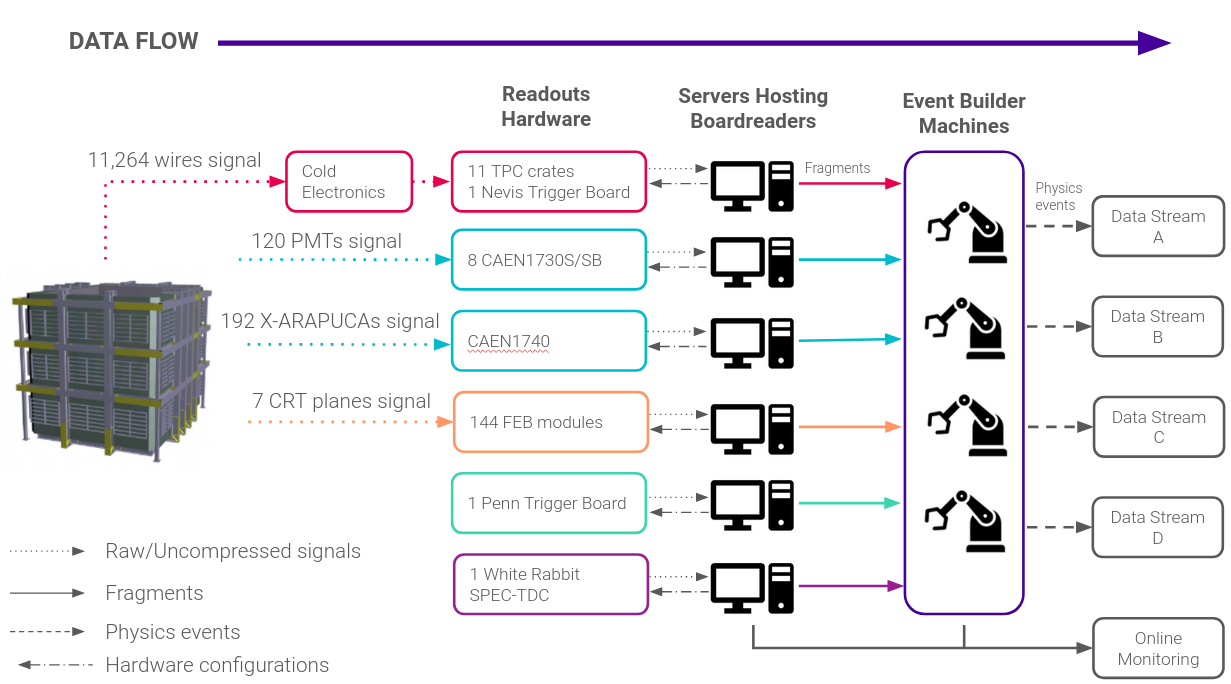
\includegraphics[width=1.0\textwidth]{DAQ_Overview}
\caption[DAQOverview]{
The DAQ system at SBND consists of six subsystems, with four dedicated to detection subsystem readouts for the TPC, CRTs, PMTs and X-ARAPUCAs, while the remaining two facilitate triggering and timing functionalities.
Each hardware component is accompanied by a corresponding software boardreader, serving as a communication bridge between the hardware and the event builder machines.
The event builders assemble a physics events and send it to different data streams for storage.
}
\label{fig:daqOverview}
\end{figure}

The DAQ software framework is provided by the \textit{artdaq Toolkit}, developed by the Real-Time Systems Engineering Department of Fermilab's Scientific Computing Division \cite{artdaq_note}.
The software acts as the backbone of the communication between the hardware components and the event builder machines.
The following section provides an overview of the DAQ workflow at SBND as illustrated in Fig. \ref{fig:daqOverview}, describing how signals are acquired from the detection hardware and subsequently digitized by boardreaders and assembled into a physics event.

%describe boardreader fragment
Within the \textit{artdaq} framework, each discrete hardware readout component has a corresponding software, known as a boardreader, facilitating communication between the readout electronics and the event builder machines.
The boardreader can send configurations directly to the hardware in one direction and retrieves data from the hardware in the opposite direction.
The data is packaged into a digitized format called a fragment as depicted in Fig. \ref{fig:fragmentDiagram}. 
The fragment class includes a header containing experiment-specific information essential for event building, an optional metadata, and a data payload storing the hardware-defined data.
A fragment is generated by the boardreader when its corresponding hardware readout receives a trigger.
The timestamp of the trigger arrival is encoded in the fragment header, which is known as the fragment timestamp.
This timestamp is the crucial value in the event building process.

\begin{figure}[htbp!] 
\centering    
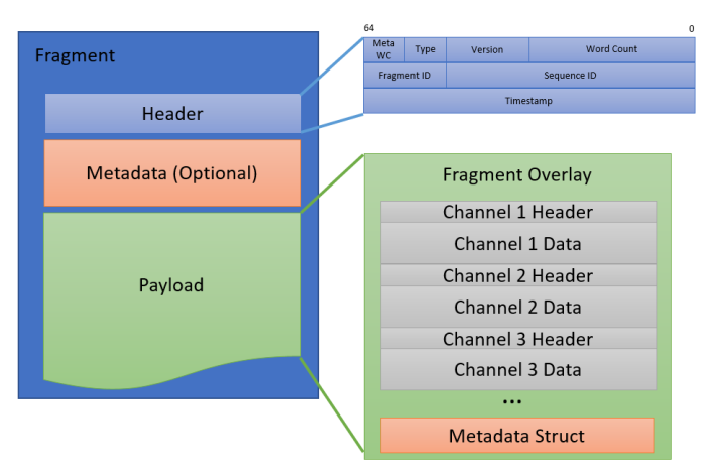
\includegraphics[width=0.6\textwidth]{Fragment_Diagram}
\caption[FragmentDiagram]{This diagram illustrates the fragment class defined by the \textit{artdaq Toolkit}. The header contains information needed for event building, of which the key information is the fragment timestamp. Optionally, the metadata structure contains hardware configurations. The payload is designated for storing data from the hardware readout, of which the data structure is pre-defined by the hardware. }
\label{fig:fragmentDiagram}
\end{figure}

%what is push/pull
Once fragments are generated, boardreaders can send them to the event builders in either one of the two configurations: push or pull. 
When operating in the push configuration, the boardreader actively sends fragments continuously at the rate at which the fragments are generated.
The sequence ID of the fragments determines the sequence ID of the built event, ensuring  that every fragment is built as a single event.
With each fragment sent, the push boardreader also creates a request message, which is multicast to all other boardreaders currently in pull mode.
This request message contains the timestamp of the push fragment. 

In contrast to the push configuration, the boardreader in the pull configuration stores the fragments in its buffer as the fragments are being generated.
These fragments are sent to the event builders only upon receiving a request message.
To determine which fragments to send, the boardreader has a configurable parameter called pull window, which specifies a time window relative to the timestamp of the request message.
The pull boardreader checks its buffer and selects the fragments with timestamps falling within this defined time window.
The selected fragments that meet the timestamp requirement are then dispatched to the event builders.
Subsequently, the event builder machines compile this set of fragments, together with one single fragment from the push boardreader that initially generated the request message, into a single event.
The sequence ID of the resulting event is determined by the push fragment.

\begin{figure}[htbp!] 
\centering    
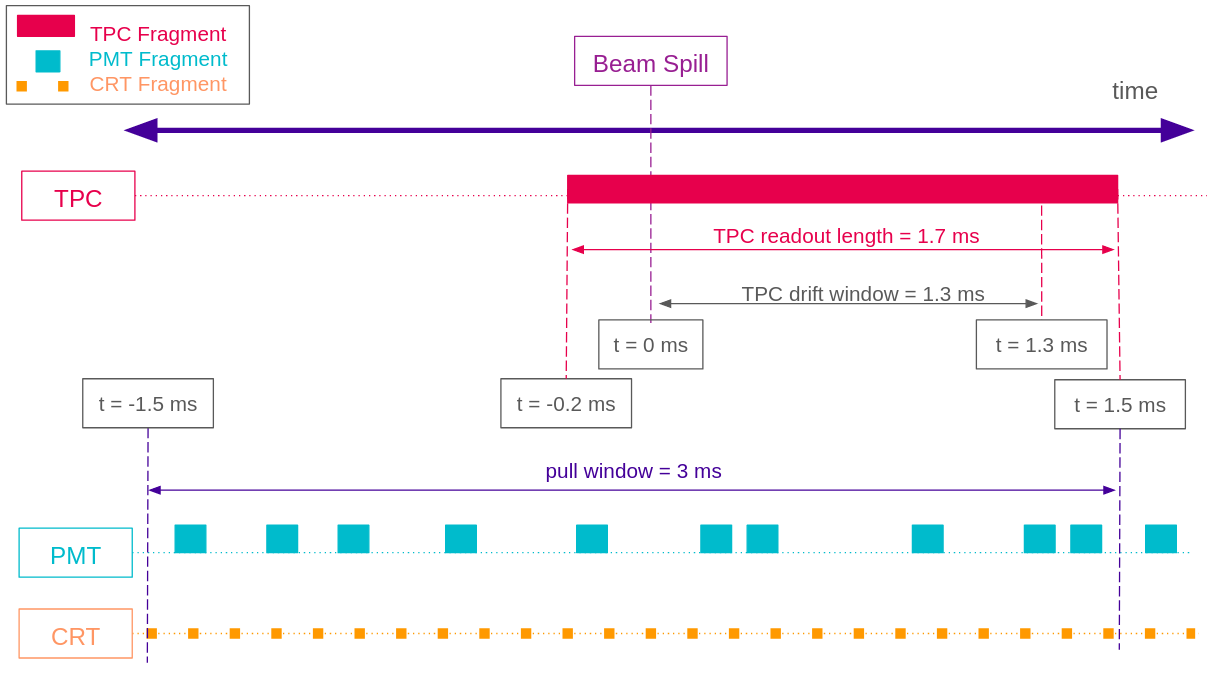
\includegraphics[width=1.0\textwidth]{SBND_Event_Structure}
\caption[SBNDEventStructure]{
This cartoon depicts a physics event structure at SBND, where the time axis is centred at 0 for when the beam spill begins. 
The event contains TPC fragments of readout length 1.7 ms to fully cover the drift window of an ionised electron from cathode to anode. 
The fragments generated by the PMTs and CRTs readouts are included 1.5 ms before and after the beam spill starts. 
The time asymmetry of the event structure is due to scintillation photon signals are produced and digitised much faster compared to electron signals.}
\label{fig:SBNDEventStructure}
\end{figure}

%describe an event structure
A physics event during at beam spill at SBND is built based on the structure shown in Fig. \ref{fig:SBNDEventStructure}, using the fragments from the three detection systems: TPC, PMTs and CRTs.
\footnote{13th November 2023: The DAQ hardware and software for the X-ARAPUCAs is under development and therefore, not be included in this thesis. }
Within this structure, there is only one push boardreader that increments the event sequence ID counter whilst the remaining boardreaders run in pull configuration.
The push boardreader is called the Nevis Trigger Board (NTB), which is a component of the hardware complex to readout the TPC data. 
The PTB sends a single Event trigger to the NTB that coincides with the start of the BNB beam spill if it determines a neutrino event occurs.
This generates a TPC fragment has a readout length of 1.7 ms, that fully covers the TPC drift length of 1.3 ms, and includes a padding of 0.2 ms before and after the drift.
The Event trigger timestamp is encoded in the NTB fragment header.

Meanwhile, the boardreaders for the PMTs and CRTs are in pull mode.
The PTB sends multiple Flash triggers to the PMTs readouts throughout the beam spill and CRTs readouts are self-triggered independently.
The fragment readout lengths from the PMTs and CRTs readouts are much shorter compared to TPC fragments, in the order of $\mu$s and ns respectively.
The pull window is defined to be 3 ms centred on the timestamp of the NTB fragment, to include PMTs and CRTs fragments generated 1.5 ms before and after the beam spill starts.
The event builders then package all the these fragments together to form a physics event.

%event asymmetry
The event structure has an asymmetry in time due to the physics characteristics of photon signals, detected by the CRTs and PMTs, and electron signals, detected by the TPC wires.
Photon signals are much faster than electron signals.
A photon produced in CRT scintillator strip takes approximate 5 ns to travel from the far end of the strip until the readouts.
A photon produced in the TPC takes maximum 15 ns to arrive at the PMTs from the scintillation location.
An ionised electron produced at the same time in the TPC takes 1.3 ms to fully drift from the cathode to the anode.
Therefore, scintillation photon signals produced during the beam spill need be digitized and readout much earlier compared to the electron signals.

%describe a data stream
After the event builder machines complete building a physics event, the resulting event can be filtered and sent to various locations for serving different downstream analysis purposes. 
This process is commonly referred to as data streaming.
The \textit{artdaq Toolkit} provides options to add customisable filtering steps in real-time, such that the event builders can apply complex software metrics based on the fragment contents of an event.
Once an event passes the filter, the event builders send it to a location defined by the filter.
If an event does not pass the filters, it will be dropped in real-time.

\begin{figure}[htbp!] 
\centering    
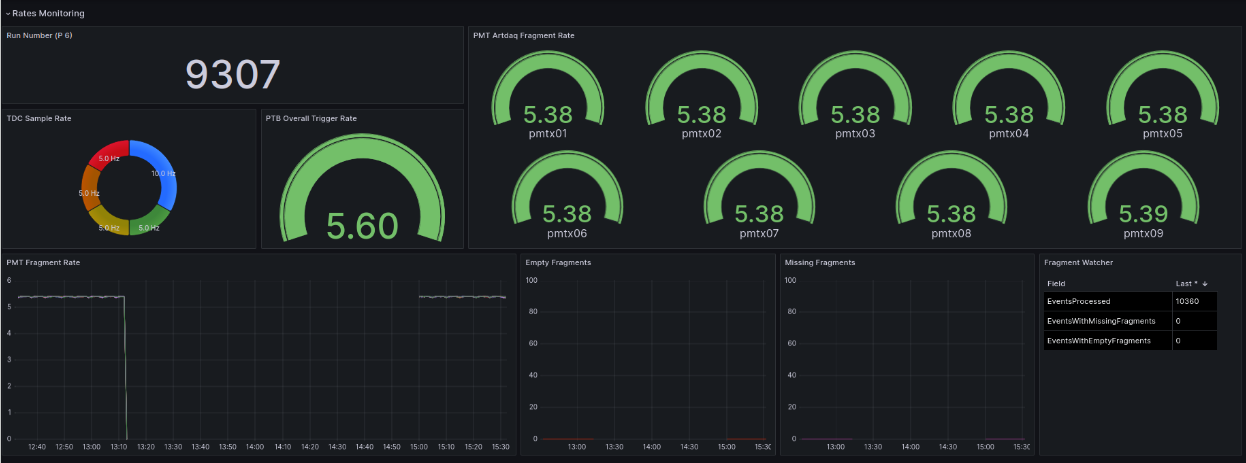
\includegraphics[width=1.0\textwidth]{Grafana}
\caption[Grafana]{
This screenshot displays a section of the Grafana monitoring website for the boardreaders of the PMT DAQ.
Some key information to quickly evaluate the status of the PMT boardreaders are shown.
For example, the fragment generation rate is expected be consistent with the trigger rate sent by the PTB whilst the empty fragment rate and the missing fragment rate stay flat at zero.
}
\label{fig:Grafana}
 \end{figure}

\begin{figure}[htbp!] 
\centering    
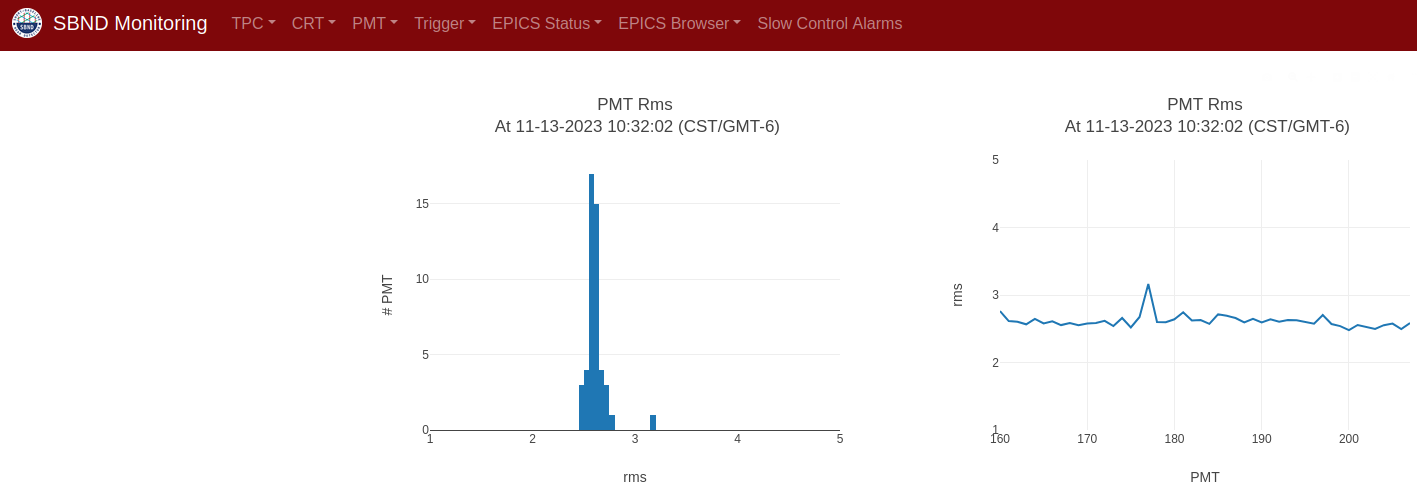
\includegraphics[width=1.0\textwidth]{Minargon}
\caption[Minargon]{
This screenshot displays a section of the Minargon monitoring website to evaluate the quality of data acquired by the PMT DAQ.
For example, a metric shown here is the waveform baseline RMS, plotted as a histogram (left) and plotted with respect to the fragment timestamp (right).
This metric provides monitoring of the baseline equalisation and stability over time.
}
\label{fig:Minargon}
\end{figure}

%data monitoring?
The \textit{artdaq Toolkit} also has a built-in process the bridges the event builder machines and online monitoring platforms.
Whilst running in real-time, fragments from boardreaders and physics events can be sent to the platforms for different monitoring purposes.
SBND currently employs two online platforms that monitors the health of the DAQ: Grafana and Minargon.
Grafana, as displayed in Fig. \ref{fig:Grafana}, provides real-time monitoring of the status of processes being run by boardreaders and event builders. 
Grafana monitoring also extends to include some status of the respective hardware component for each boardreader.
Minargon, as displayed in Fig. \ref{fig:Minargon}, provides real-time the data quality monitoring. 
This online monitoring process applies simple reconstruction and event display in order to quantitatively verify the physics characteristics of an event. 
The author has worked extensively on developing the monitoring processes for the DAQ of the PMTs on both Grafana and Minargon monitoring platforms during her PhD course. 

%********************************** %Second Section  **************************************
\section{Timing Reference System of the Data Acquisition}
\label{sec4TimeRef}

%short description of why need timing reference
The event building process of the DAQ relies entirely on timestamps from the fragment headers to construct a meaningful physics event.
Hence, it is crucial that the timestamp generated by each subsystem readout electronic is generated with a high level of precision and synchronisation.
SBND aims to achieve timing precision of the DAQ hardware and software readout components in the order of nanoseconds to fully leverage the physics capabilities.
The strategy is to utilise the White Rabbit (WR) timing system.

%description of WR timing 
The WR timing system is a collaborative project developed at the European Organisation for Nuclear Research (CERN) and is now a widely-used synchronisation solution in scientific community \cite{WR_paper}.
The WR has the capability to offer fully deterministic time transfer with sub-nanosecond accuracy over distances exceeding 80 kilometers.
The system is currently installed in both the ICARUS and SBND detector buildings.
The installation serves the dual purpose of ensuring timing precision within a single experiment as well as timing synchronisation across the two experiments. 
The application of the WR timing system at SBND for time transferring and timestamping are detailed in section \ref{subsec41TimeRef} and section \ref{subsec42TimeRef} respectively.

\subsection{Time and Frequency Transfer To Subsystems}
\label{subsec41TimeRef}

%Time Transfer Concept
The WR timing system consists of a Grandmaster WR switch that distributes time and frequency to all other WR switches within the WR network via optical fibre links.
The WR switch has dynamic calibration and thus, is a very reliable and robust delivery system.
The system ensures that the Pulse Per Second (PPS) signal, which has the frequency of 1 Hz, from all the slave WR switches in the network are aligned to the Grandmaster's PPS signal with sub-nanosecond accuracy and tens of picoseconds precision. 
Moreover, the Grandmaster WR switch installed at the SBND detector Building is connected to an atomic clock that is locked to a global navigation satellite system. 
As a result, the time and frequency distributed by the WR system are derived from the International Atomic Time (TAI) and the Coordinated Universal Time (UTC).

The Grandmaster switch currently distributes time to two independent WR switches, located at two different servers in the DAQ system.
One of the server houses several SVEC-FD modules, which are Fine Delay (FD) cards carried by Simple VME FMC Carrier (SVEC).
The SVEC-FD module is a high precision pulse generator, with 10 ps resolution and timebase accuracy of 2.5 ppm when used on a WR network.
Each module can output four independent pulses at a time.

\begin{figure}[htbp!] 
\centering    
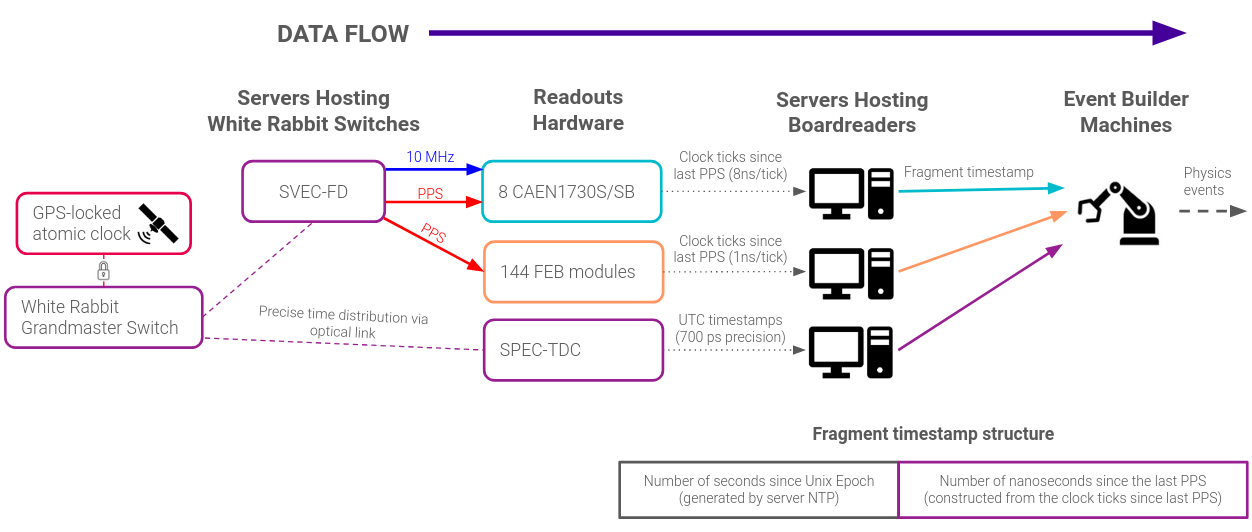
\includegraphics[width=1.0\textwidth]{time_transfer}
\caption[timeTransfer]{
This cartoon displays timing distribution from the WR Grandmaster switch to the electronic readouts for the PMTs and CRTs.
From the Grandmaster switch, the time is transferred to the SVEC-FD modules, which generates highly precise PPS signals and 10 MHz clock.
The 10 MHz clock is locked to the PPS signals such that the clock is issued on the rising edge of the PPS signal.
These frequencies are input to the electronic readouts to that produce clock ticks since the last PPS arrived.
The fragment timestamp is then generated by the boardreader using the clock ticks information, which is used by the event builders to assemble fragments into a physics event.
}
\label{fig:timeTransfer}
\end{figure}

%description of timing provided to each subsystem: PPS/ 10 MHz Clock?
The modules are used to generate clock frequencies to subsystem hardware components, which behave as the master clock that the internal clocks of the subsystem hardware can latch onto.
Since the modules are part of the WR network, the clock frequencies are synchronised with each other, and thus, so are the subsystem internal clock.
The standard clock frequency is the PPS signal and 10 MHz. 
Depends on the specification, each subsystem hardware readouts must have an input for the PPS signal, an optionally an input for the 10 MHz clock.

As illustrated in Fig. \ref{fig:timeTransfer}, this set up ensures that clock ticks generated by each electronic board is reference with respect to the last PPS arrived, and thus sharing the same time frame of reference to the PPS.
As the boardreader packages the data into fragment format, it creates the timestamp in the fragment header.
The timestamp is in UTC format and its structure consists of two parts, the second part and the nanosecond part.
The second part is the total of number of seconds since the Unix Epoch on 1st of January 1970 at UTC, which is generated by the server hosting the boardreader under the Network Time Protocol (NTP).
The nanosecond part is the number of nanosecond since the last PPS arrived, derived from the clock ticks since the PPS generated by the readout electronics.
This timestamp is subsequently used by the event builders to put the fragments together into an event.
Thus, the DAQ workflow places a vital importance on the internal clocks of each hardware readout, which are further explored in section \ref{sec4InternalClock} and section \ref{sec4PMT} for the CRTs and PMTs electronics respectively.

\subsection{Precise Timestamping}
\label{subsec42TimeRef}

%Precision Timestamp concept
%description of SPEC TDC
The Grandmaster switch is also connected to server node that hosts the SPEC-TDC module, which is short for a FMC Time to Digital Converter (TDC) carried by a Simple PCIe FMC Carrier (SPEC).
The SPEC-TDC can timestamp five input signals independently with a precision of 700 ps.
The output timestamps are in UTC standard such that it contains the last whole second in UTC format and the number of nanoseconds since the last whole second.
Thus, the timestamps are in the same time frame of reference with respect to the PPS signal.
Moreover, the SPEC-TDC also has its own boardreader so that the recorded timestamps can be built within an event, and available for downstream analysis.

% SPEC TDC 
Following Fig. \ref{fig:SPECTDC}, one application of the SPEC-TDC is to synchronise the DAQ system with respect to the beam.
This can be done by employing the SPEC-TDC to timestamp two important beam signals, that can provide status of the BNB beam.
The first one is the Booster Extraction Signal (BES), which is an early warning signalling when protons are extracted in the Booster cycles.
The second one is the Resistor Wall Monitor (RWM), which measures the instantaneous beam current onto the BNB target.
The RWM signal arrives at the SBND detector building almost simultaneously with the beam itself, and thus is used to signify when the beam arrives.
The delay between the BES and the RWM signal is approximately 333 us.
Recording the timestamps of these beam signals provides valuable tools for various monitoring purposes. 

\begin{figure}[htbp!] 
\centering    
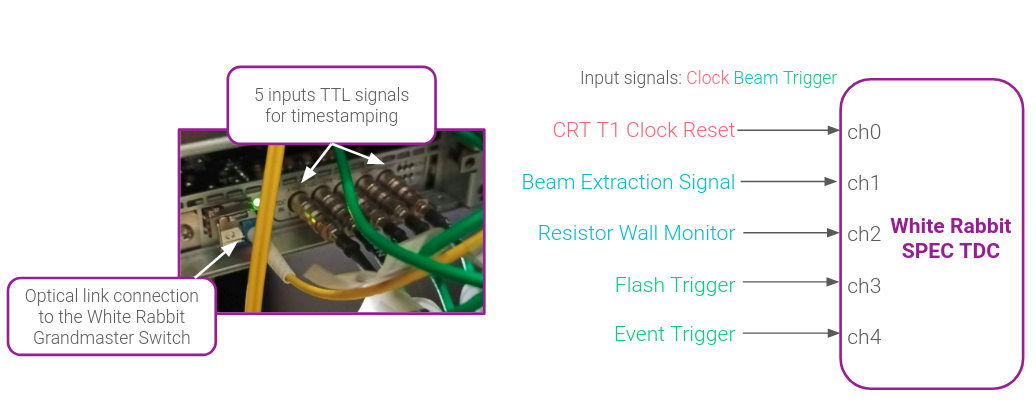
\includegraphics[width=1.0\textwidth]{SPEC_TDC}
\caption[SPECTDC]{
The photograph on the left shows the SPEC-TDC module installed at the sbnd-clk01 server.
The diagram on the right shows the input signals into the module for timestamping purposes.
}
\label{fig:SPECTDC}
\end{figure}

Additionally, the SPEC-TDC timestamps the trigger signals, which offer insights of the DAQ synchronisation with respect to the triggers. 
Referencing back to Fig. \ref{fig:daqOverview}, an event contains two types of trigger: a single Event trigger and multiple Flash triggers. 
Both types of triggers are issued relative to the beam, such that the PTB only issues triggers within the beam spill window.   
The recorded trigger timestamps can be cross referenced to the beam timestamps, and thus, enabling monitoring of the triggering synchronisation to the beam in real-time.

The last available channel of the SPEC-TDC used to record the clock reset signals for the CRT readouts. 
Upon receiving this signal, the CRT readouts reset the counters of its internal clocks.
Thus, monitoring this signal provides direct measurement of the resolution of the CRT readouts clocks.
This study was carried out by the author and is described in section \ref{sec4InternalClock}.

SPEC-TDC capabilities of high precision timestamping can be leveraged for physics application.
Recording both the timestamps of the beam and trigger signal in a single event opens up venues for various physics applications. 
One example is the characterisation of timing resolution the DAQ hardware readouts, by directly comparing the timestamps produced by the hardware against the timestamps of the SPEC-TDC given that both share the common time reference to the PPS signal.
Furthermore, it provides useful timing information for downstream analysis, for example, applying timing correction for hardware resolution and providing alternative method for event timing reconstruction. 
The SPEC-TDC applications are to be explored in the future includes nanosecond timing reconstruction, allowing for physics application such as cosmics rejection and physics searches between neutrino bucket.

The author has worked extensively on installing, testing and calibrating the SPEC-TDC over her visits at Fermilab.
The  conducted work included the hardware installations of the SPEC-TDC, by testing out two different PCIe connections on two different servers. 
One server can hold the SPEC-TDC horizontally whilst the other can hold the SPEC-TDC vertically. 
The latter was chosen due to better structural support and ventilation to host the SPEC-TDC.
The software boardreader of the SPEC-TDC also had some improvements implemented by the author, namely, better timestamp correction and higher data processing rate.
The calibration work included measuring a constant offset introduced by the SPEC-TDC hardware to be 58 ns.

%********************************** %Second Section  **************************************
\section{Timing Precision of the Cosmic Ray Tagger DAQ}
\label{sec4InternalClock}

The timing resolution of the CRT readout electronics is evaluated in the following section.
%CRT FEB
The CRT detection system consists of 7 CRT planes, and is readout by 144 Front End Board (FEB) modules \cite{crt_note}. 
A single FEB module a multifunctional board and is capable to serve 32 channels, one channel per Silicon PhotoMultiplier (SiPM). 
First it can provide a bias voltage which can be adjustable for individual SiPM as well as signal amplification and shaping.
Once the signal is shaped, the FEB can apply signal discrimination and self-triggering, such as coincidence for each pair of SiPM and coincidence across multiple FEBs.
Once the signal passes the trigger, it is digitised and timestamped with respect to the reference clock.
The data is stored in a buffer and readout via Ethernet connection.
The following section focuses on the characterisation on the timing resolution of the FEB module.

%Do I need to explain what CRT panel is made of? Or should I explain it in the detector chapter?

\subsection{Front End Board Clock}

The clock of a FEB module is a TDC unit that consists of a coarse counter of 4 ns per tick (250 MHz frequency). 
A high resolution time interpolation method is implemented within the TDC clock cycle to improve the counter to 1 ns per tick \cite{crt_clock}.
The clock resets its counter upon receiving an input reference pulse.  
The generated timestamp is the number of ticks since the clock last resets.
The FEB can also timestamp the arrival of the reference pulse and save it as special non-physics events, called clock reset event.
The timestamp of a clock reset event is essentially the counter of the clock before getting reset.

The FEB module has two internal clock counters, of which each can be reset independently via external TTL signal into LEMO connections of the module.
The first internal clock is known as the T0 clock, which is reset by the PPS signal issued by the SVEC-FD cards. 
This clock produces T0 timestamp, referencing to the PPS frame of reference.
The second internal clock is known as the T1 clock, which is reset by the BES signal\footnote{21st November 2023: At the time of writing, there is consideration to use the BES signal issued by the PTB hardware. The plan is not yet finalised}.
This signal has a higher frequency compared to the PPS signal, averaged at 5.5 Hz.
The generated T1 timestamp is expected to have a higher precision since the T1 clock is reset more frequently. 
Because of this clock system, the FEB module generates two independent timestamps, T0 and T1 with respect to the PPS and BES signal, for every recorded event.
The FEB module also records two types of clock reset event for the T0 and T1 clock.

\subsection{Evaluation of Timing Resolution}

%CRT Sharp Set Up
Over the summer of 2022, the author has travelled to Fermilab to conduct the work on evaluating the timing resolution of the FEB module.
It was conducted using a temporary set up for commissioning usage, called CRT Sharps as photographed in \ref{fig:crtSharps}.
The CRT Sharps was made of two sets of four CRT panels. 
Each set of panels was placed upstream and downstream of the SBND detector cryostat, centred on the BNB location.
The panels were readout by a total of 8 FEB modules, 4 upstream and 4 downstream.
The CRT Sharps was commissioned during the period at which the BNB beam was on. 
The triggering condition was to have signal coincidences between the upstream and downstream panels during the beam spill.
This was to ensure that CRT Sharps setup only recorded events produced by muons coming from beam neutrinos and therefore, functioned as a beam telescope.
The analysis described below used dataset recorded by the CRT Sharps during the summer and fall of 2022.

\begin{figure}[htbp!] 
\centering    
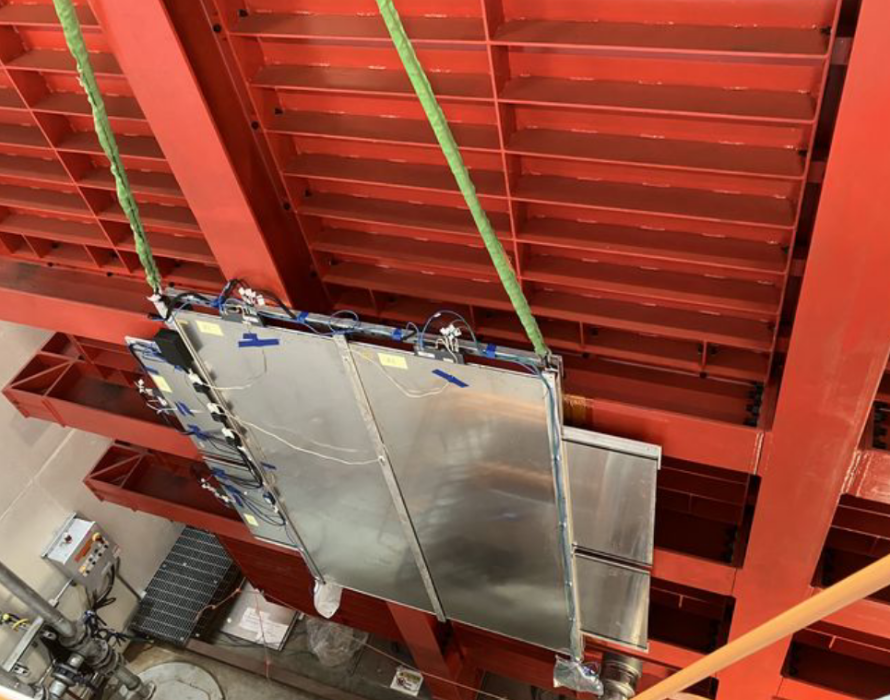
\includegraphics[width=0.6\textwidth]{crt_sharps}
\caption[crtSharps]{
The photograph shows the downstream panels of the CRT Sharps set up, hanging on the back wall of the SBND cryostat. 
The CRT Sharps was positioned precisely such that it was centred on the BNB beam.
}
\label{fig:crtSharps}
\end{figure}

%T0 Clock
%As previously described, the FEB can store the timestamps of clock reset events, which are the timestamps at which the input reference signals arrive at the FEB module.
For the T0 clock characterisation, the T0 clock reset events were of interest.
The timestamp T0 of the T0 clock reset event is the number of nanosecond since the FEB module last receives a PPS signal to reset its T0 clock.
To measure the clock variation, one can simply compare this timestamp with respect to a whole second.
An example is shown in Fig. \ref{fig:UpstreamT0StabilityCombinedBoard79} for a single FEB module numbered 79.
The T0 timestamp of the T0 clock reset event shows variation within roughly 2 ns of every second. 
The standard deviation of this timestamp distribution is the direct measurement of the T0 clock variation.
This indicates that the FEB module 79 consistently received the PPS signal to reset its T0 clock and the resolution of the T0 clock of the FEB is of the order $\mathcal{O}$(2 ns).
This measurement was repeated for other FEB modules of the CRT Sharps and the finding was consistent.

\begin{figure}[htbp!] 
\centering    
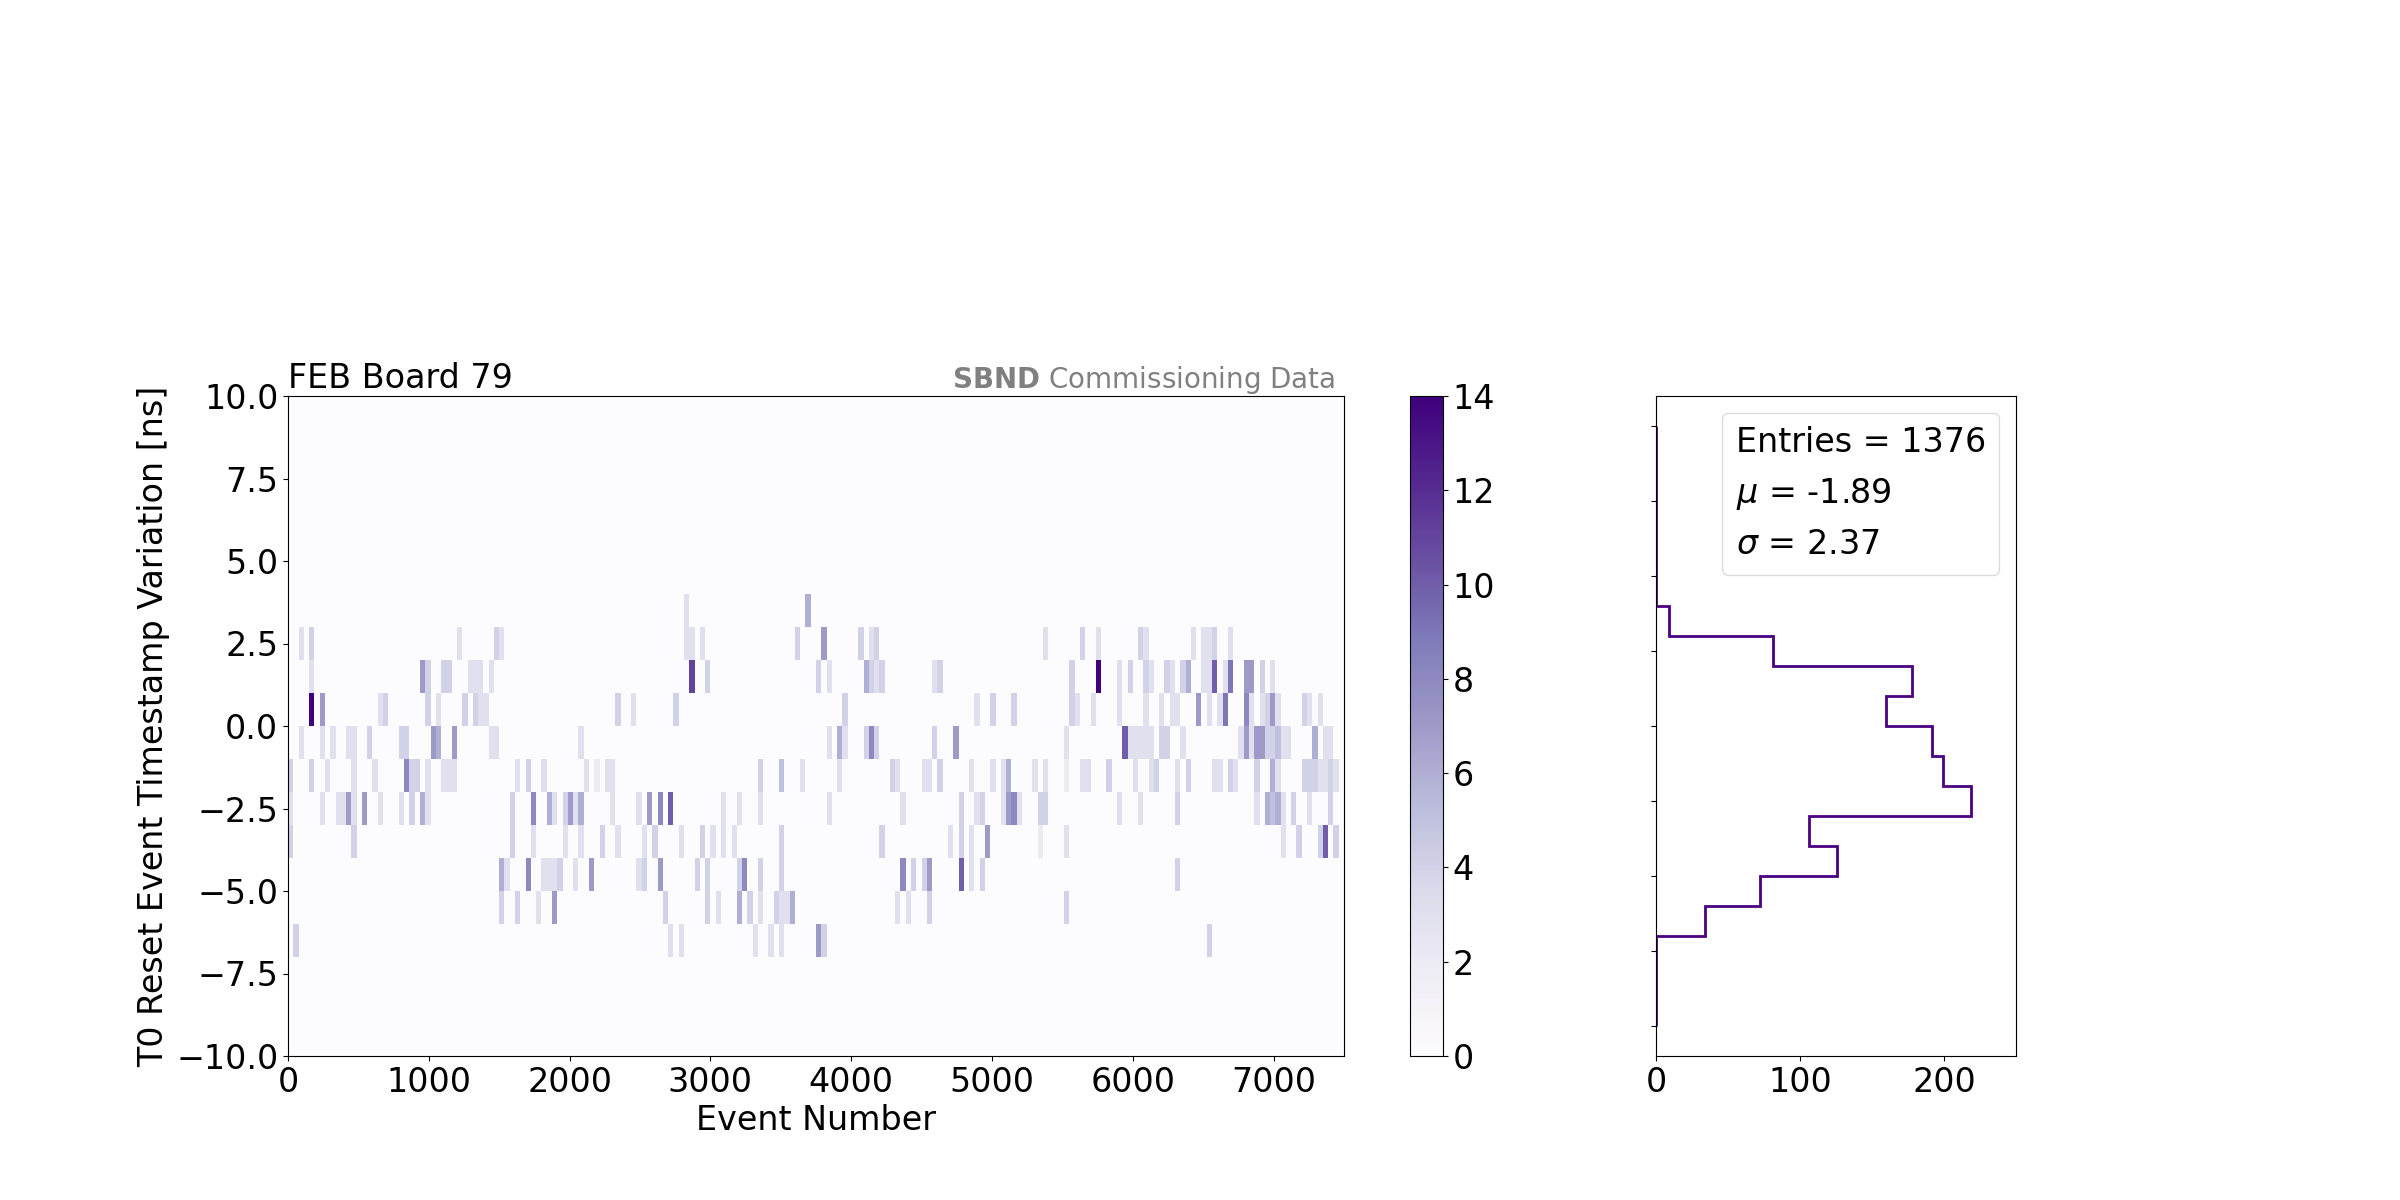
\includegraphics[width=1.0\textwidth]{upstream_T0stability_combined_board79}
\caption[UpstreamT0StabilityCombinedBoard79]{
The plots display the T0 timestamp of the T0 clock reset events with respect to a whole second. 
The timestamp variation indicates the resolution of the T0 clock, which is of the order $\mathcal{O}$(2 ns).
The left plot shows the timestamp variation with respect to the event number to check for the stability of the clock over a period time whilst the right plot is a histogram to easily check for the spread of the distribution.
}
\label{fig:UpstreamT0StabilityCombinedBoard79}
%\end{figure}

%\begin{figure}[htbp!] 
\centering    
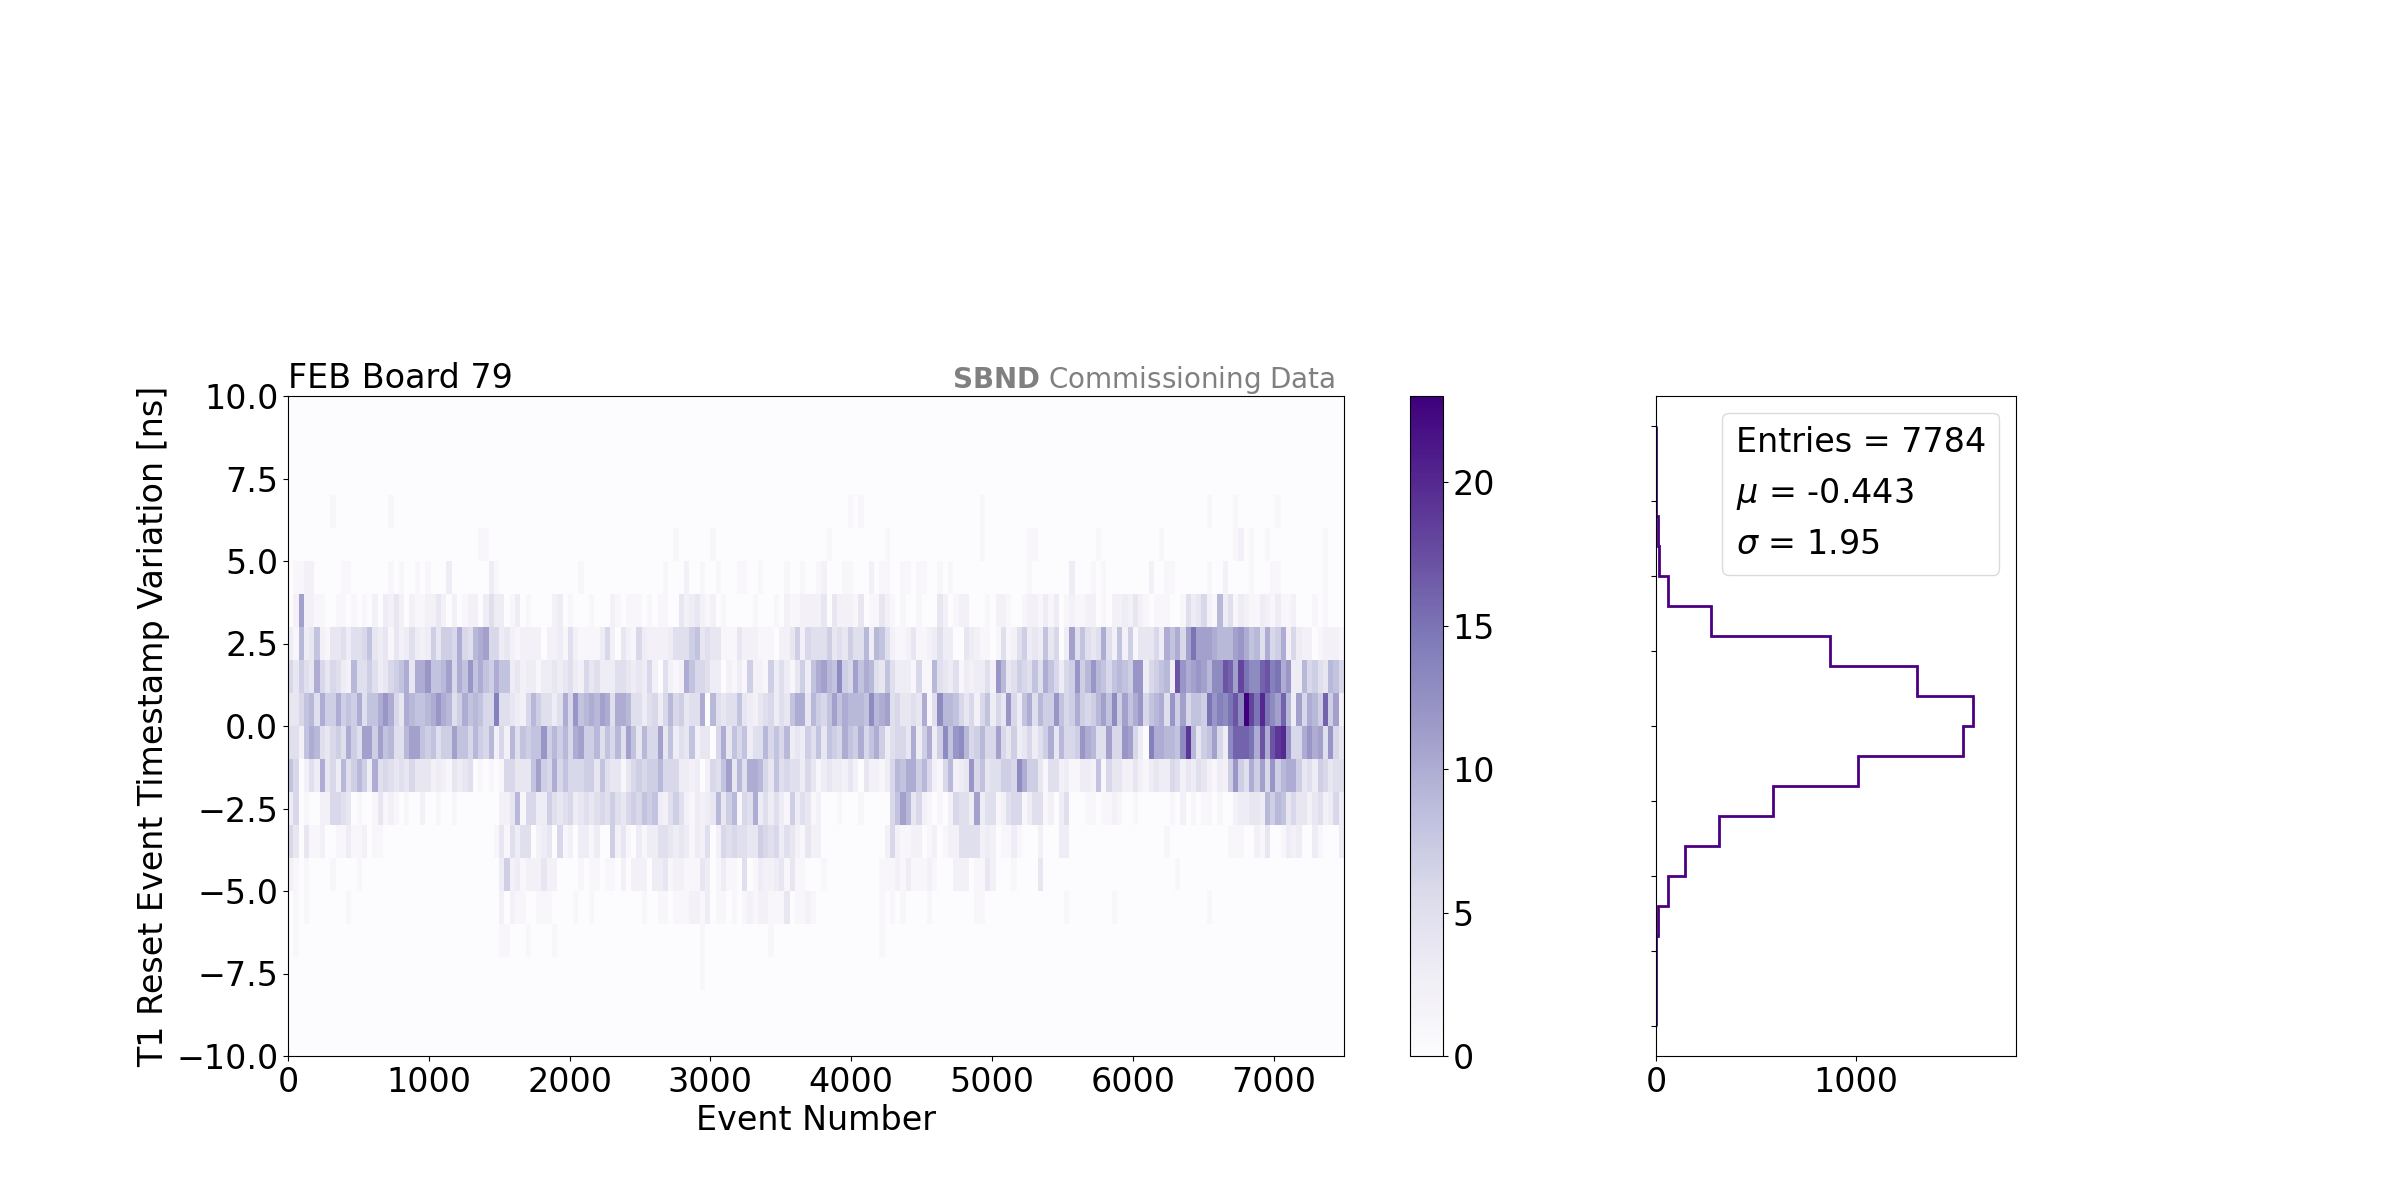
\includegraphics[width=1.0\textwidth]{upstream_T1stability_combined_board79}
\caption[UpstreamT1StabilityCombinedBoard79]{
The plots display the T0 timestamp of the T1 clock reset events, with respect to the SPEC-TDC recorded timestamp of the BES signal. 
The left plot shows that the T1 clock reset event with respect to the event number, indicating that the T1 clock was reset regularly and therefore, stable.
The right plot is a histogram of the time variation distribution, showing a standard deviation of the order $\mathcal{O}$(2 ns).
This resolution is in fact by the resolution of T0 clock given that T0 timestamps are being plotted. 
}
\label{fig:UpstreamT1StabilityCombinedBoard79}
\end{figure}

%T1 Clock 
%As shown previously, the T1 clock of the FEB module is reset by the BES signal.
Similarly for the T1 clock characterisation, the T1 clock reset events were selected and their timestamps were examined, specifically the T0 timestamps.
The timestamp variation was measured by comparing directly against the SPEC-TDC recorded timestamp of the BES signal, given that the SPEC-TDC has a higher precision than FEB internal clocks.
The cable length differences were corrected for the comparison.
%Since the SPEC-TDC is much more precise compared to the clocks of the FEB modules, comparing the T0 timestamps against the SPEC-TDC provides some insights about the clock characteristics.
The comparison is plotted in Fig. \ref{fig:UpstreamT1StabilityCombinedBoard79}, shown for a single FEB module 79.
The plot indicates that the T1 reset events arrived consistently at the FEB module and thus, its T1 clock was reset regularly.
The standard deviation of the distribution does not give direct measurement of the resolution of the T1 clock since the T0 timestamps are being examined. 
In fact, the standard deviation is smeared out by the resolution of the T0 clock, and thus, also of the order $\mathcal{O}$(2 ns).
Even though the intrinsic resolution of the T1 clock can not be directly measured, it is expected to be lower due to more frequent resets.
This measurement was also repeated for other FEB modules of the CRT Sharps and the resulting plots showed similar findings.

Moreover, the T1 clock reset events also provide an additional method to further characterise the T0 clock of the FEB module. 
This can be done by plotting the T0 timestamps variation against the T0 timestamps, as shown in Fig. \ref{fig:Board79T1Drift2d} for the FEB module numbered 79.
The plot indicates the T0 clock can drift overtime.
The T0 timestamp shows a little variation when the T0 clock counter is low, meaning that the timestamp was generated when the T0 clock recently received a PPS signal to reset.
Meanwhile, the T0 timestamp shows a larger variation when the T0 clock counter is high, meaning the timestamp was produced when T0 clock counter was close to a full second.
This illustrates that the precision of the timestamp is influenced by at which part of the cycle the clock counter is currently is in.
It is also possible that the counter can overflow and the resulting timestamps are meaningless.
When this happens, the FEB modules can flag these events and their timestamps need to be invalidated.
The clock drift behaviour is expected to be more prevalent with the T0 clocks than the T1 clocks due to lower reset frequency.

\begin{figure}[htbp!] 
\centering    
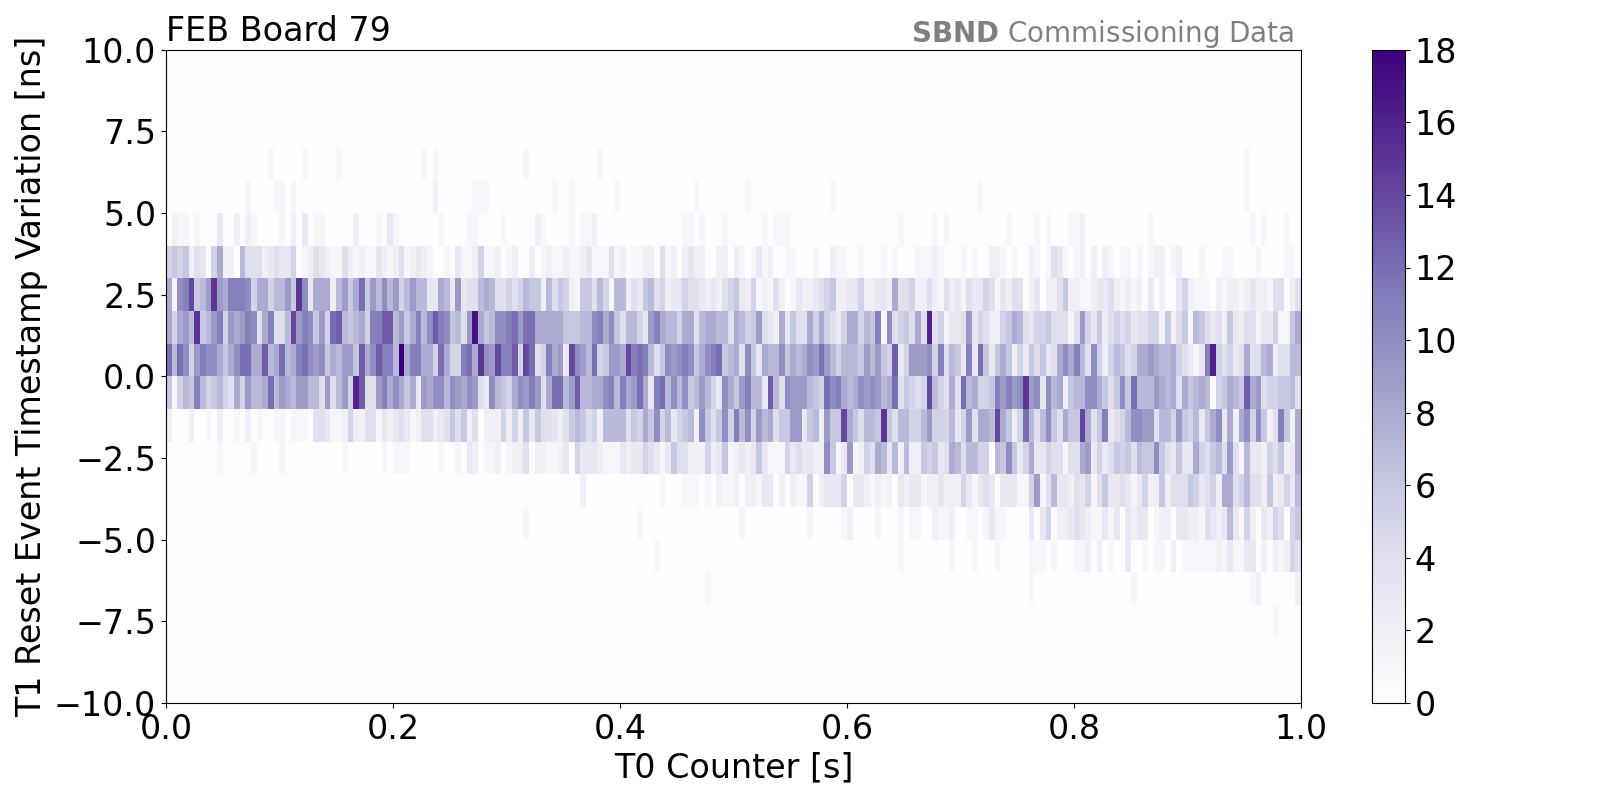
\includegraphics[width=0.70\textwidth]{board79_T1drift_2d}
\caption[Board79T1Drift2d]{
The variation of the T0 timestamp of the T1 clock reset events with respect to the SPEC-TDC recorded timestamp of the BES signal is plotted against the T0 timestamp itself.
This plot demonstrates that the T0 clock can drift such the timestamps shows a little variation at low T0 clock counter and a larger variation at high T0 clock counter.
The clock drift behaviour will be monitored in real-time during physics run to ensure clock stability.
}
\label{fig:Board79T1Drift2d}
\end{figure}

These plots are useful diagnostic tools to characterise the timing of the FEB modules: to examine whether the T0 and T1 clock resolution are stable and of the order $\mathcal{O}$(2 ns), and if the T0 clock drift can be monitored.
It is important to note that the T0 and T1 clocks of the FEB can potentially vary from run to run, and very sensitive to external noises. 
The plots have been reproduced by the CRT working group of SBND during the CRT installation periods and they will also be produced for online monitoring purposes in order to track the clock stability and resolution of the FEB modules.

\subsection{Alternative Timing Reconstruction}

%Having the SPEC-TDC also opens up opportunities for alternative timing reconstruction method. 
The following section explores how the timing information recorded by the SPEC-TDC can be used together with T0 timestamps of the FEB modules for an alternative timing reconstruction method.
The data set recorded by the CRT Sharps contained about 9000 beam events. 
The CRT 2D hit time was reconstructed from coincidental hits of 2 cross scintillator strips, and corrected for cable and propagation delay.
The CRT Hit Time T0 was reconstructed using the T0 timestamp whilst the CRT Hit T1 was reconstructed using the T1 timestamp. 
Typically, timing reconstruction from CRT data only uses the CRT Hit Time T1, whilst this following explores how the CRT Hit Time T0 can also be employed.

\begin{figure}[htbp!]
\begin{subfigure}[h]{0.49\linewidth}
\centering    
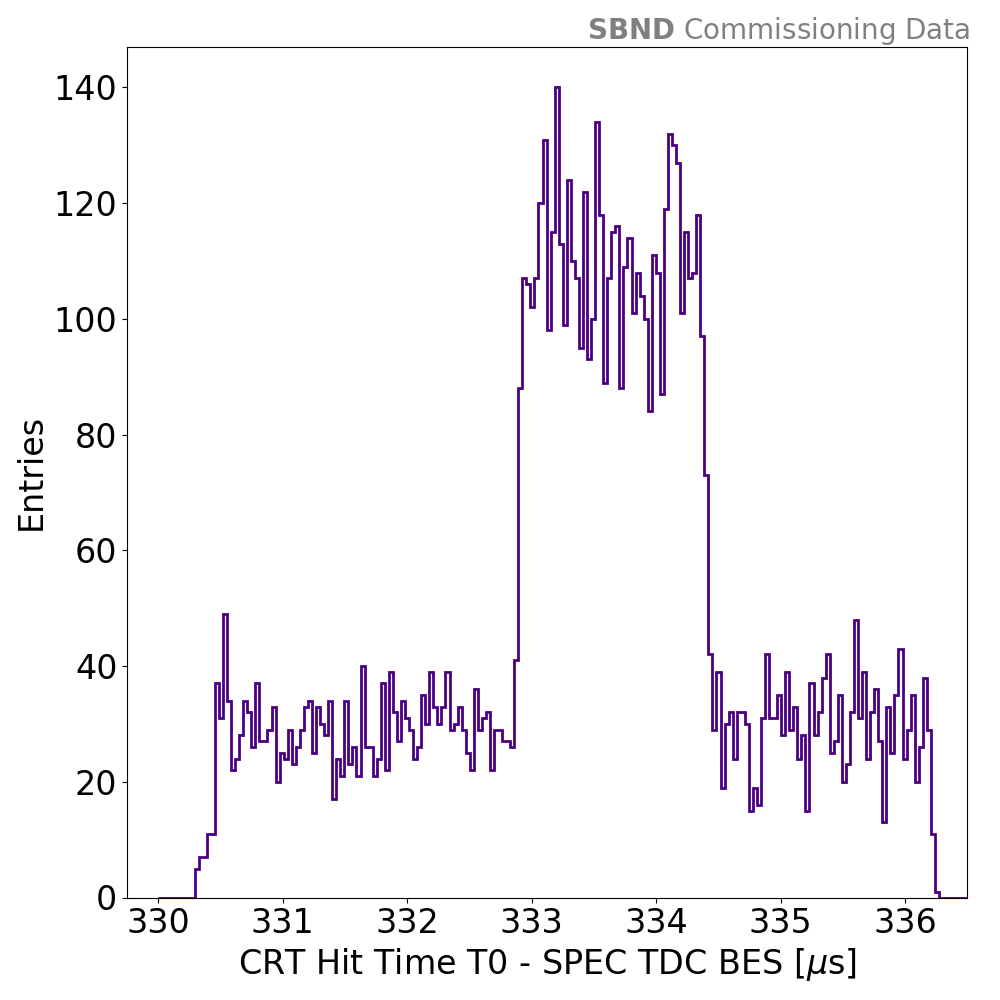
\includegraphics[width=\linewidth]{CRTT0_SPEC_TopHat}
\caption{Reconstructed using CRT Hit T0 Timestamp and SPEC-TDC Timestamp of the BES signals}
\end{subfigure}
\hfill
\begin{subfigure}[h]{0.49\linewidth}
\centering    
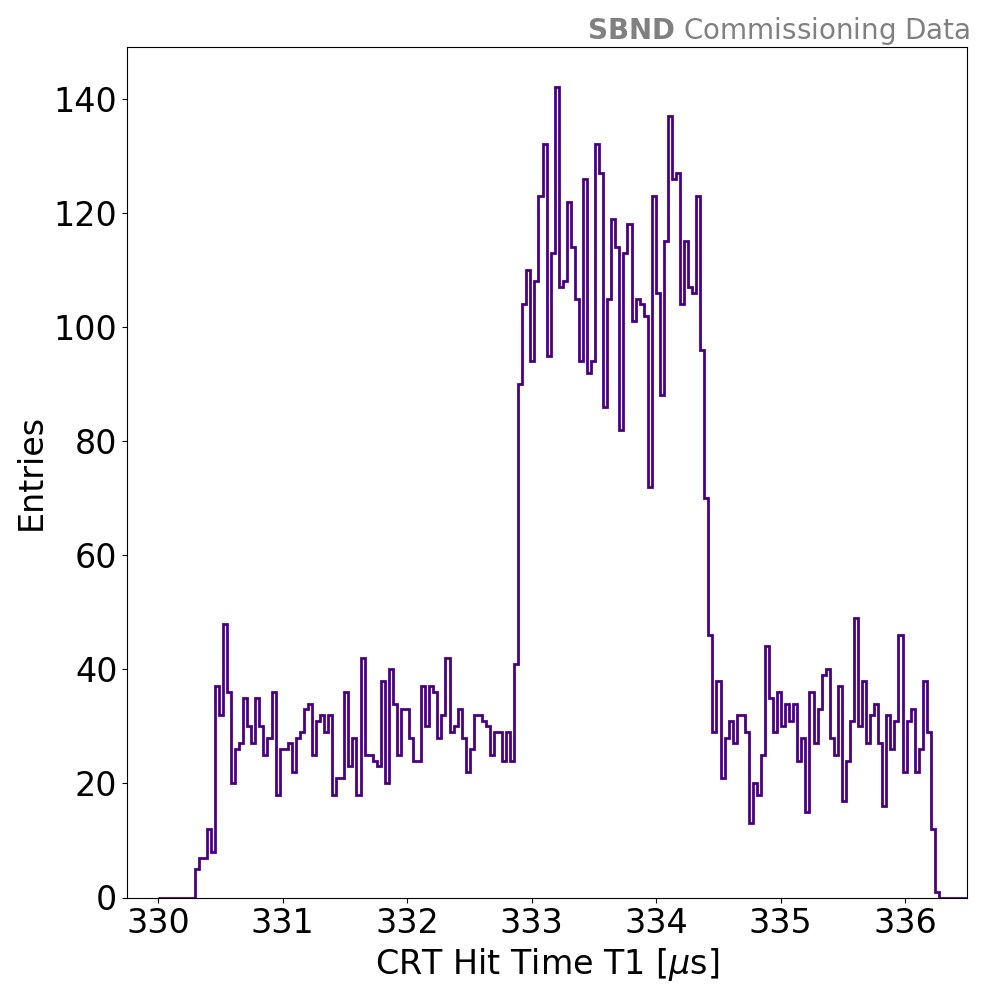
\includegraphics[width=\linewidth]{CRT_T1_TopHat}
\caption{Reconstructed using CRT Hit T1 Timestamp only}
\end{subfigure}%
\caption[topHat]{The reconstruction of the beam spill structure using CRT Hit Time T1 (left) and CRT Hit Time T0 combined with SPEC-TDC timing information (right). 
Both methods are able to reconstruct the "top hat" shape of the beam spill and show good agreement with each other.
}
\label{fig:topHat}
\end{figure}

The first timing reconstruction object is the beam spill as shown in Fig. \ref{fig:topHat} using CRT Hit Time T0 and CRT Hit Time T1 respectively.
Since the CRT Hit Time T1 is essentially the clock counter since the BES signal, the beam spill structure can be plotted directly.
The CRT Hit Time T1 plot shows that the BNB beam spill arrived 333 $\mu$s after the BES signal and lasted about 1.6 $\mu$s.
There is a clear peak at 333 $\mu$s on top of the flat distributions coming from cosmics muons, which indicates the events are indeed produced by the neutrino beam.
In the case of the CRT Hit Time T0, the frame of reference is with respect to the PPS signal, and thus, needs to be shifted relative to the beam time to reconstruct the beam spill structure.
This can be done by subtracting the BES signal timestamped the SPEC-TDC, corrected for cable lengths.
As a result, the beam spill structure can be plotted using both the CRT Hit Time T0 and the SPEC-TDC timestamps, showing a similar result.
The two reconstruction methods show good agreement with each other.
It is important to note that the beam spill structure only requires timing resolution of the order $\mathcal{O}$($\mu$s) and thus, both the CRT Hit Time T0 and T1 surpass this requirement.

\begin{figure}[htbp!]
\begin{subfigure}[h]{0.49\linewidth}
\centering    
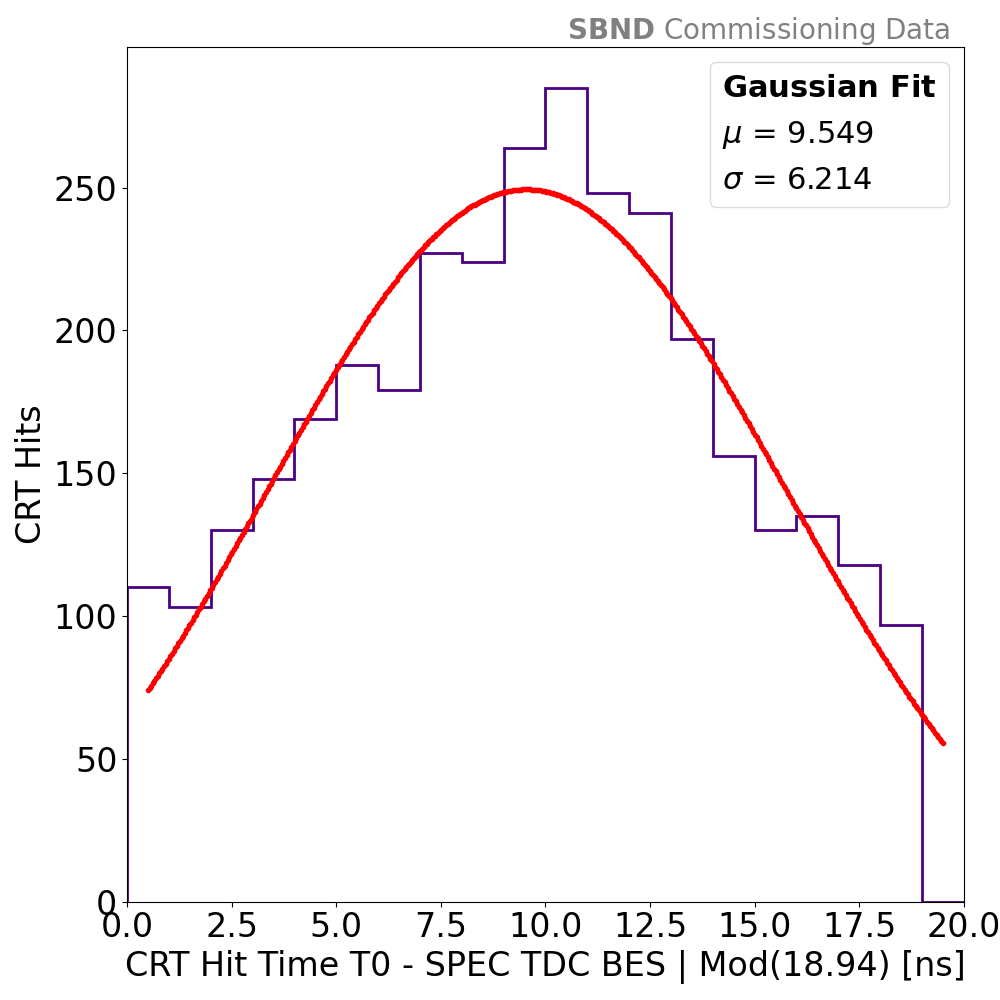
\includegraphics[width=\linewidth]{CRTT0_SPEC_Bucket}
\caption{Reconstructed using CRT Hit T0 Timestamp and SPEC-TDC Timestamp of the BES signals}
\end{subfigure}
\hfill
\begin{subfigure}[h]{0.49\linewidth}
\centering    
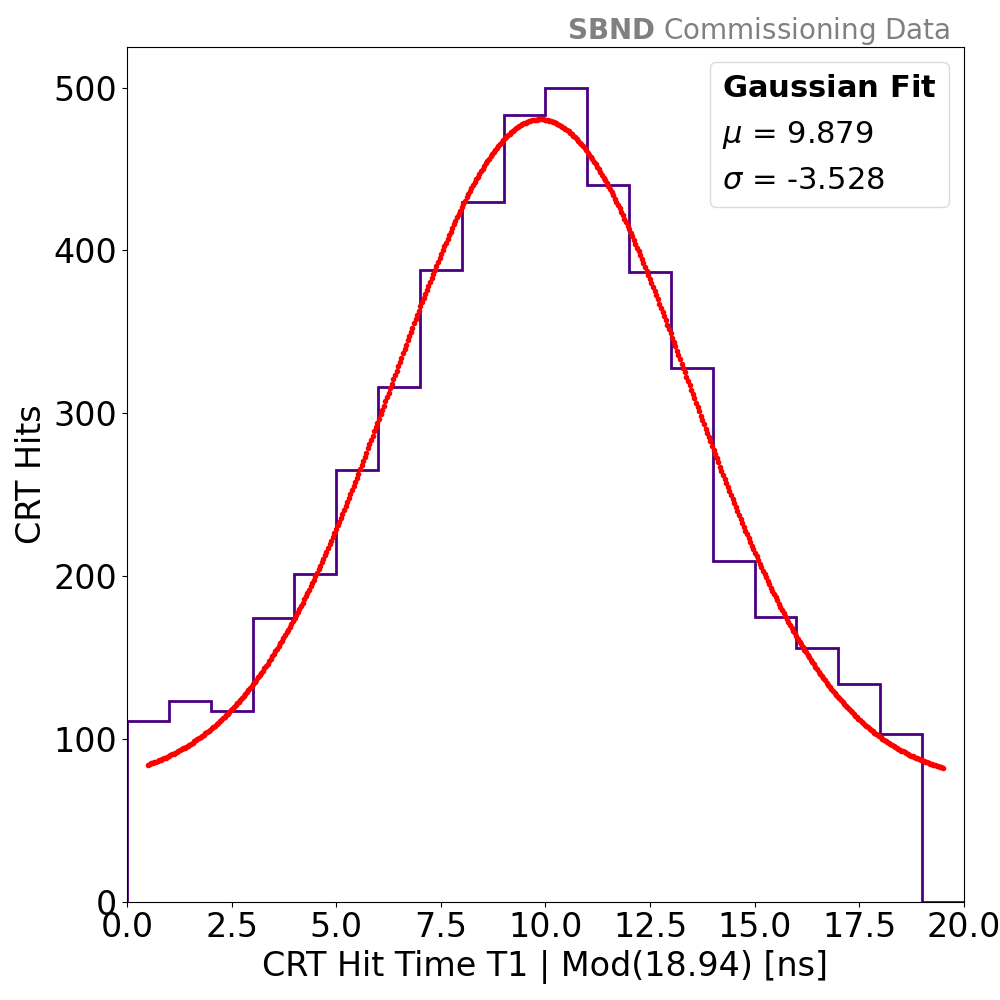
\includegraphics[width=\linewidth]{CRT_T1_Bucket}
\caption{Reconstructed using CRT Hit T1 Timestamp only}
\end{subfigure}%
\caption[beamBucket]{
}
\label{fig:beamBucket}
\end{figure}

The next step was to push the timing reconstruction further by reconstructing the substructure of the BNB beam, to determine if it is possible to resolve the beam buckets.
The BNB beam spill is made of 81 Gaussian neutrino buckets of width 1.3 ns and period of 19 ns.
Given the limited statistics of the sample to fully plot 81 buckets, the buckets were overlay on top of each other by taking the modulo of 18.94 ns of the CRT Hit Time distribution.
The period value of 18.94 ns was measured from data taken between 2017 - 2018, using CRT panels set up inside the empty SBND pit.

The resulting beam bucket plots using CRT Hit Time T1 and CRT Hit Time T0 combined with the SPEC-TDC timestamp of the BES signal are shown in Fig. \ref{fig:beamBucket}.
The CRT Hit Time T1 distribution is able to resolve the beam bucket structure precisely even with a limited statistics.
The CRT Hit Time T0 distribution can also resolve the bucket structure however with less precision. 
The Gaussian shape is more smeared out due to the intrinsic resolution of the T0 clock of the order $\mathcal{O}$(2 ns), which is larger than the width of beam bucket structure.

Whilst this alternative timing reconstruction has potential for more improvements, it shows promising outcomes at an early stage.
Specifically, this demonstrates that the CRT Hit Time T0 can be utilised for timing reconstruction purposes. 
Additionally, combining timestamps recorded by the SPEC-TDC with other hardware subsystems is a versatile tools for multiple purposes, from timing resolution characterisation to timing reconstruction.

%********************************** %Third Section  **************************************
\section{Timing Precision of the Photomultiplier Tube DAQ}
\label{sec4PMT}

%CAEN digitizer
SBND has 120 PMTs as part the Photon Detection System and they are readout by 8 CAENV1730 digitizers \cite{caen_manuals}.
The CAENV1730 digitizer is capable of recording waveforms for 16 channels independently with a sampling rate of 500 MHz.
SBND currently uses the model V1730SB which has a deeper buffer to save longer waveform as well as to handle higher data rate.
The model also offers better waveform baseline stability against temperature fluctuation.
Multiple CAEN digitizers can be synchronised to make up one complex system, such that they all behave as a single digitizer.
Thus, the following section evaluates the timing precision of CAEN digitizer by characterising the synchronisation across multiple digitizers.

\subsection{CAEN Digitizer Clock}
\label{subsec41PMT}
%clock of a single digitizer
The clock distribution of the CAEN digitizer is made up of two clock domains in the hardware: OSC-CLK and REF-CLK.
The OSC-CLK is a fixed internal oscillator that has a frequency of 50 MHz. 
This clock is responsible for handling communication between the motherboard and the mezzanines such as local bus, universal serial bus and optical link.
The REF-CLK handles sampling and triggering frequency via a clock chain.
The source of the REF-CLK can either be internal or external.
For internal mode, the REF-CLK is referenced to the OSC-CLK of frequency 50 MHz.
For external mode, the REF-CLK is fed by an external frequency via the CLK-IN connector. 

%What are the clocks
The REF-CLK is the clock of interest to ensure synchronous sampling and triggering rate, and thus the timing precision of the CAEN digitizers.
The REF-CLK frequency serves as an input to a phase-locked-loop and clock distribution device AD9510, generating three types of frequencies: the ADC sampling clock, the trigger logic clock and the output clock via the CLK-OUT connector.
The ADC sampling frequency, set as 500 MHz, handles the sampling rate of waveforms and therefore, the tick value of recorded waveforms is 2 ns. 
The trigger clock operates at 125 MHz and is responsible for handling the triggering and synchronisation logic.
For every waveform recorded, it generates a timestamp object associated with the waveform, called Trigger Time Tag (TTT)
This timestamp is equivalent to the number of ticks since the trigger clock last resets, where each tick is 8 ns.
The trigger clock is read every two clock cycles, potentially introducing fluctuations up to 16 ns.
The third clock is a frequency that is output via the CLK-OUT connector and can be propagated to another CAEN digitizer for synchronisation purpose.
This frequency is programmable, with the standard configuration set as 62.5 MHz, which the frequency value in phase with both the sampling and trigger clocks.
The AD9510 device must be programmed for a specific input frequency to the REF-CLK, to ensure that the frequencies of the sampling, the trigger and the output clock is locked in phase with the input.

%What are input to the clocks
At SBND, the CAEN digitizers are configured to use an external clock fed to the REF-CLK, such that their internal clocks are referenced to the WR timing system. 
Each CAEN Digitizer receives two external inputs: one is the PPS signal that is input into the S-IN connector, and the other is an external frequency that goes to the CLK-IN connector.
The PPS signal resets the counter of the trigger clock, such that the generated TTT value is with respect to the PPS signal.
The frequency input to the CLK-IN connector varies based on the clock synchronisation scheme. 
It can be either from the SVEC-FD modules, which make the standard 10 MHz clock, or can be from another CAEN digitizer CLK-OUT, which make the standard 62.5 MHz frequency.

%clock synchronisation
As previously stated, multiple CAEN digitizers can be synchronised. 
This can be achieved through two different clock synchronisation schemes: fan out mode or daisy chain mode as shown in Fig. \ref{fig:clockScheme}.
In fan out mode, each individual digitizer is input with the same 10 MHz clock.
The 10 MHz clock is produced by the SVEC-FD card, input to an LVDS fan out, and then into the CLK-IN connector of each digitizer.
In this configuration, every CAEN digitizer should receive identical external frequency for the REF-CLK that generates the sampling and trigger clock.
In daisy chain mode, the first digitizer in the daisy chain receives the 10 MHz clock, known as the master clock.
Its clock is then propagated to the next digitizer in the chain, known as the slave clock.
The master clock can be precisely programmed with a delay to account for cable lengths, ensuring that the master and slave clocks are in phase with each other.
The clock propagation continues from one digitizer to the next digitizer in the chain, until the last digitizer in the chain is in the same clock phase as the first digitizer in the chain.  

\begin{figure}[htbp!]
\begin{subfigure}[h]{0.49\linewidth}
\centering    
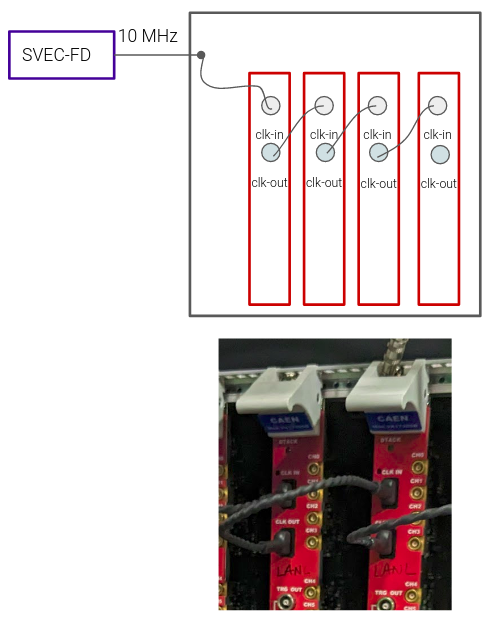
\includegraphics[width=\linewidth]{daisychain}
\caption{Daisy Chain}
\end{subfigure}
\hfill
\begin{subfigure}[h]{0.49\linewidth}
\centering    
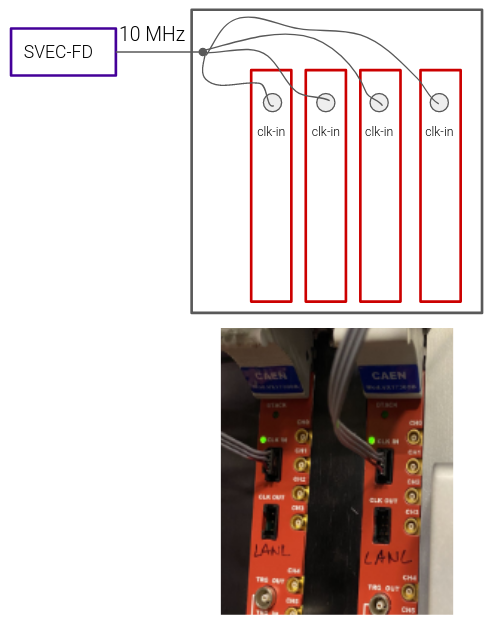
\includegraphics[width=\linewidth]{fanout}
\caption{Fan Out}
\end{subfigure}%
\caption[clockScheme]{
This diagram illustrates two different synchronisation clock schemes for the CAEN digitizers, daisy chain (left) and fan out (right).
}
\label{fig:clockScheme}
\end{figure}

\subsection{Evaluation of Timing Synchronisation}
\label{subsec42PMT}
Over the summer of 2023, the author has travelled to Fermilab for the second time to conduct the work on evaluating the timing resolution and synchronisation of the CAEN digitizers.
The first task was to determine which clock scheme to be used for physics run. 
The goal was to achieve synchronisation across all 8 CAEN digitizers and with respect the timing system of the DAQ.

%set up
The set up for the study consisted of 8 CAEN digitizers located in the same VME crate. 
Each digitizer received an identical signal into the TRG-IN connector directly from the PTB board, with the same cable length such that every digitizer was triggered simultaneously.
The trigger rate was set as 1 Hz.
To evaluate metric whether the CAEN digitizers are synchronised with each other, the timestamps of every triggered event from every digitizer should be identical with respect to each other. 

The trigger signal was also input to the SPEC-TDC for timestamping.
Timestamps of the trigger recorded by the CAEN digitizers and the SPEC-TDC can be compared against each other since both are referenced to the PPS signal.
The SPEC-TDC offers a higher level of precision compared to the CAEN digitizer.
Therefore, the comparison helps characterising the resolution of the timestamps produced the CAEN digitizer. 
This comparison also evaluates whether each CAEN digitizer is synchronised with respect to the PPS signal.

\begin{figure}[htbp!] 
\centering    
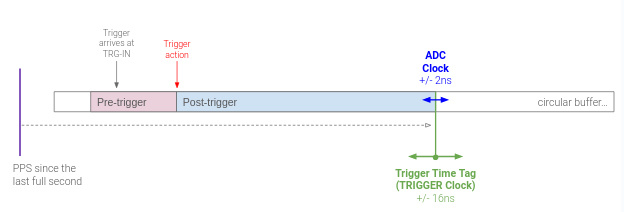
\includegraphics[width=1.0\textwidth]{TTT_diagram}
\caption[TTTDiagram]{
The diagram illustrate the how the CAEN digitizer constructs a Trigger Time Tag object upon receiving a trigger.
The timestamp embedded in the Trigger Time Tag accounts for a fixed buffer time the digitizer takes to generate the Trigger Time Tag upon receiving a trigger.
This timestamp also points the end the recorded waveform.
}
\label{fig:TTTDiagram}
\end{figure}

%CAEN Timestamp
In the previous section, the timestamps generated by the FEB module only needed adjustedment for cable lengths before being compared against the SPEC-TDC timestamps, since both the FEB modules and SPEC-TDC instantaneously generate timestamps upon receiving a trigger.
Meanwhile, the CAEN digitizer generates a timestamp object called TTT associated with every trigger, and this timestamp is not instantaneous upon the trigger arrival time, as illustrated in Fig. \ref{fig:TTTDiagram}. 
Upon receiving a trigger at the TRG-IN connector, the digitizer has a fixed buffer time before the trigger action occurs and generates a TTT.
The generated TTT also points to the end of the waveform, such that it is the timestamp value of the last tick on the waveform.
Therefore, to ensure consistency in comparing the timestamps of the CAEN digitizer and the SPEC-TDC, they need to be corrected to the same reference frame, which was chosen to be the time at which the trigger leaves the PTB front face.
If both the CAEN digitizers and the SPEC-TDC synchronised with each other, the difference in the timestamps should be 0.

\begin{figure}[htbp!]
\begin{subfigure}[h]{1.00\linewidth}
\centering    
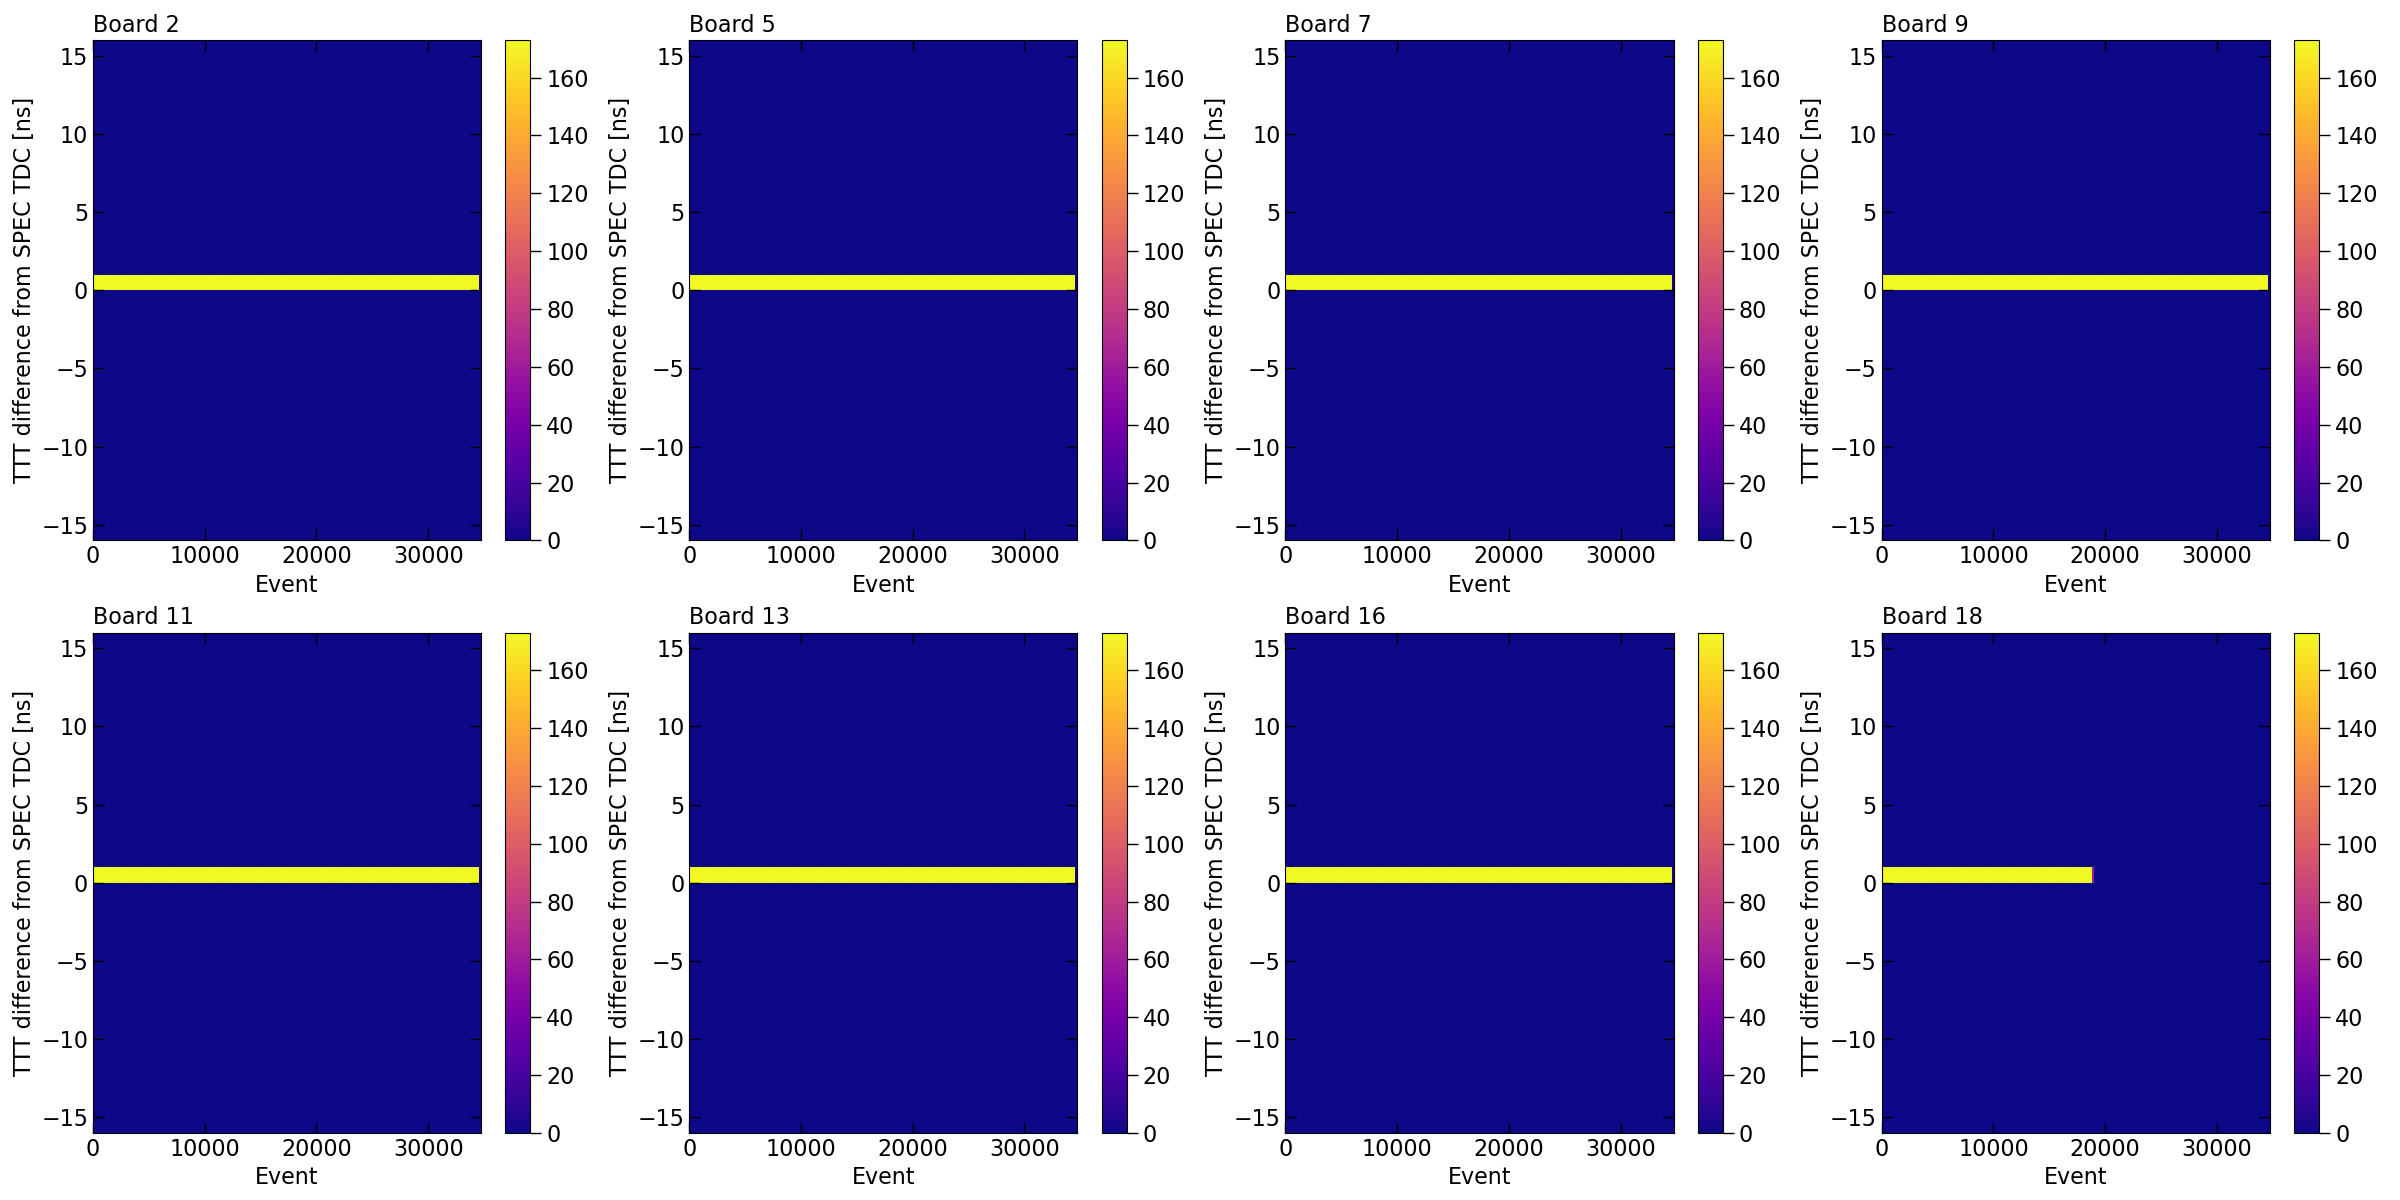
\includegraphics[width=\linewidth]{TTT_SPEC_diff_run7980}
\caption{Run7980}
\end{subfigure}
\hfill
\begin{subfigure}[h]{1.00\linewidth}
\centering    
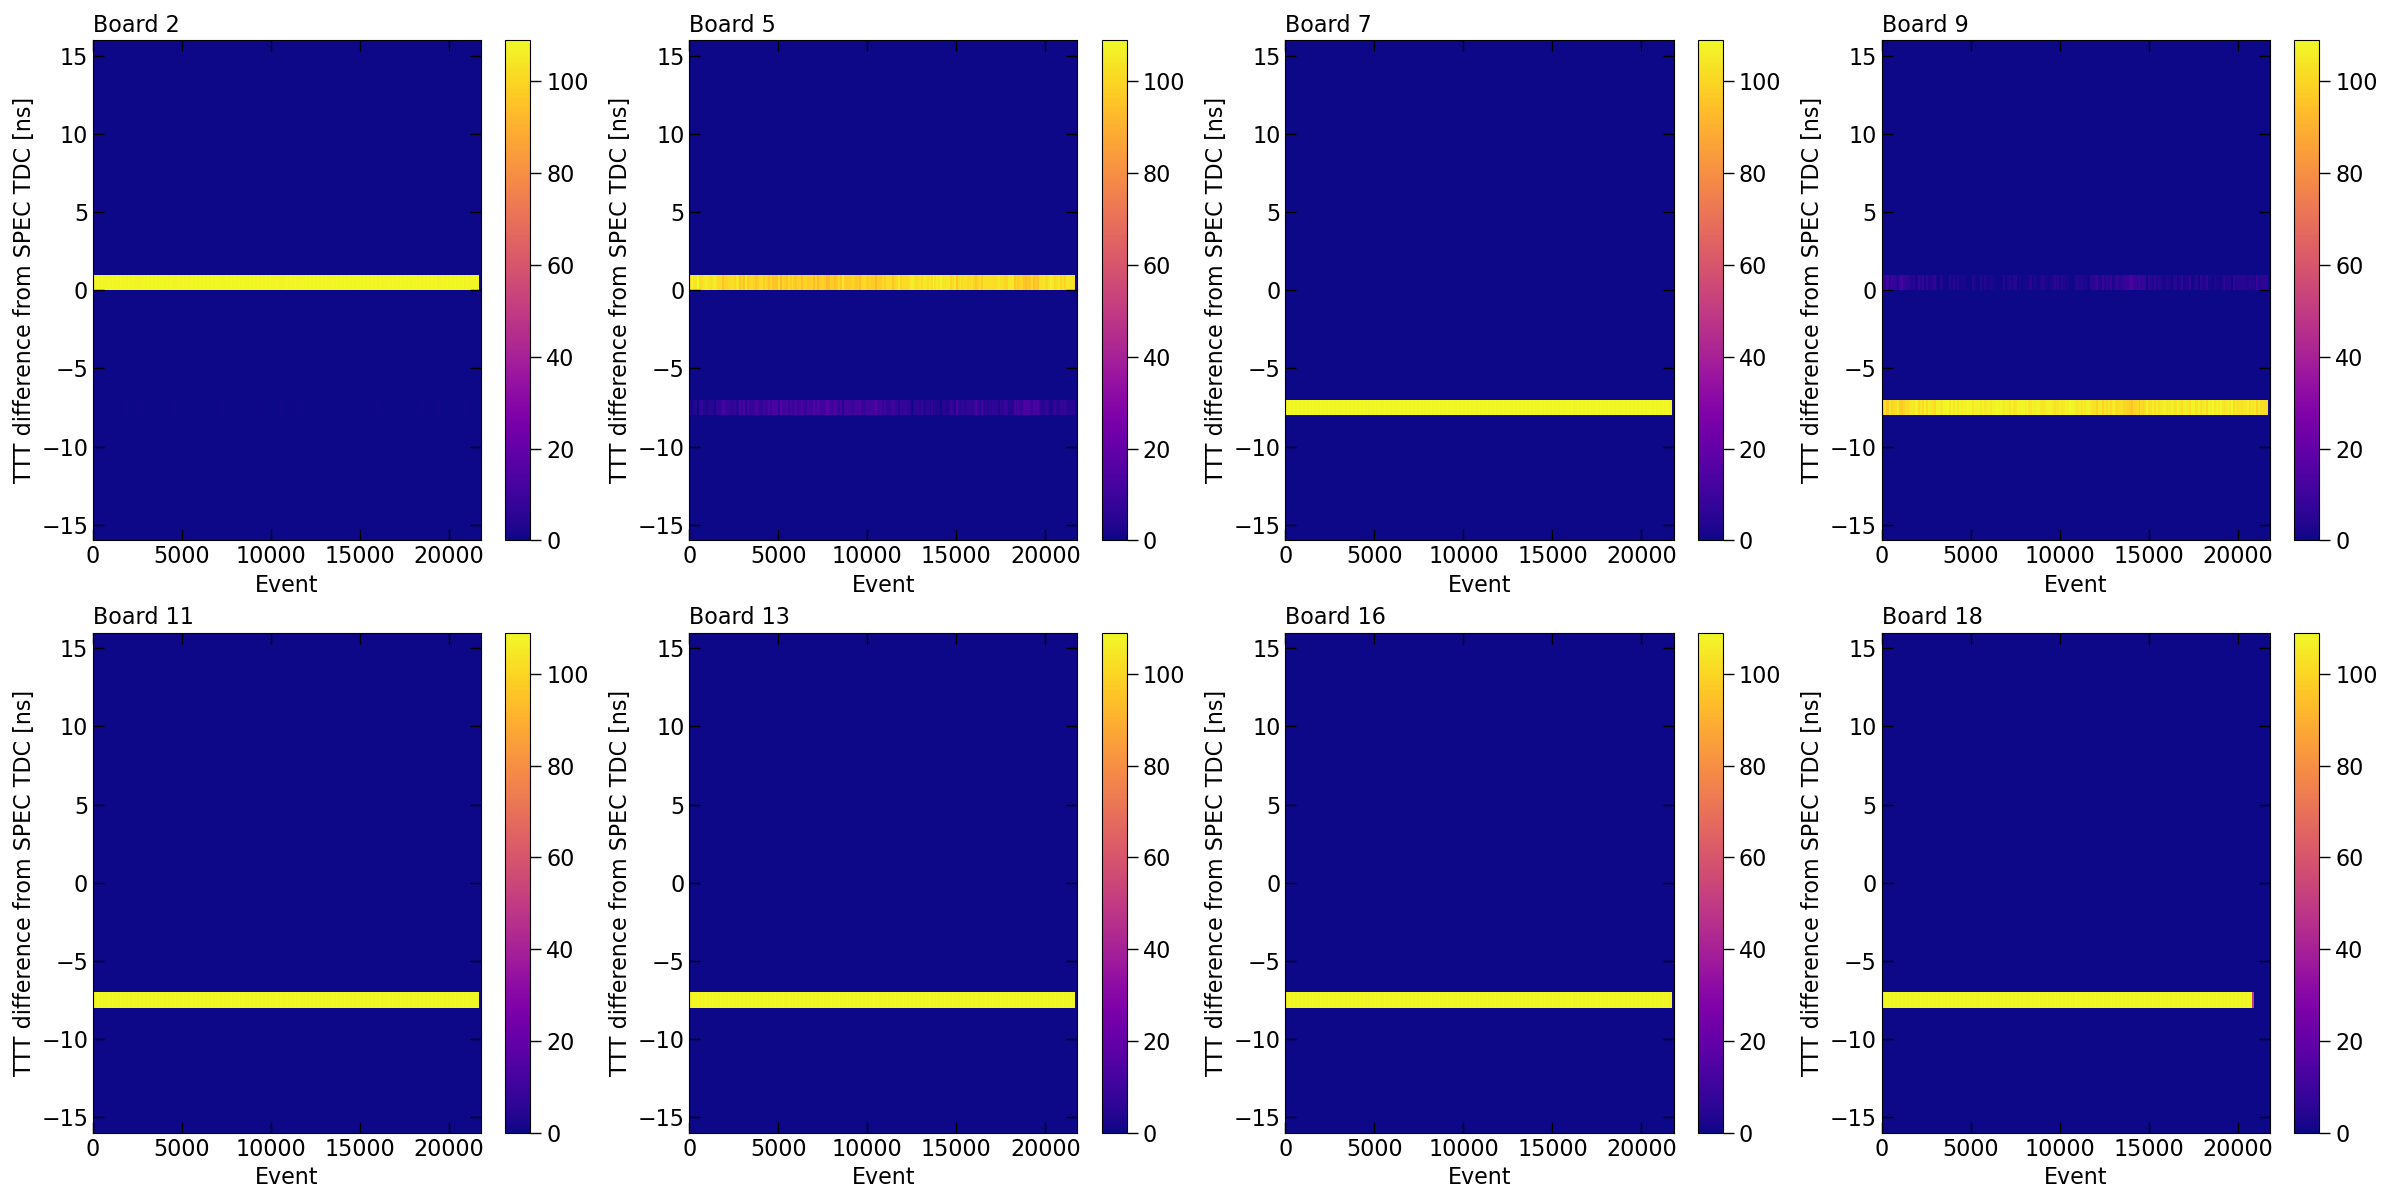
\includegraphics[width=\linewidth]{TTT_SPEC_diff_run8060}
\caption{Run 8060}
\end{subfigure}%
\caption[daisychainSPEC]{
The comparison of the timestamps produced by the CAEN digitizer against those produced by the SPEC-TDC with the CAEN digitizers employing the daisy chain clock scheme.
Run 7980 shows perfect synchronisation whilst run 8060 shows the effect of clock drifting in a daisy chain clock scheme.
}
\label{fig:daisychainSPEC}
\end{figure}

%Result from daisy chain
The daisy chain clock scheme underwent testing across multiple DAQ runs over a few days. 
An example of the results is shown in Fig. \ref{fig:daisychainSPEC} for run 7980 and run 8060.
The results for run 7980 demonstrates perfect synchronisation across all 8 CAEN digitizers, as well as synchronisation with respect to the SPEC-TDC, and thus the PPS signal.
All the timestamps agree within a single nanosecond and remain stable during the full run.
In contrast, run 8060 was taken 4 days after run 7980 and exhibited interesting effects.
Board 7 in the daisy chain drifted by 8 ns, causing all subsequent boards in the daisy chain to also drift, yet they remained synchronised with each other. 
Moreover, board 5 also shows a straddling effect, resulting in a jittering of 8 ns.
This straddling behaviour is expected since the trigger clock of CAEN digitizer is read every 2 clock cycles, introducing fluctuations twice the tick value of 8 ns.
Both these runs also show that board 18 stopped taking data a while into the DAQ run, which was found to be due to a malfunctioning temperature sensor in this CAEN digitizer.
This digitizer was sent away to the manufacturer for repair.

\begin{figure}[htbp!]
\begin{subfigure}[h]{1.00\linewidth}
\centering    
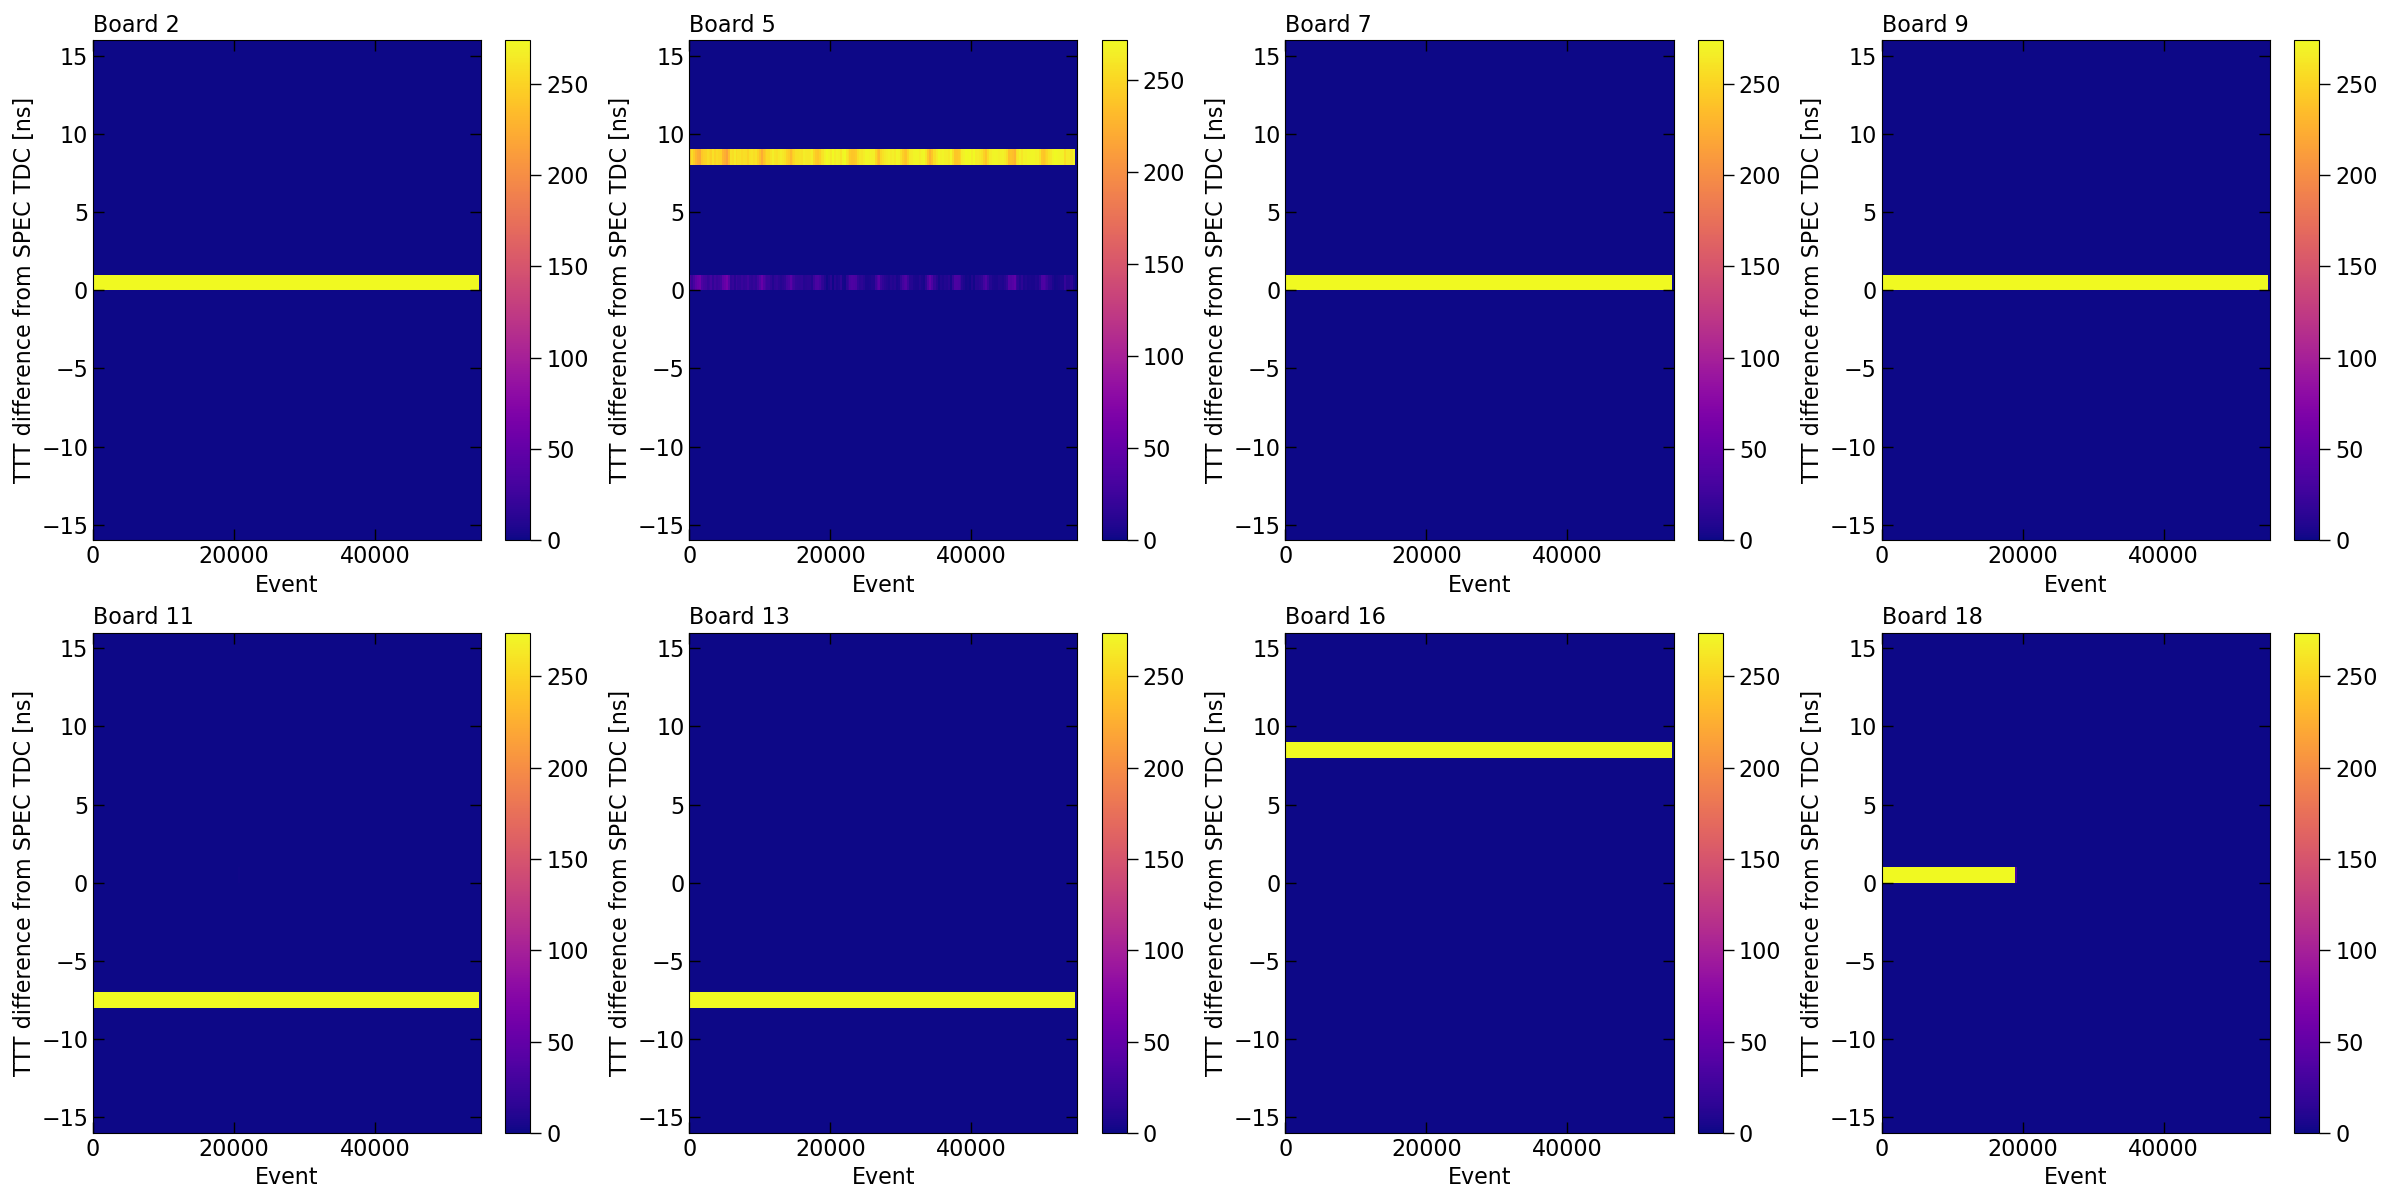
\includegraphics[width=\linewidth]{TTT_SPEC_diff_run8178}
\caption{Run8178}
\end{subfigure}
\hfill
\begin{subfigure}[h]{1.00\linewidth}
\centering    
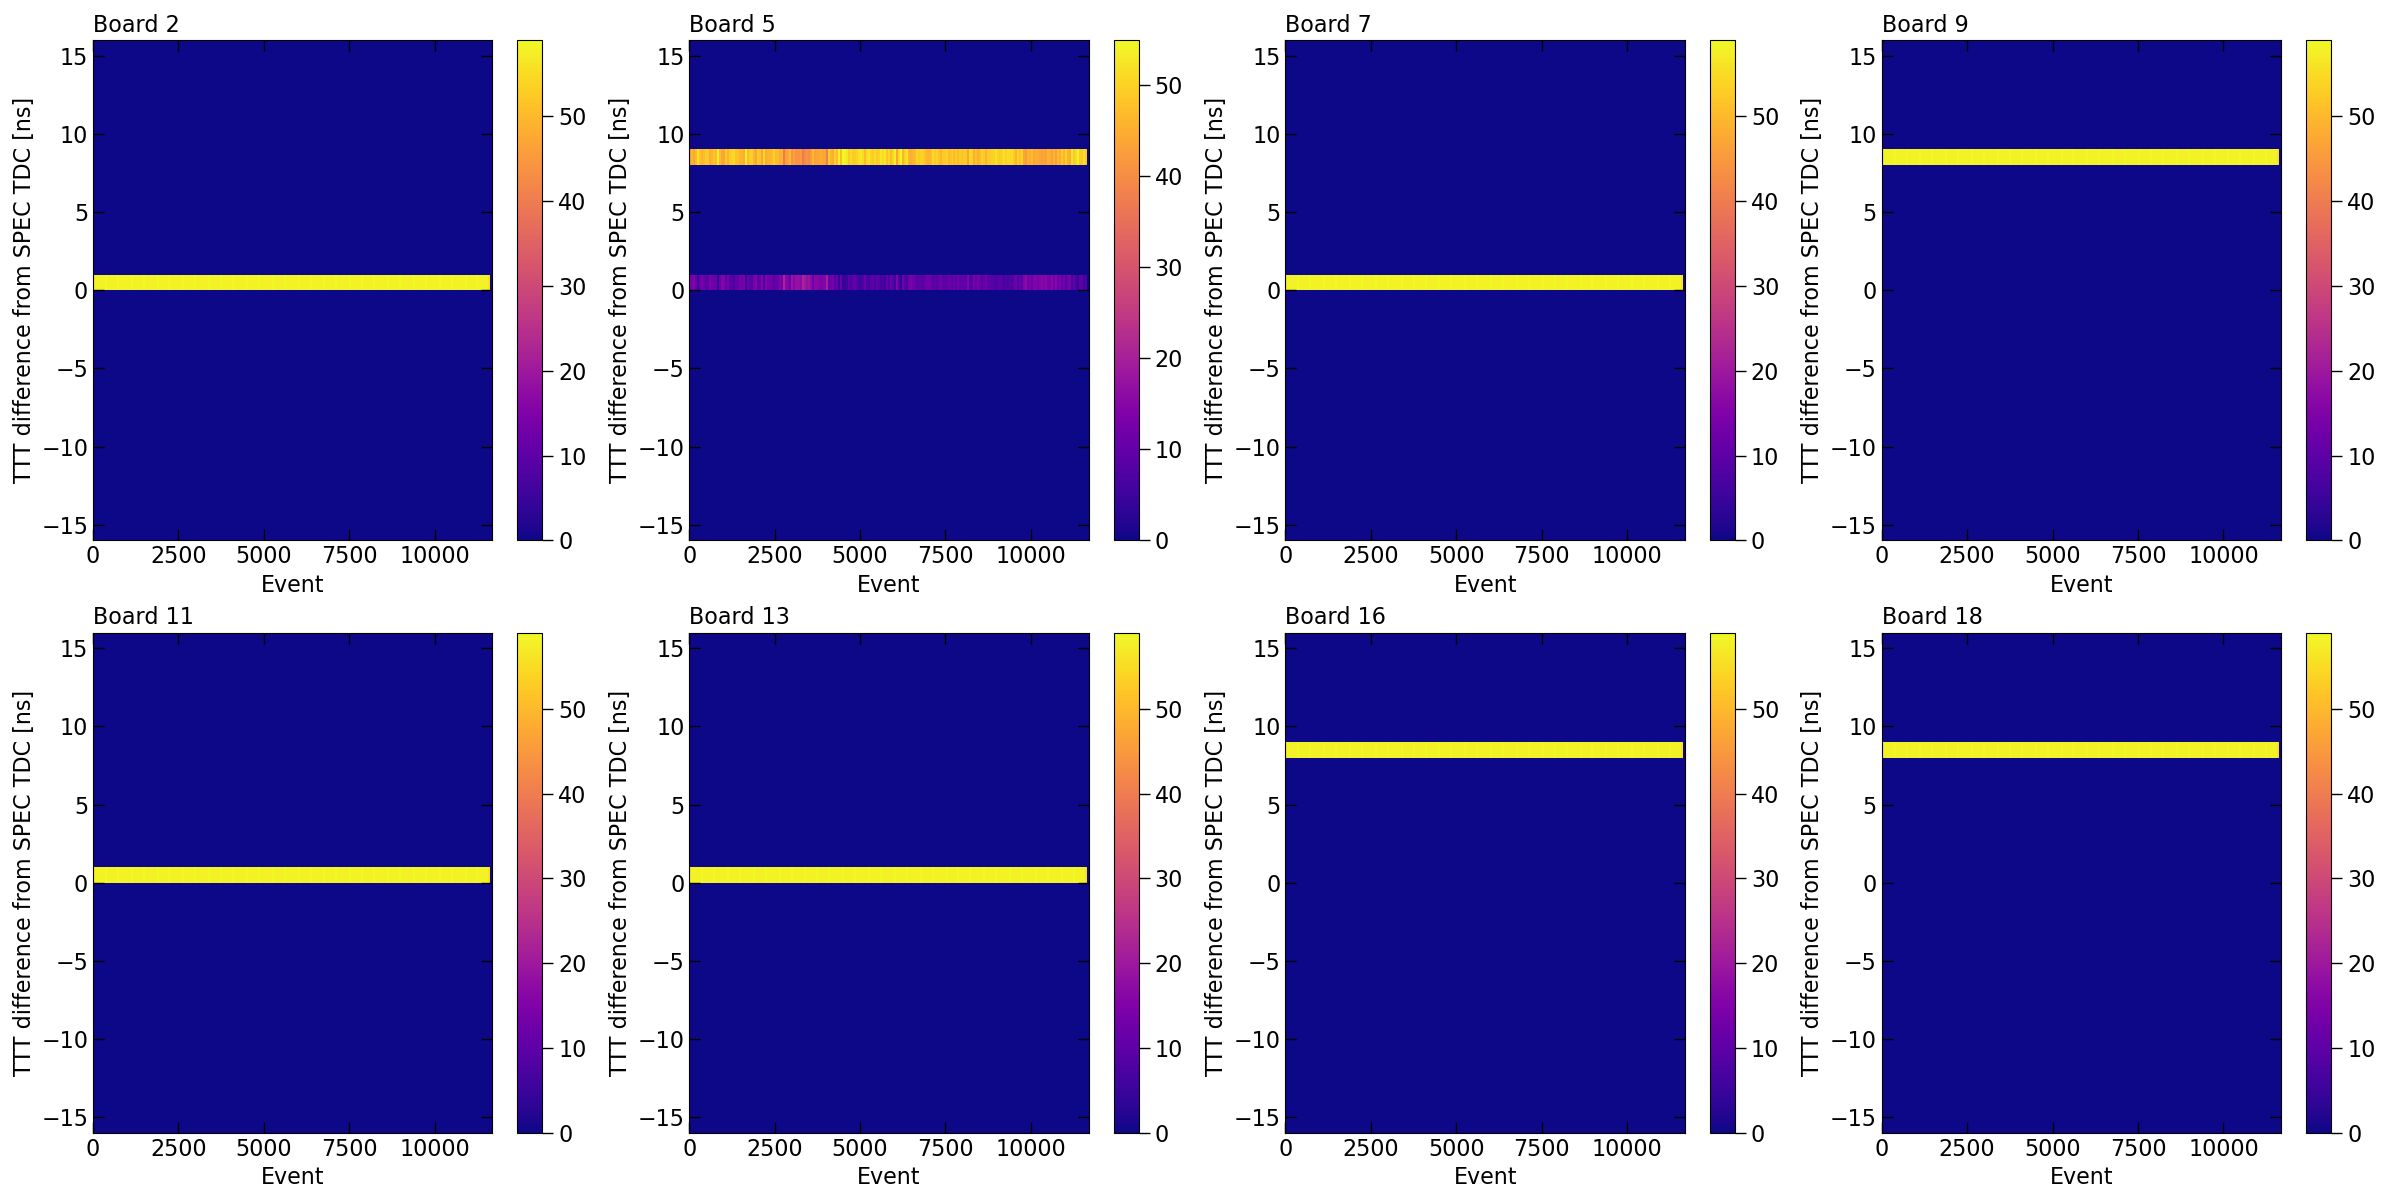
\includegraphics[width=\linewidth]{TTT_SPEC_diff_run8196}
\caption{Run 8196}
\end{subfigure}%
\caption[fanoutSPEC]{
The comparison of the timestamps produced by the CAEN digitizer against those produced by the SPEC-TDC with the CAEN digitizers employing the fan out clock scheme.
Since the input frequency of 10 MHz is not phase with the trigger clock frequency of 125 MHz, this introduces a random phase offset in timestamps across all the digitizers and different runs. 
}
\label{fig:fanoutSPEC}
\end{figure}

%Result from fan out
The same test was repeated for the fan out clock fan scheme, where multiple DAQ runs were conducted over a few days.
An example of the run results is shown in Fig. \ref{fig:fanoutSPEC} for run 8178 and run 8196.
In both of these runs, board 5 shows the same straddling effect, causing timestamps to jitter by 8 ns.
One key difference in this clock scheme is that the timestamps recorded by each CAEN digitizer varies randomly between digitizers and across different runs. 
This variation is due to the input frequency to the CLK-IN connector set at 10 MHz.
As previously explained, the trigger clock is generated by the AD9510 chip, which must be in phase with the input frequency. 
However, the trigger clock operates at a frequency of 125 MHz, while the input frequency remains at 10 MHz. 
Since these frequency values are not multiples of each other, they do not agree in phase.
To generate an out-of-phase frequency, the AD9510 chip latches onto the first rising edge of the input frequency upon the digitizer initialisation. 
Consequently, when the CAEN digitizer is initialised at the beginning of every DAQ, a random phase offset is introduced, causing the timestamps to vary from run to run.
Moreover, the 10 MHz clock is distributed in fan out scheme to every digitizer resulting in the phase offset varies randomly from one digitizer to another.

%settle for daisy chain over fan
Comparing between the two clock schemes, the daisy chain mode offers better synchronisation across the 8 CAEN digitizers compared to the fan out mode.
In the daisy chain scheme, only the first CAEN in the daisy chain receives the external 10 MHz clock.
The master clock CAEN digitizer can have a random phase offset that propagtes down the daisy chain, resulting in synchronisation across all digitizers.
However, it is important to note that the clock drift effect has been observed while testing the daisy chain scheme
Monitoring these effects during the commissioning period is necessary to understand the impacts of the clock drift."

\subsection{Clock Jittering Correction}

To further characterise the timing resolution of the CAEN digitizer, an additional test was added to understand how precisely the board digitizes the waveform.
As demonstrate in Fig. \ref{fig:TTTDiagram}, the TTT object is the timestamp of the last tick of waveform, and thus, this provides the timing information to construct the timing of the waveform.
From the manuals of the digitizer, it is indicated that the trigger clock and the ADC sampling clock are synchronised with respect to each other.
Thus, this test aimed to test whether all 8 CAEN digitizers can digitize waveform in synchronisation with each other within a nanosecond. 

\begin{figure}[htbp!] 
\centering    
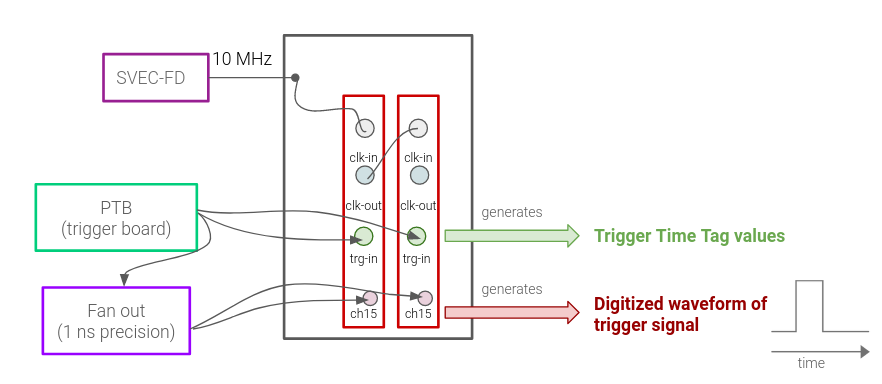
\includegraphics[width=1.0\textwidth]{digitize_ftrig}
\caption[digitizeFTRIG]{
The set up for study the synchronisation of the CAEN digitizers and their timing resolution.
In this set up, the 1 Hz trigger is produced from the PTB, and input into the TRG-IN channel of each CAEN for simultaneous triggering.
The timestamp of the trigger is embedded in the Trigger Time Tag object.
The trigger is also propagate to a fan out module, and input into channel 15 of every CAEN digitizer.
The waveform of the trigger signals is expected to be digitized simultaneously. 
}
\label{fig:digitizeFTRIG}
\end{figure}

%setup
This study used the same set up as described in the previous section.
An additional setup was to input the trigger into channel 15 of every CAEN digitizer with the same amount of cable length so that all triggers would be digitized simultaneously as shown in Fig. \ref{fig:digitizeFTRIG}.
In this configuration, the trigger would be timestamped in the TTT object, as well digitized as a waveform. 

%two different modes to compare timestamp
This set up presents two types of timestamps produced by the CAEN digitizer.
As illustrated in Fig. \ref {fig:TTTDiagram}, one timestamp is derived from the TTT value produced by the trigger clock of the CAEN digitizer.
These timestamps were examined in the synchronisation study in section \ref{subsec42PMT}.
This type of timestamp is now referred as the TTT-derived timestamp.
Given that the waveform of the trigger signal is now digitized, one can determine the rising edge of the trigger signal.
This gives a tick value on the waveform and thus, the timestamp associated to this tick which can be derived from the TTT value.
This type of timestamp is referred as the tick-derived timestamp, since this timestamp requires the knowledge of the tick position of the trigger on the waveform as well as the TTT value.
Both these timestamps are compared against the SPEC-TDC timestamps of the trigger signals, to the same reference frame at which the trigger leaves the PTB front face.
Cable length corrections were also applied.

\begin{figure}[htbp!] 
\centering    
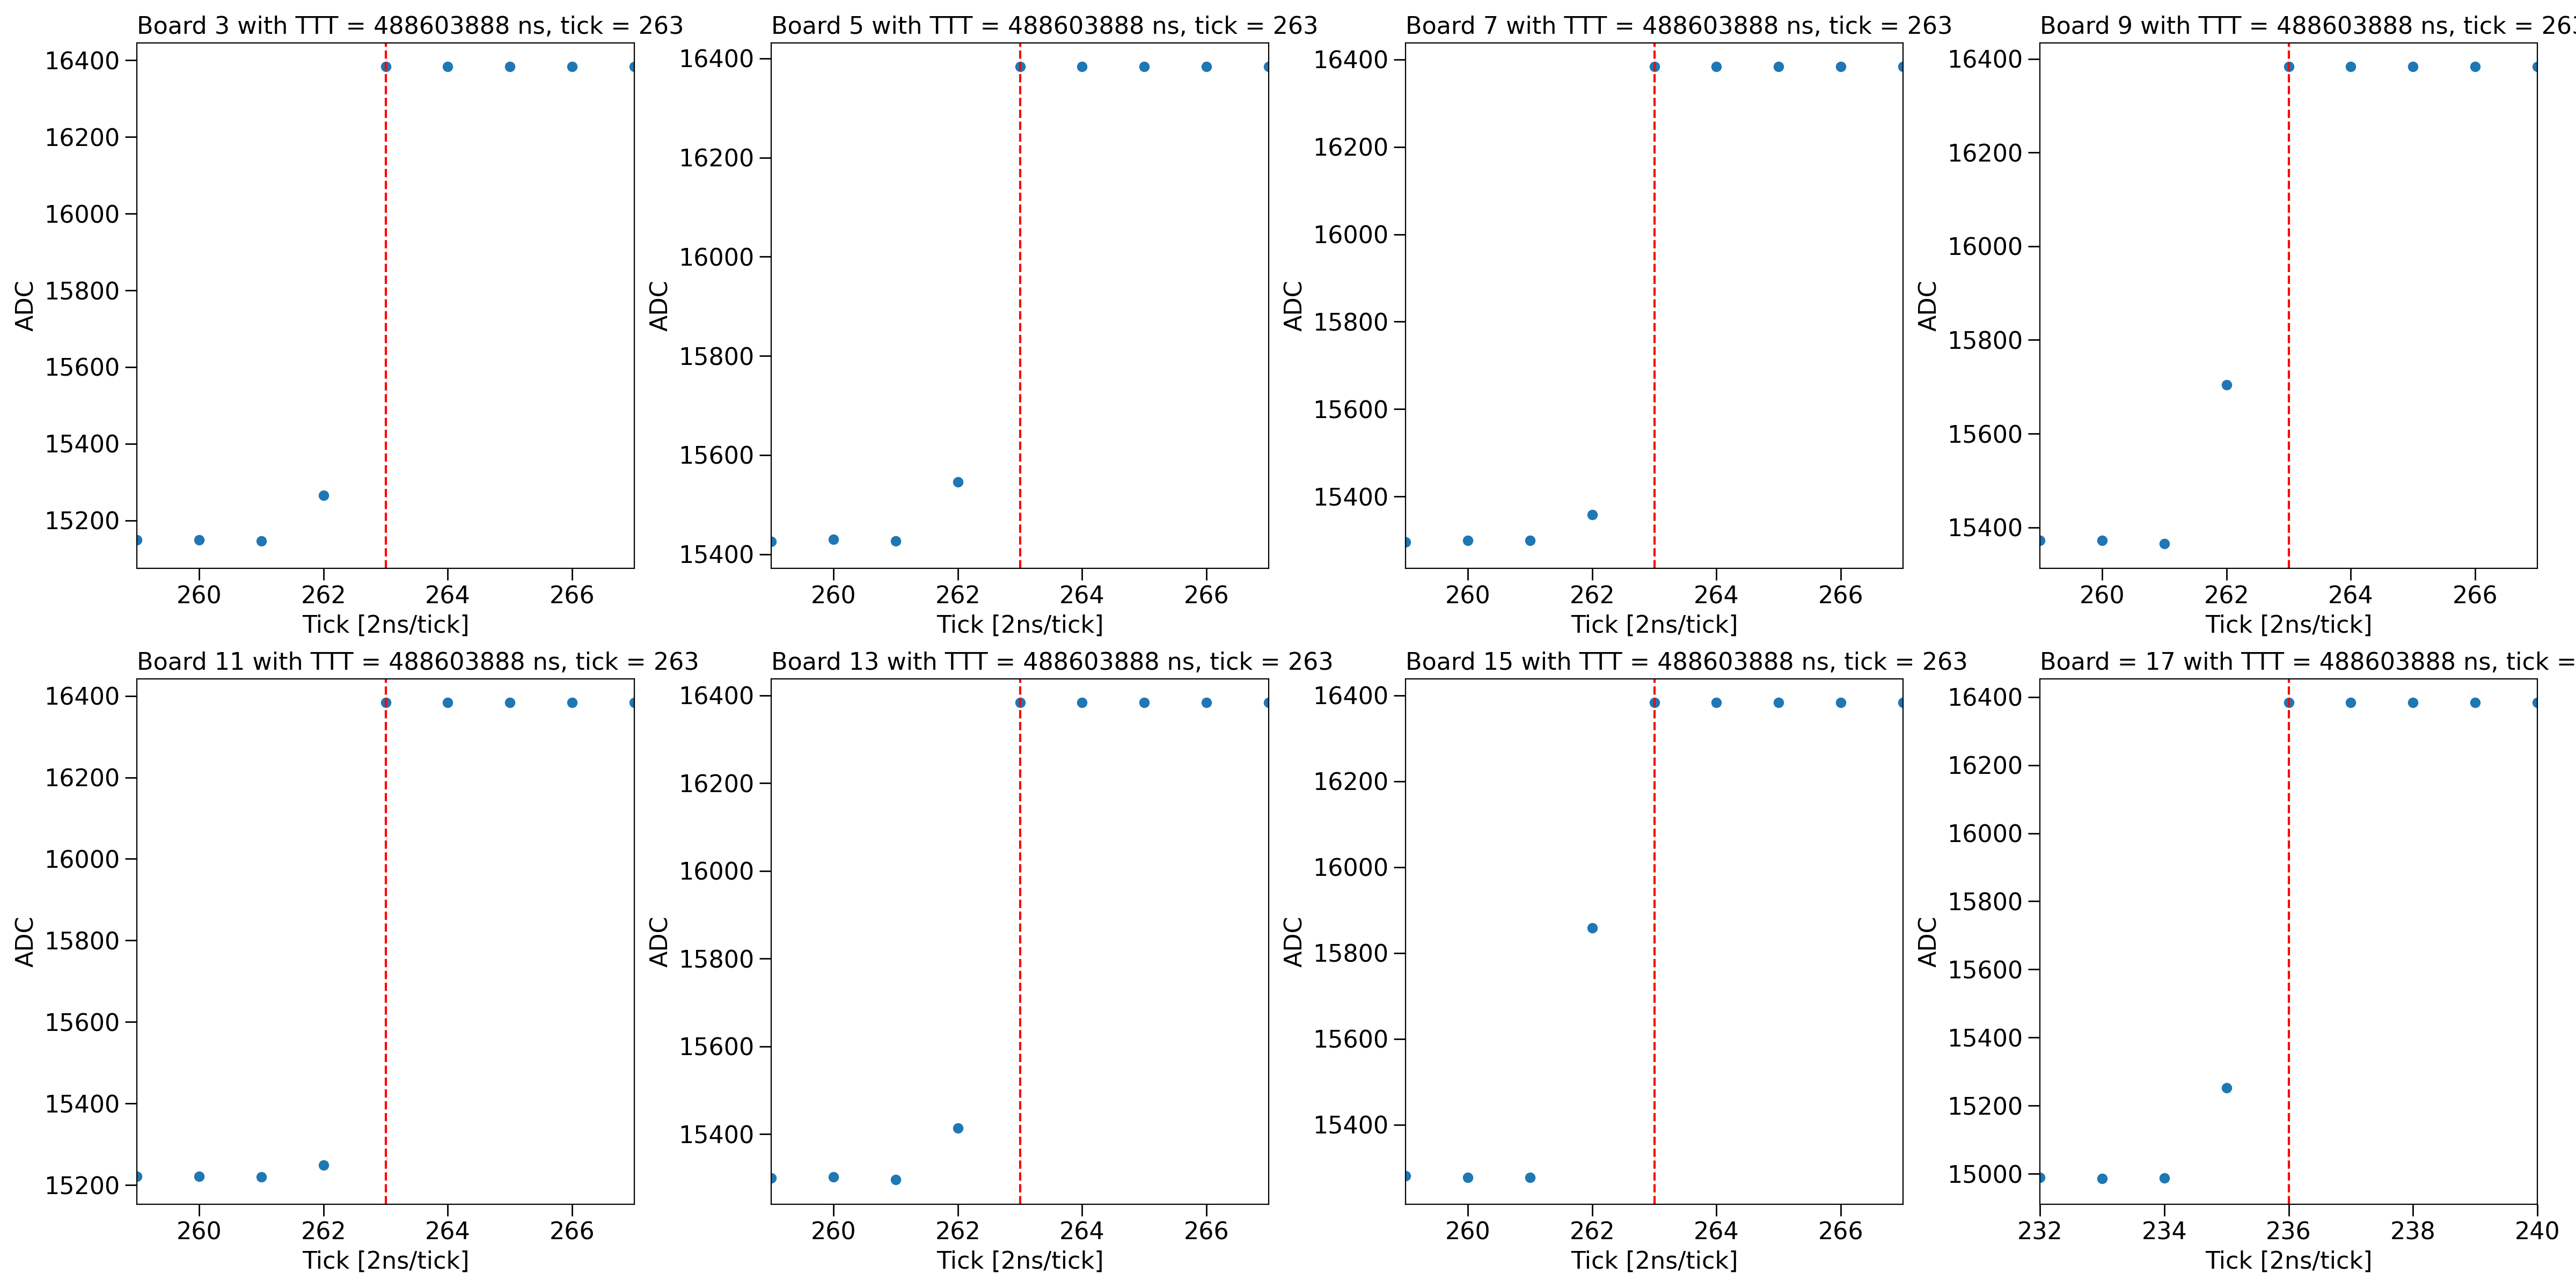
\includegraphics[width=1.0\textwidth]{daisychain_calib}
\caption[daisychainCALIB]{
After the daisy chain calibration, the waveforms of the simultaneous triggers are plotted to check for synchronisation.
The TTT values associated with the each waveform are identical, showing that the digitizers receive triggers at the same time.
The waveforms of the triggers are zoomed around the rising edge, showing the identical tick value of the rising edge, showing that all the boards also digitize the trigger at the same time.
Board 17 is an exception because it has a different firmware compared to the rest of the digitizers and digitizes the waveform slightly different.
}
\label{fig:daisychainCALIB}
\end{figure}

The daisy chain clock scheme was also re-calibrated before conducting this study.
As described in section \ref{subsec41PMT} on the overview of the CAEN digitizer clock, the clock propagation from the master clock to the slave clock needs to be delayed with a precise amount such that their clocks are exactly in phase.
This calibration process was to ensure that not only every digitizer would produce identical timestamps for simultaneous triggers, but also would digitize the trigger signals simultaneously.
The result after the process is demonstrated in Fig. \ref{fig:daisychainCALIB}, showing that every digitizer has the same timestamp and digitizes the trigger signal at the exact same tick position on the waveform.As a result, the timestamps of the tick value on the rising edge of trigger signals, or the tick-rived timestamps, are identical across all 8 CAEN digitizers.

Multiple DAQ runs were taken for this study over a period of one month.
Each run duration varied from less than an hour up to 10 hours.
The purpose of this was also to test the stability of the synchronisation of the daisy chain and its impact on the resolution of the produced timestamps.
This timing resolution study was conducted on a dataset of 30 runs.

\begin{figure}[htbp!]

\begin{subfigure}[h]{1.00\linewidth}
\centering    
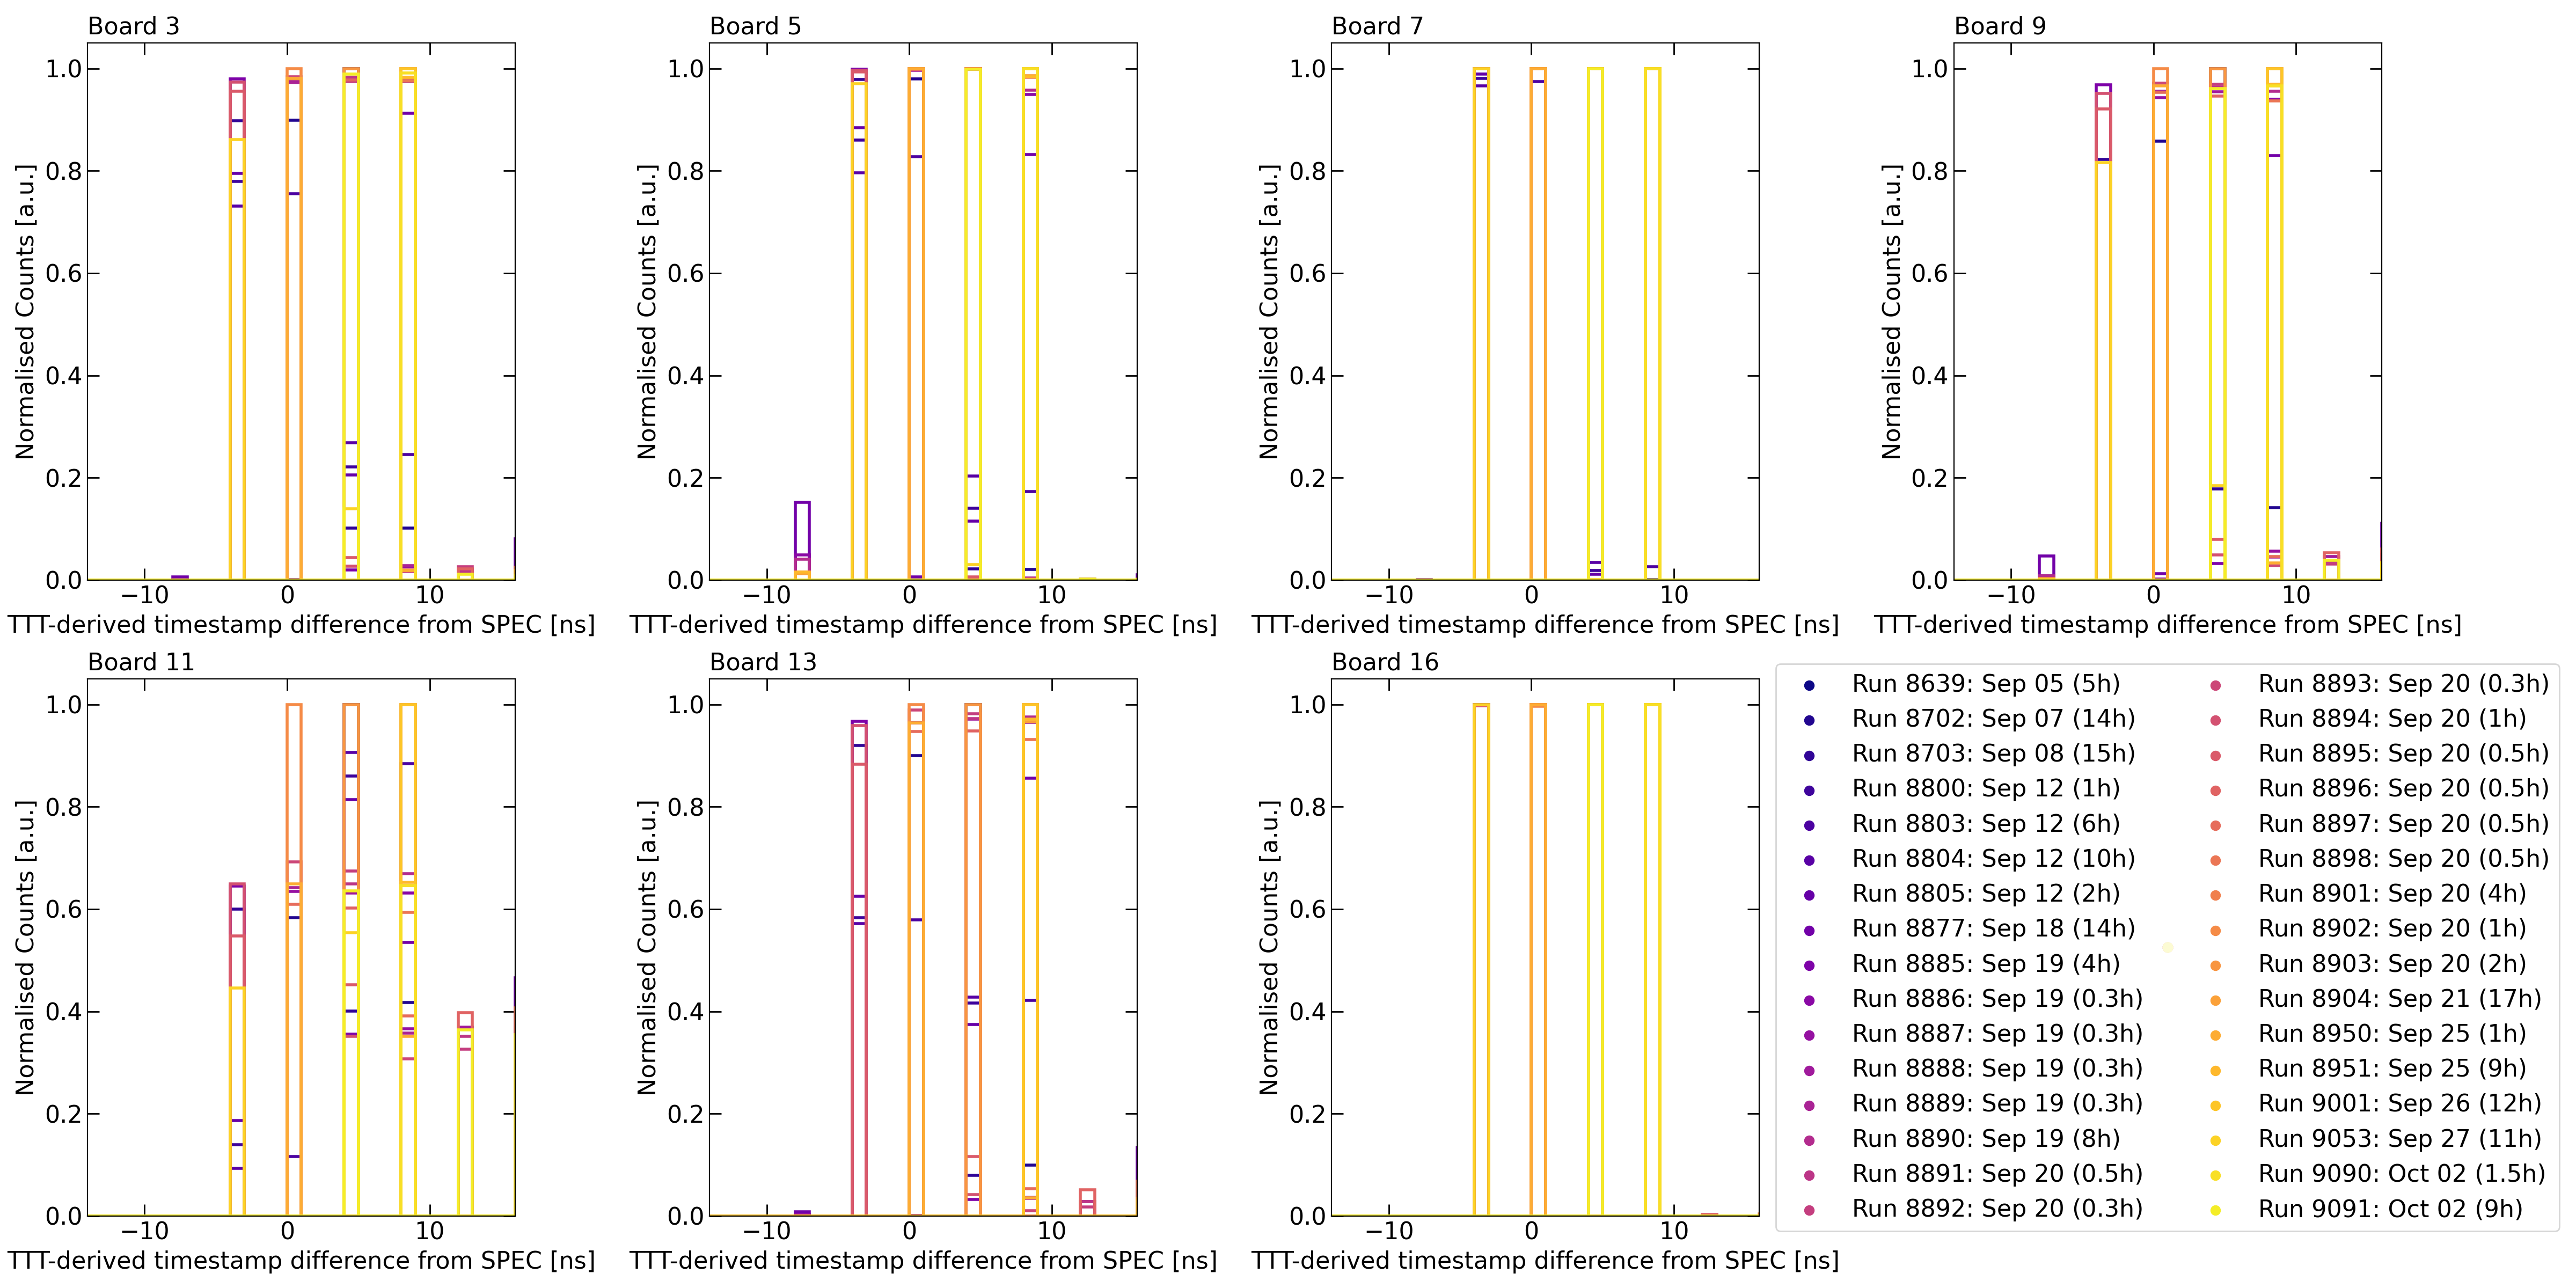
\includegraphics[width=\linewidth]{TTTts_spec}
\caption{TTT-derived timestamps}
\label{subfig:TTTts_spec}
\end{subfigure}

\hfill
\begin{subfigure}[h]{1.00\linewidth}
\centering    
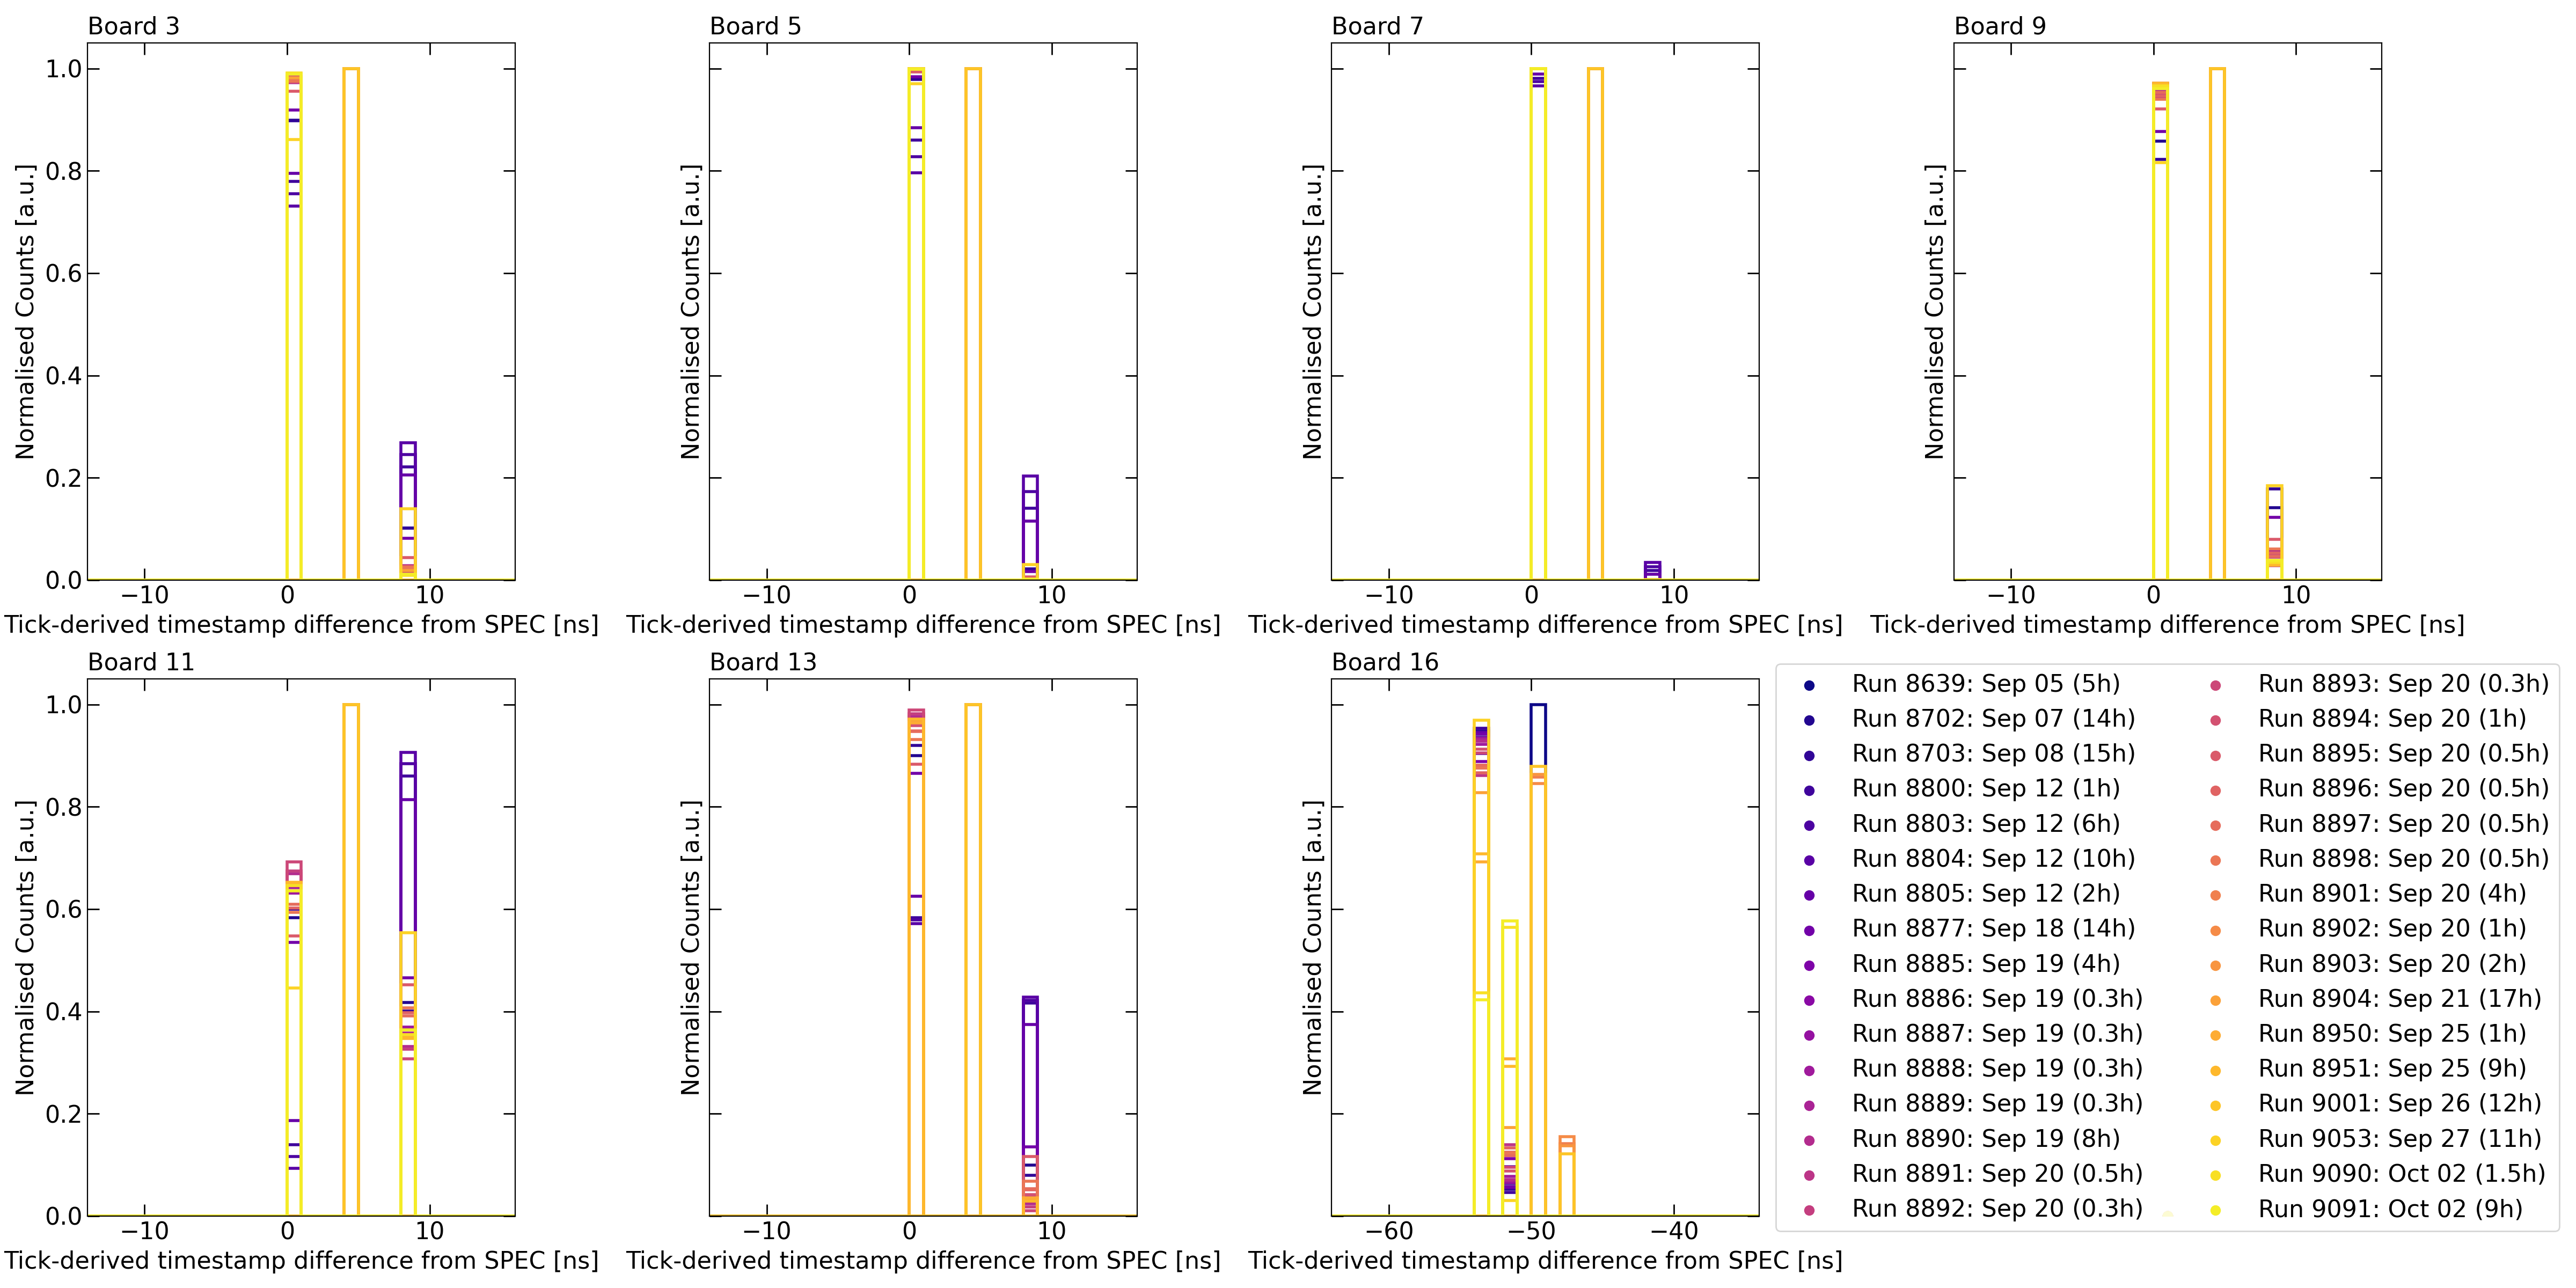
\includegraphics[width=\linewidth]{Tickts_spec}
\caption{Tick-derived timestamps}
\label{subfig:Tickts_spec}
\end{subfigure}%

\caption[TTTtsTickts]{
The two timestamps distributions generated by the CAEN digitizers, compared against the SPEC-TDC timestamps.
The TTT-derived timestamps show a large spread up to 24 ns whilst the Tick-derived timestamps show a much smaller spread of only 8 ns.
}
\end{figure}

%TTT timestamps
The TTT-derived timestamps distribution is plotted in Fig. \ref {subfig:TTTts_spec} for 7 CAEN digitizers, compared against the SPEC-TDC timestamps.
This distribution shows a large spread up to 24 ns, which indicates that TTT-derived timestamp has a variation larger than what is stated in the manuals, that the trigger clock resolution is 16 ns.
The tick-derived timestamps distribution is plotted in Fig. \ref {subfig:Tickts_spec}.
This distribution, however, shows a much small spread of only 8 ns.

To understand the differences between the two types of timestamps, the tick position of the rising edge of the trigger waveform is also plotted in Fig. \ref {fig:TickSPEC}.
The distribution shows a large spread up to 5 ticks, equivalent to 10 ns.
This illustrates that the CAEN digitizer does not consistently digitize the trigger waveform, causing variations in the tick position of the rising edge between different events, run and digitizers.
This implies that not only can the trigger clock of the CAEN digitizer jitter, but its ADC sampling clock can also fluctuate, potentially introducing additional smearing.

\begin{figure}[htbp!]
\centering    
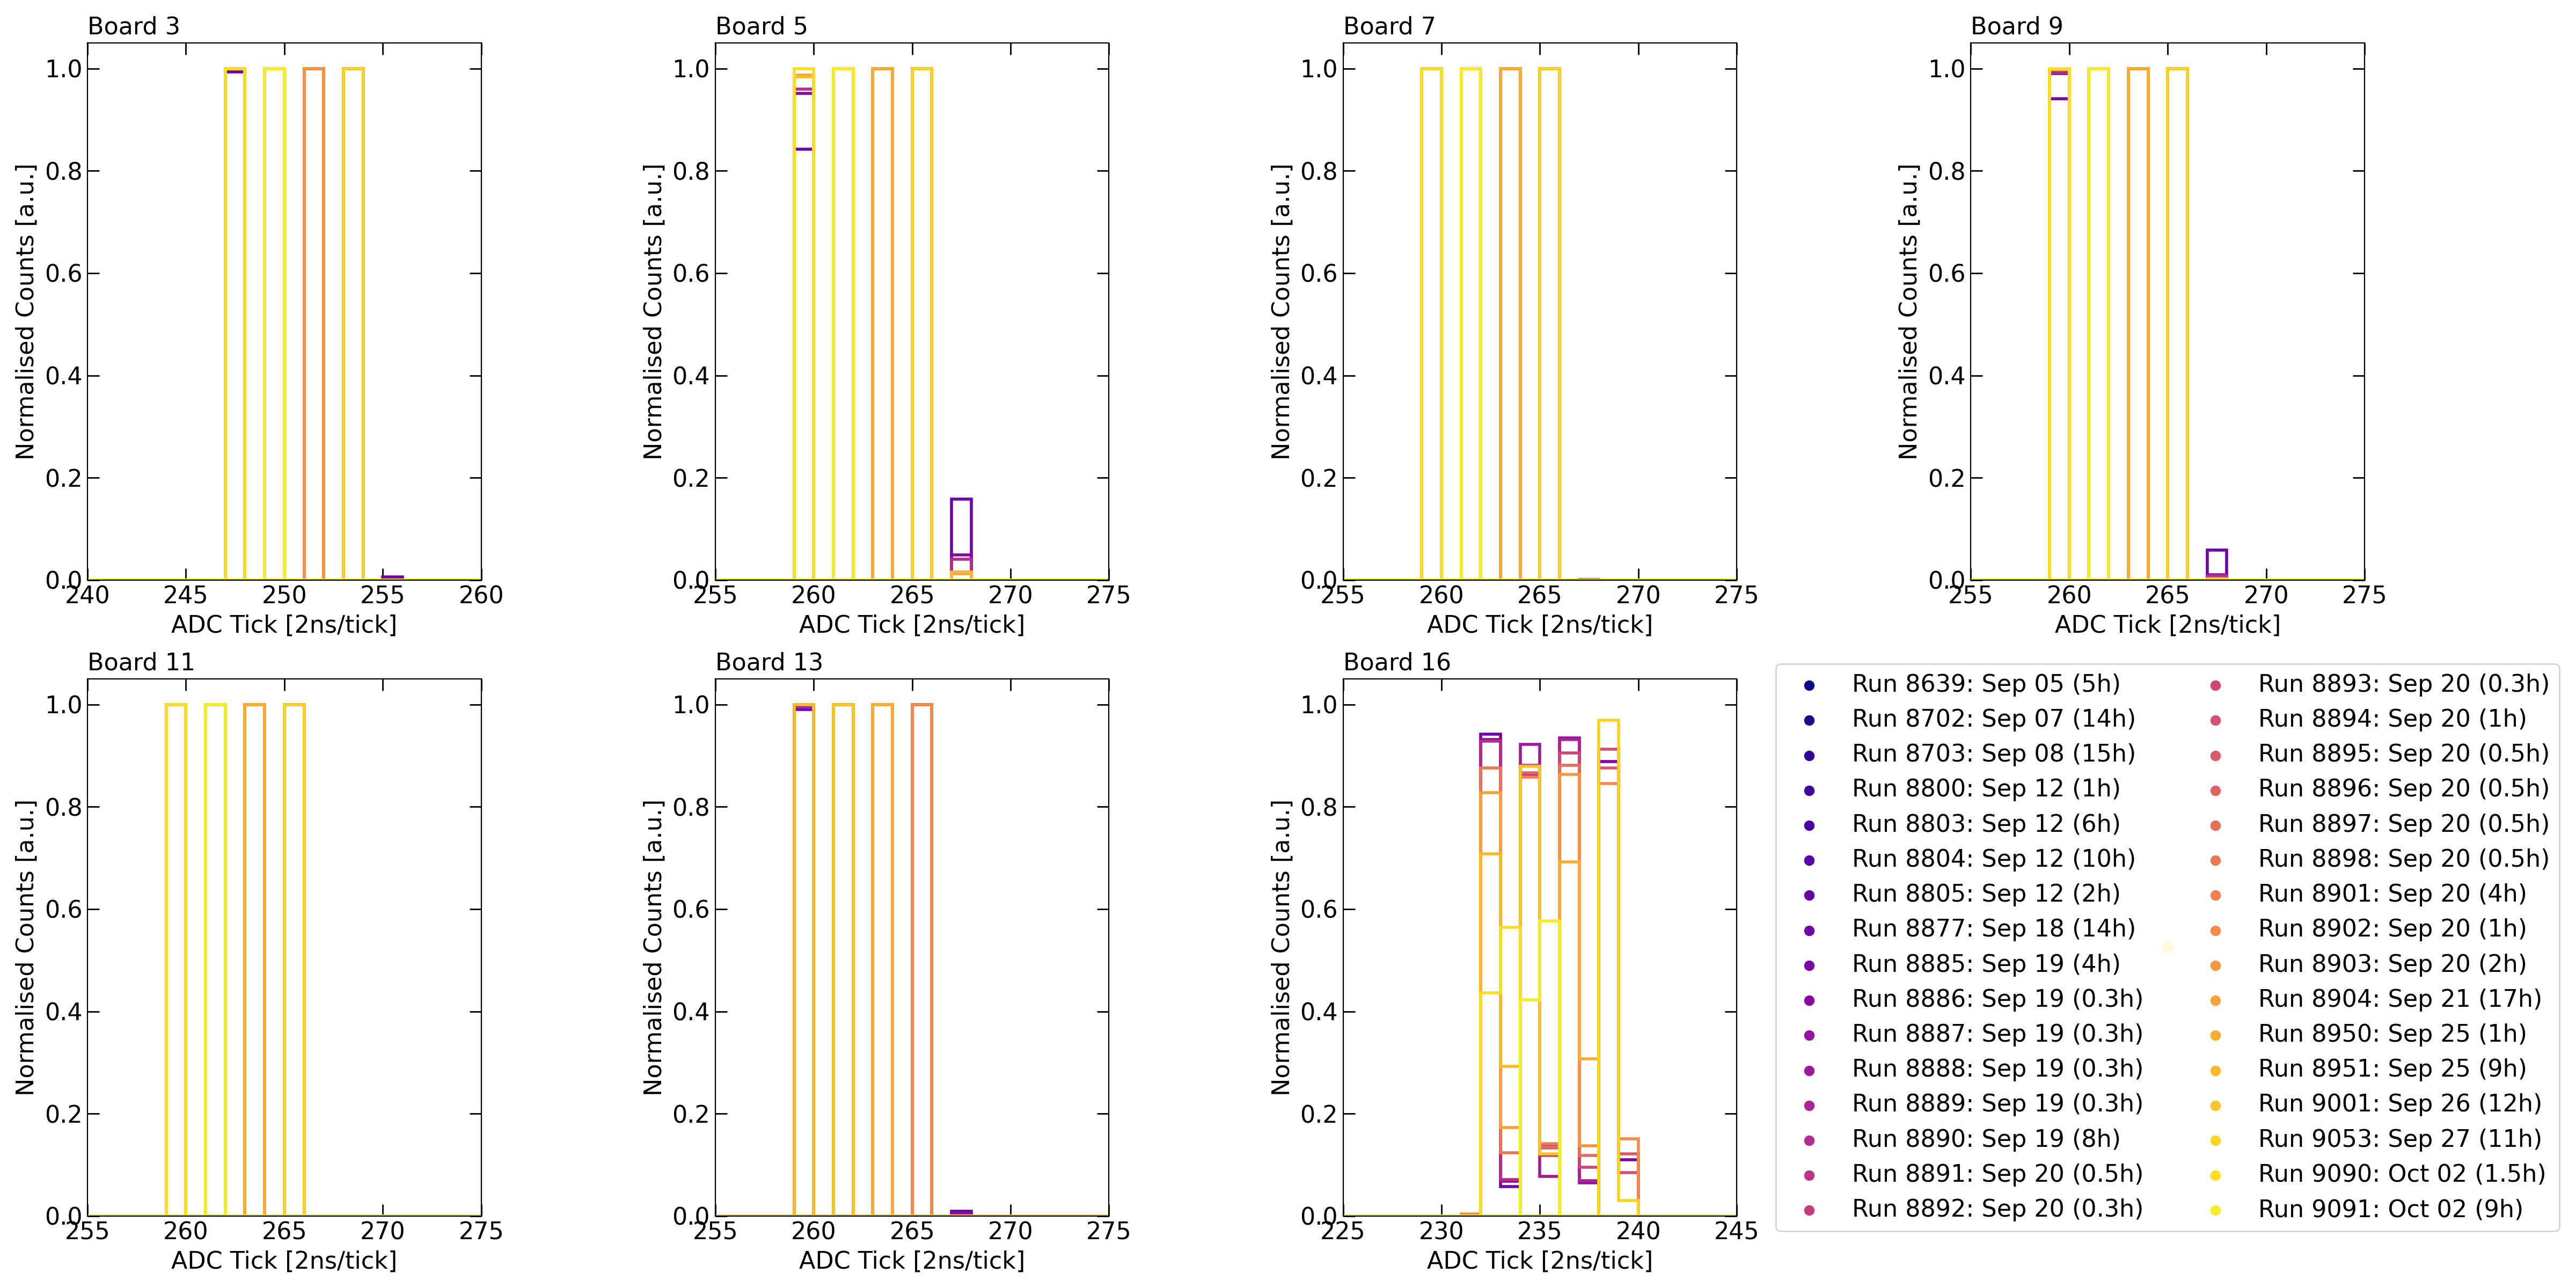
\includegraphics[width=\linewidth]{Tick_spec}
\caption[TickSPEC]{
The distribution of the tick value of the rising edge of the trigger waveforms has variation up to 5 ticks, equivalent to 10 ns. 
This demonstrates that the ADC sampling clock of the CAEN digitizer can also jitter.
}
\label{fig:TickSPEC}
\end{figure}

The CAEN manuals highlight that the trigger clock and the ADC sampling clock are correlated to each other, and this is reflected in the fact that the TTT value points to the last tick of the wave form.
The CAEN digitizer was designed on purpose to have the trigger clock in synchronised with the ADC sampling clock, so that the trigger clock can track and absorb the jittering of the ADC sampling clock.
This explains the 24 ns spread of the TTT-derived timestamps since it contains the smearing from both the trigger and the ADC sampling clocks.
Meanwhile, the tick-derived timestamps distribution shows a much smaller spread of 8 ns, since tht timestamp was produced using both the TTT value and tick value, resulting in a high level of precision.

%jittering cases
This understanding of the clock behaviour of the CAEN digitizer opens up venues for correcting for the timestamp jittering.
The tick-derived timestamp dataset were further examined in order to understand how to apply the correction to completely remove the 8 ns spread.
Three cases of jittering were identified and illustrated in Fig. \ref{subfig:jitter_before},  
The first case occurs when the ADC sample can jitter whilst the triggering clock remains stable.
This results in a different tick value of the rising edge, and introduces a tick-derived timestamp is smeared out by the ADC sampling clock tick value of 2 ns.
In the second case, the opposite situation arises such that the tick value of the rising edge is stable however the trigger clock jitters in step of 8 ns, resulting in the smearing of tick-derived timestamp by the same amount.
The last case is the combination jittering from both clocks, such that the smearing amount is a sum of the trigger and ADC sampling clock tick value, equal to 10 ns.

\begin{figure}[htbp!]

\begin{subfigure}[h]{1.00\linewidth}
\centering    
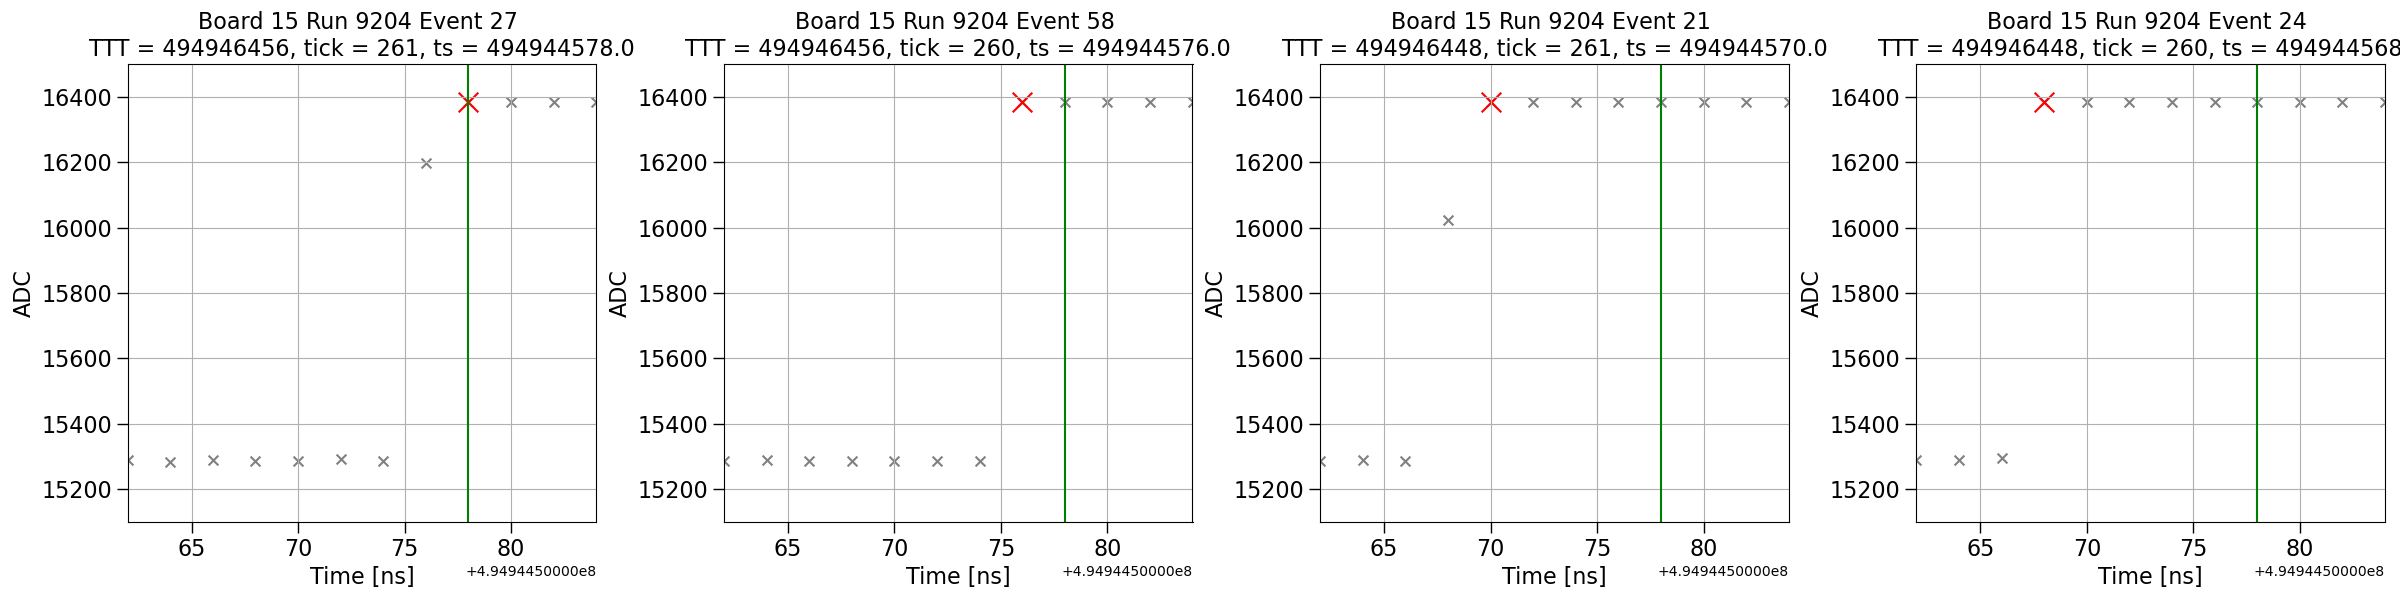
\includegraphics[width=\linewidth]{jitter_before}
\caption{Before Correction}
\label{subfig:jitter_before}
\end{subfigure}

\hfill
\begin{subfigure}[h]{1.00\linewidth}
\centering    
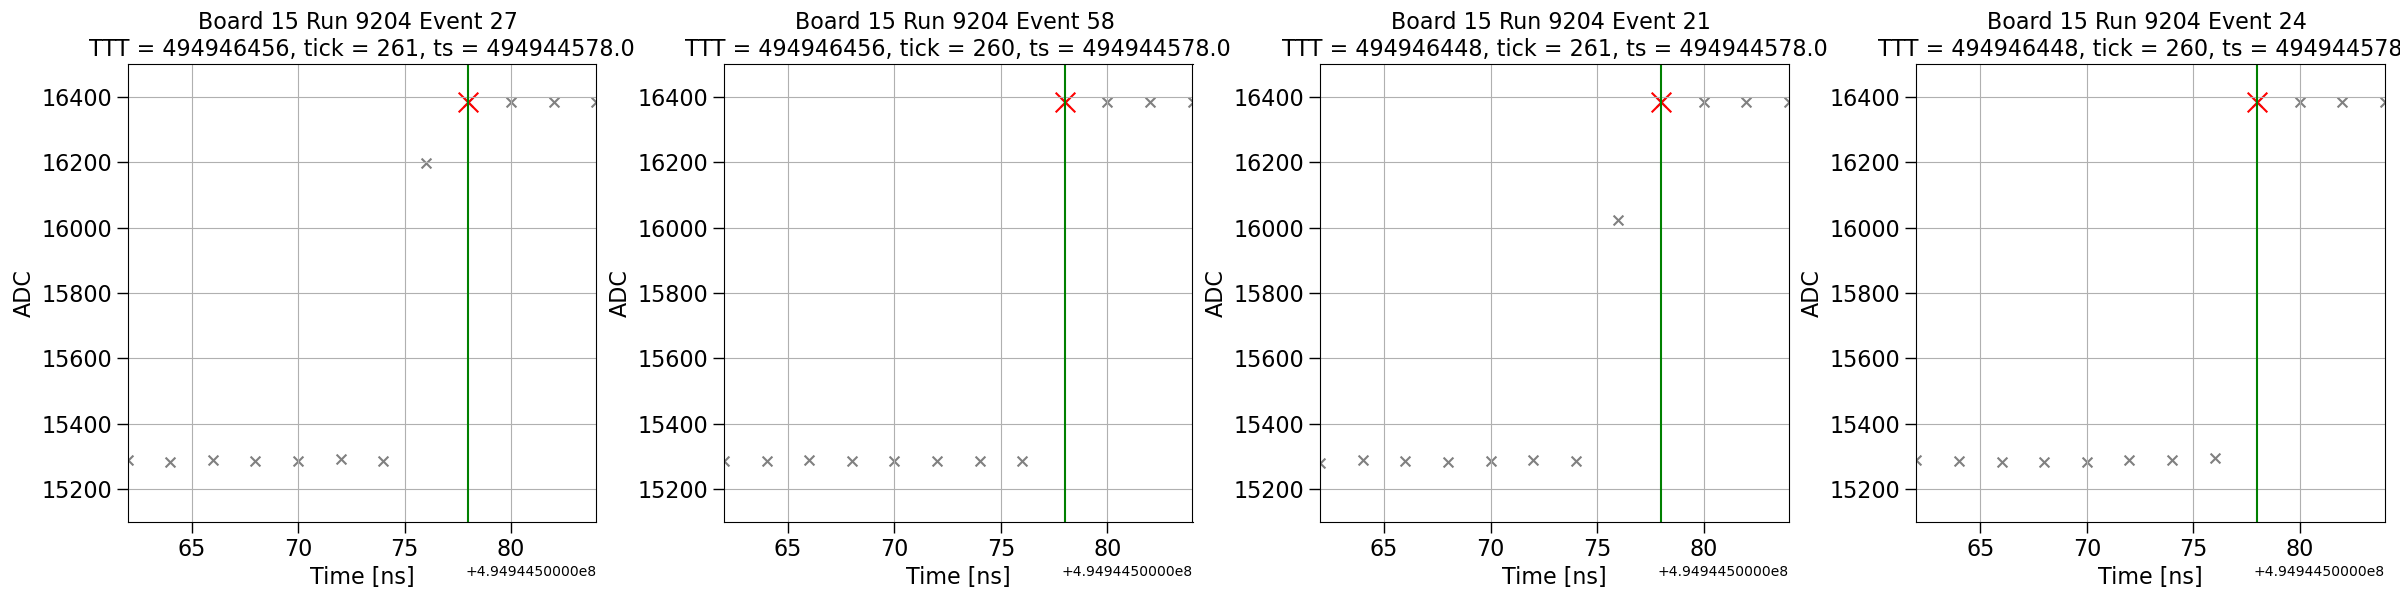
\includegraphics[width=\linewidth]{jitter_after}
\caption{After Correction}
\label{subfig:jitter_after}
\end{subfigure}%

\caption[jitterCorr]{
These plots show the zoomed in of the rising edge position of the trigger waveforms.
The far left plot show a synchronised event where no correction is needed for comparison.
For the rest of the plots from left to right, three cases of jittering are shown and their effects on both the TTT value and tick value of the rising edge.
The first case only contains the jittering of the ADC sampling clock, requiring a correction of 2 ns.
The second case only contains the jittering of the trigger clock, requiring a correction of 8 ns.
The third case contains the jittering from both of the clocks, thus the correction contains a combined smearing of 10 ns.
}
\label{fig:jitterCorr}
\end{figure}

\begin{figure}[htbp!]

\begin{subfigure}[h]{1.00\linewidth}
\centering    
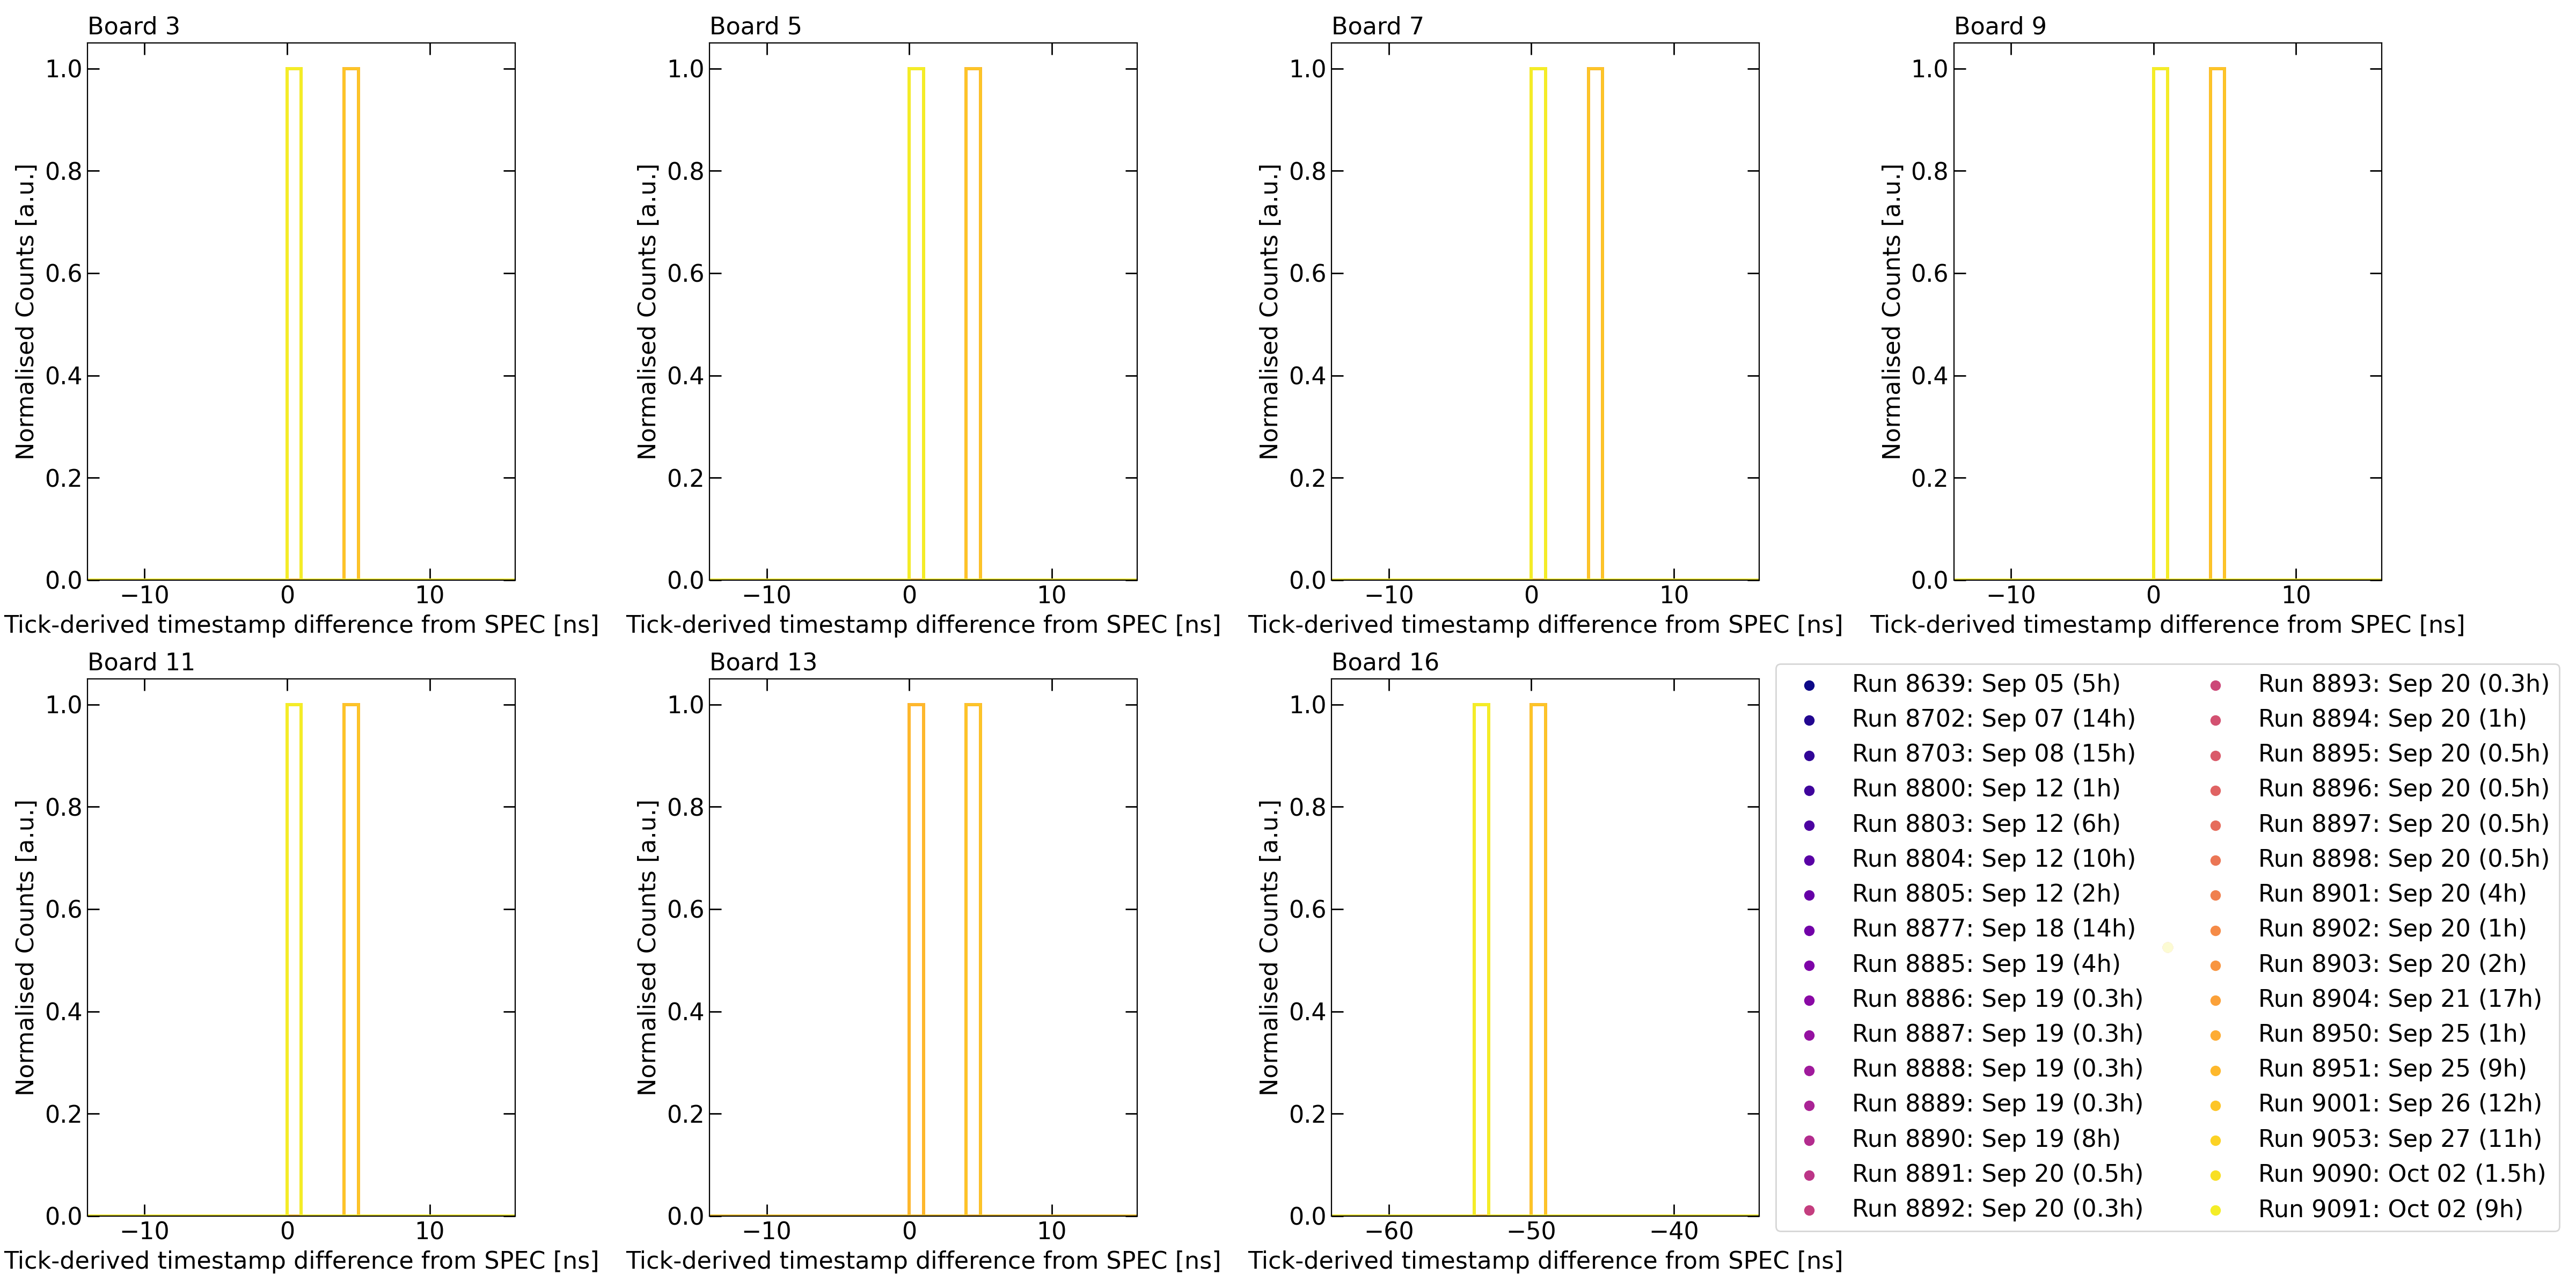
\includegraphics[width=\linewidth]{Tickts_spec_corrEbyE}
\caption{After Correction Event By Event}
\label{subfig:Tickts_spec_corrEbyE}
\end{subfigure}

\hfill
\begin{subfigure}[h]{1.00\linewidth}
\centering    
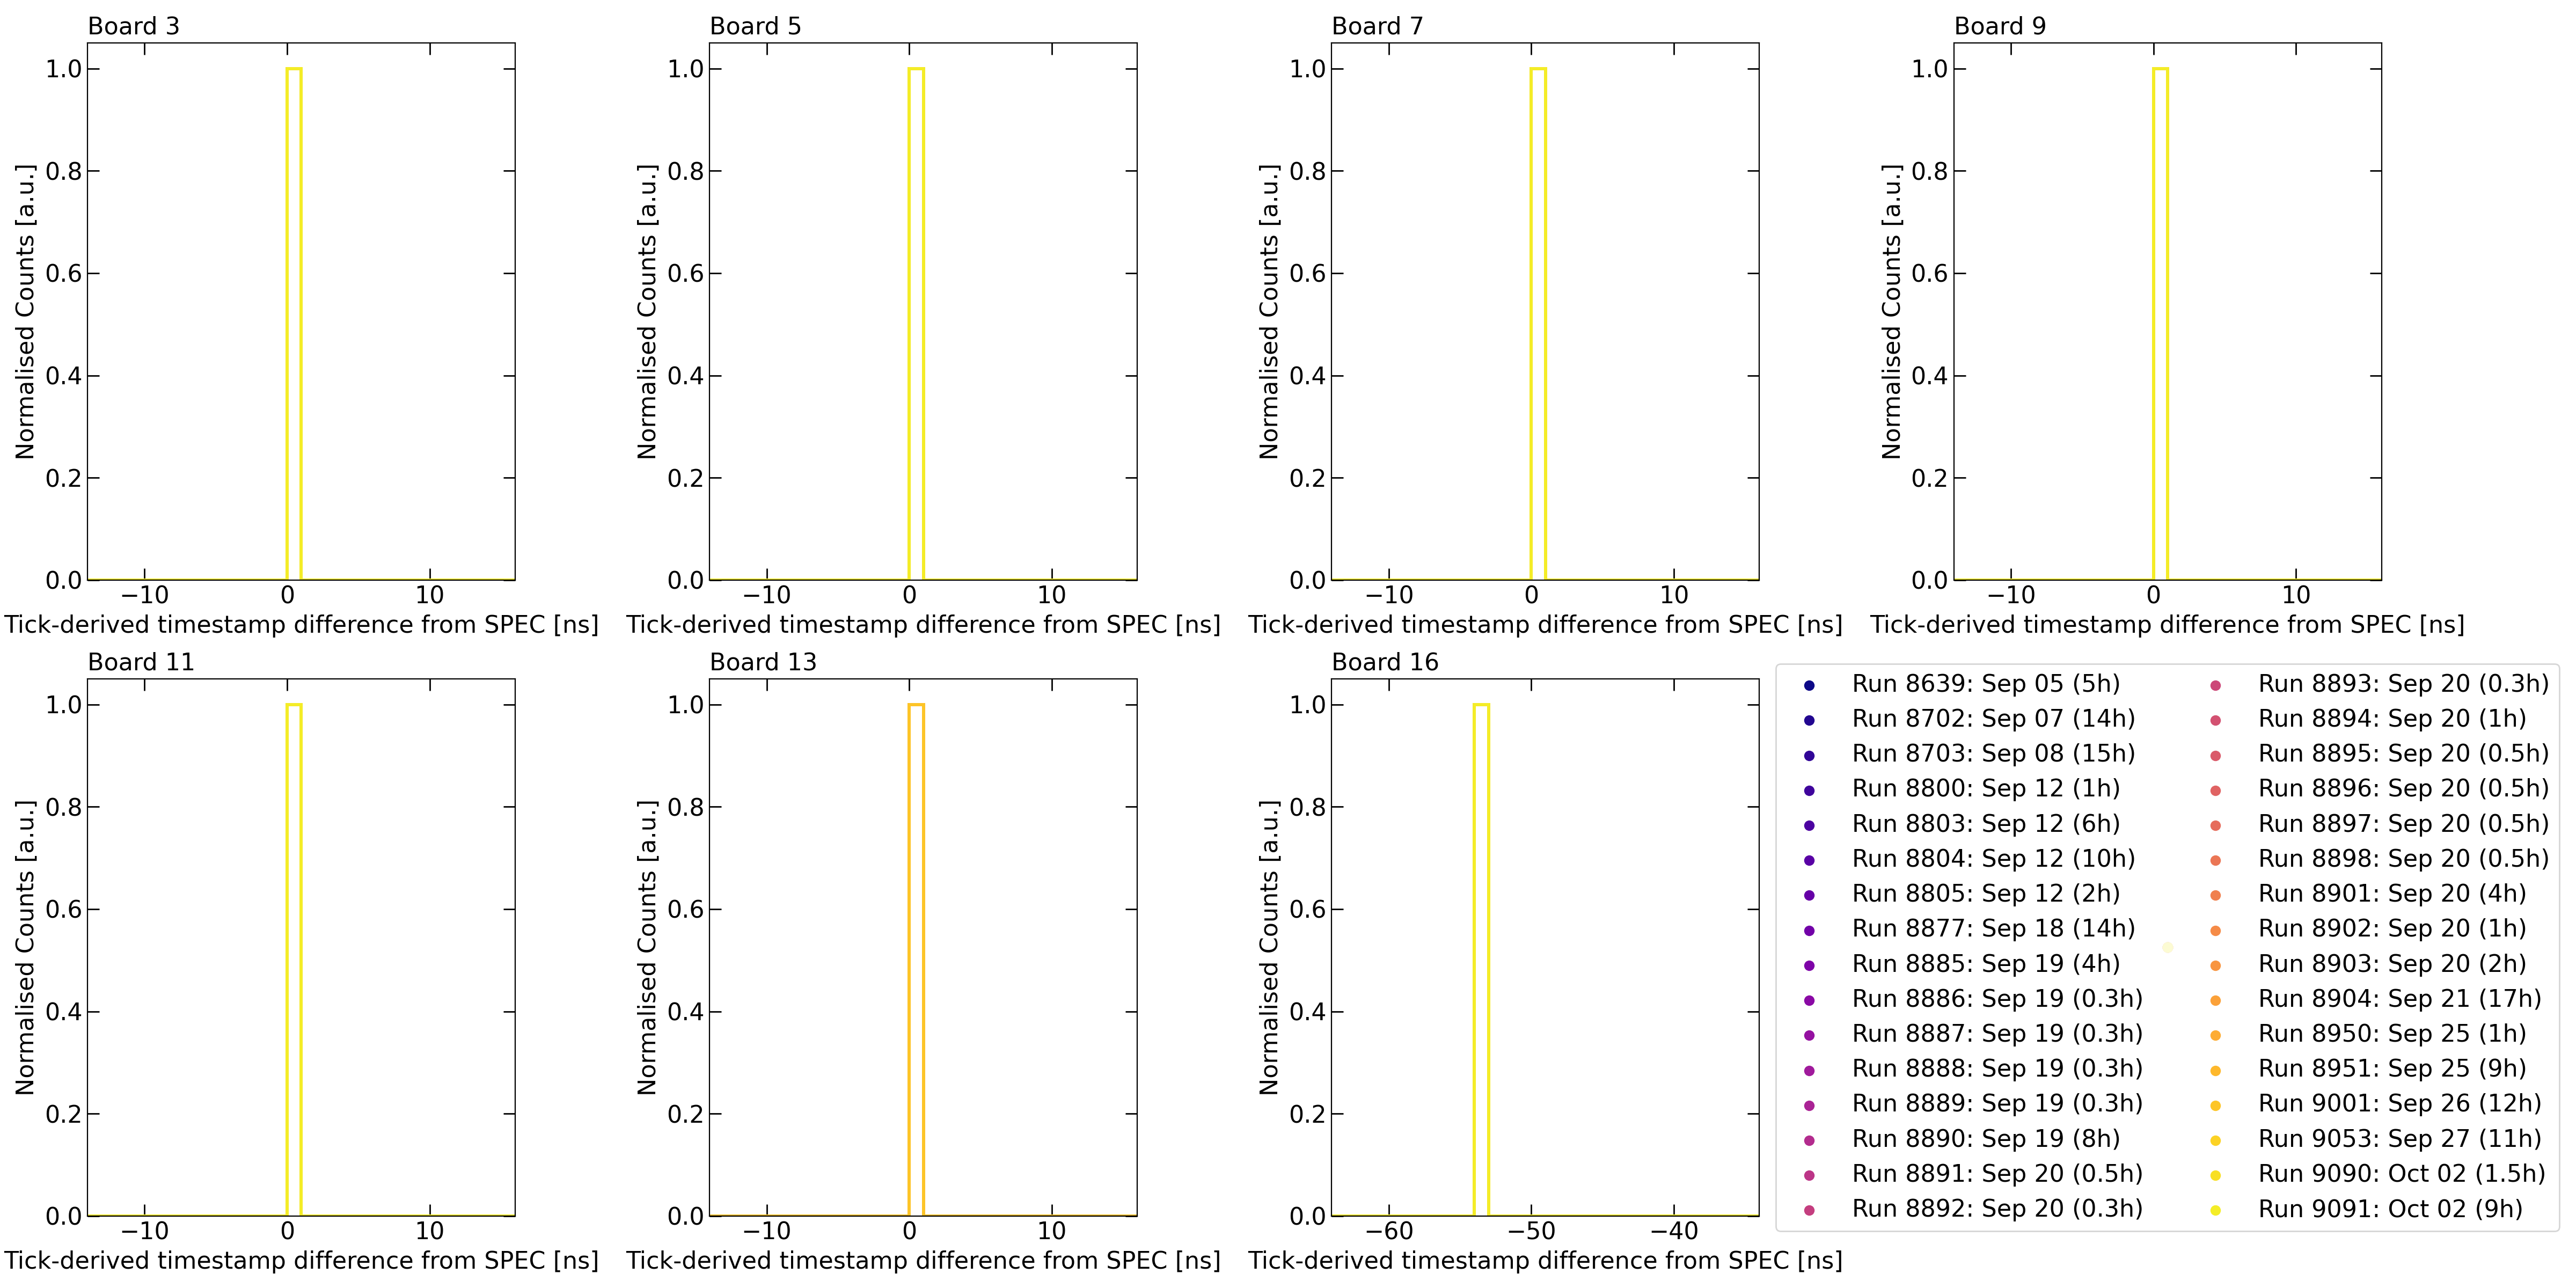
\includegraphics[width=\linewidth]{Tickts_spec_corrRbyR}
\caption{After Correction Run by Run}
\label{subfig:Tickts_spec_corrRbyR}
\end{subfigure}%

\caption[jitterCorrEbyERbyR]{
The jittering correction to the tick-derived timestamp was applied in steps of event by event, followed by run by run.
This results in perfect synchronisation across all digitizers and with respect to the PPS signal.
Board 16 is an exception due to having different firmware. 
This jittering correction workflow still reveals the amount of correction for this board, which is -54 ns. 
An additional correction step can be taken to account for time synchronisation across digitizers with different firmwares. 
}
\label{fig:Tickts_spec_corr}
\end{figure}

%how to correct for jittering:
By digitising the trigger signal synchronously on every digitizer, the recorded waveform of the trigger provides all the necessary information to apply correction.
One can simply derive the correction amount by comparing the tick-derived timestamp of the trigger signal from one event to another, as illustrated in Fig. \ref{subfig:jitter_after}.
Once this correction is applied to all events within the same run, one can also correct for the random clock phase initialisation across multiple runs within the same CAEN digitizer.
This order of correction results in the perfect synchronisation across all events and all runs from different periods of time.
For demonstration, this correction workflow was applied to the distribution of the tick-derived timestamp previously shown in Fig. \ref{subfig:Tickts_spec}.
The correction was applied event by event followed by correction run by run as shown in Fig. \ref{fig:Tickts_spec_corr}, resulting in synchronisation across all the CAEN digitizers and also with respect to the PPS signal.

\begin{figure}[htbp!] 
\centering    
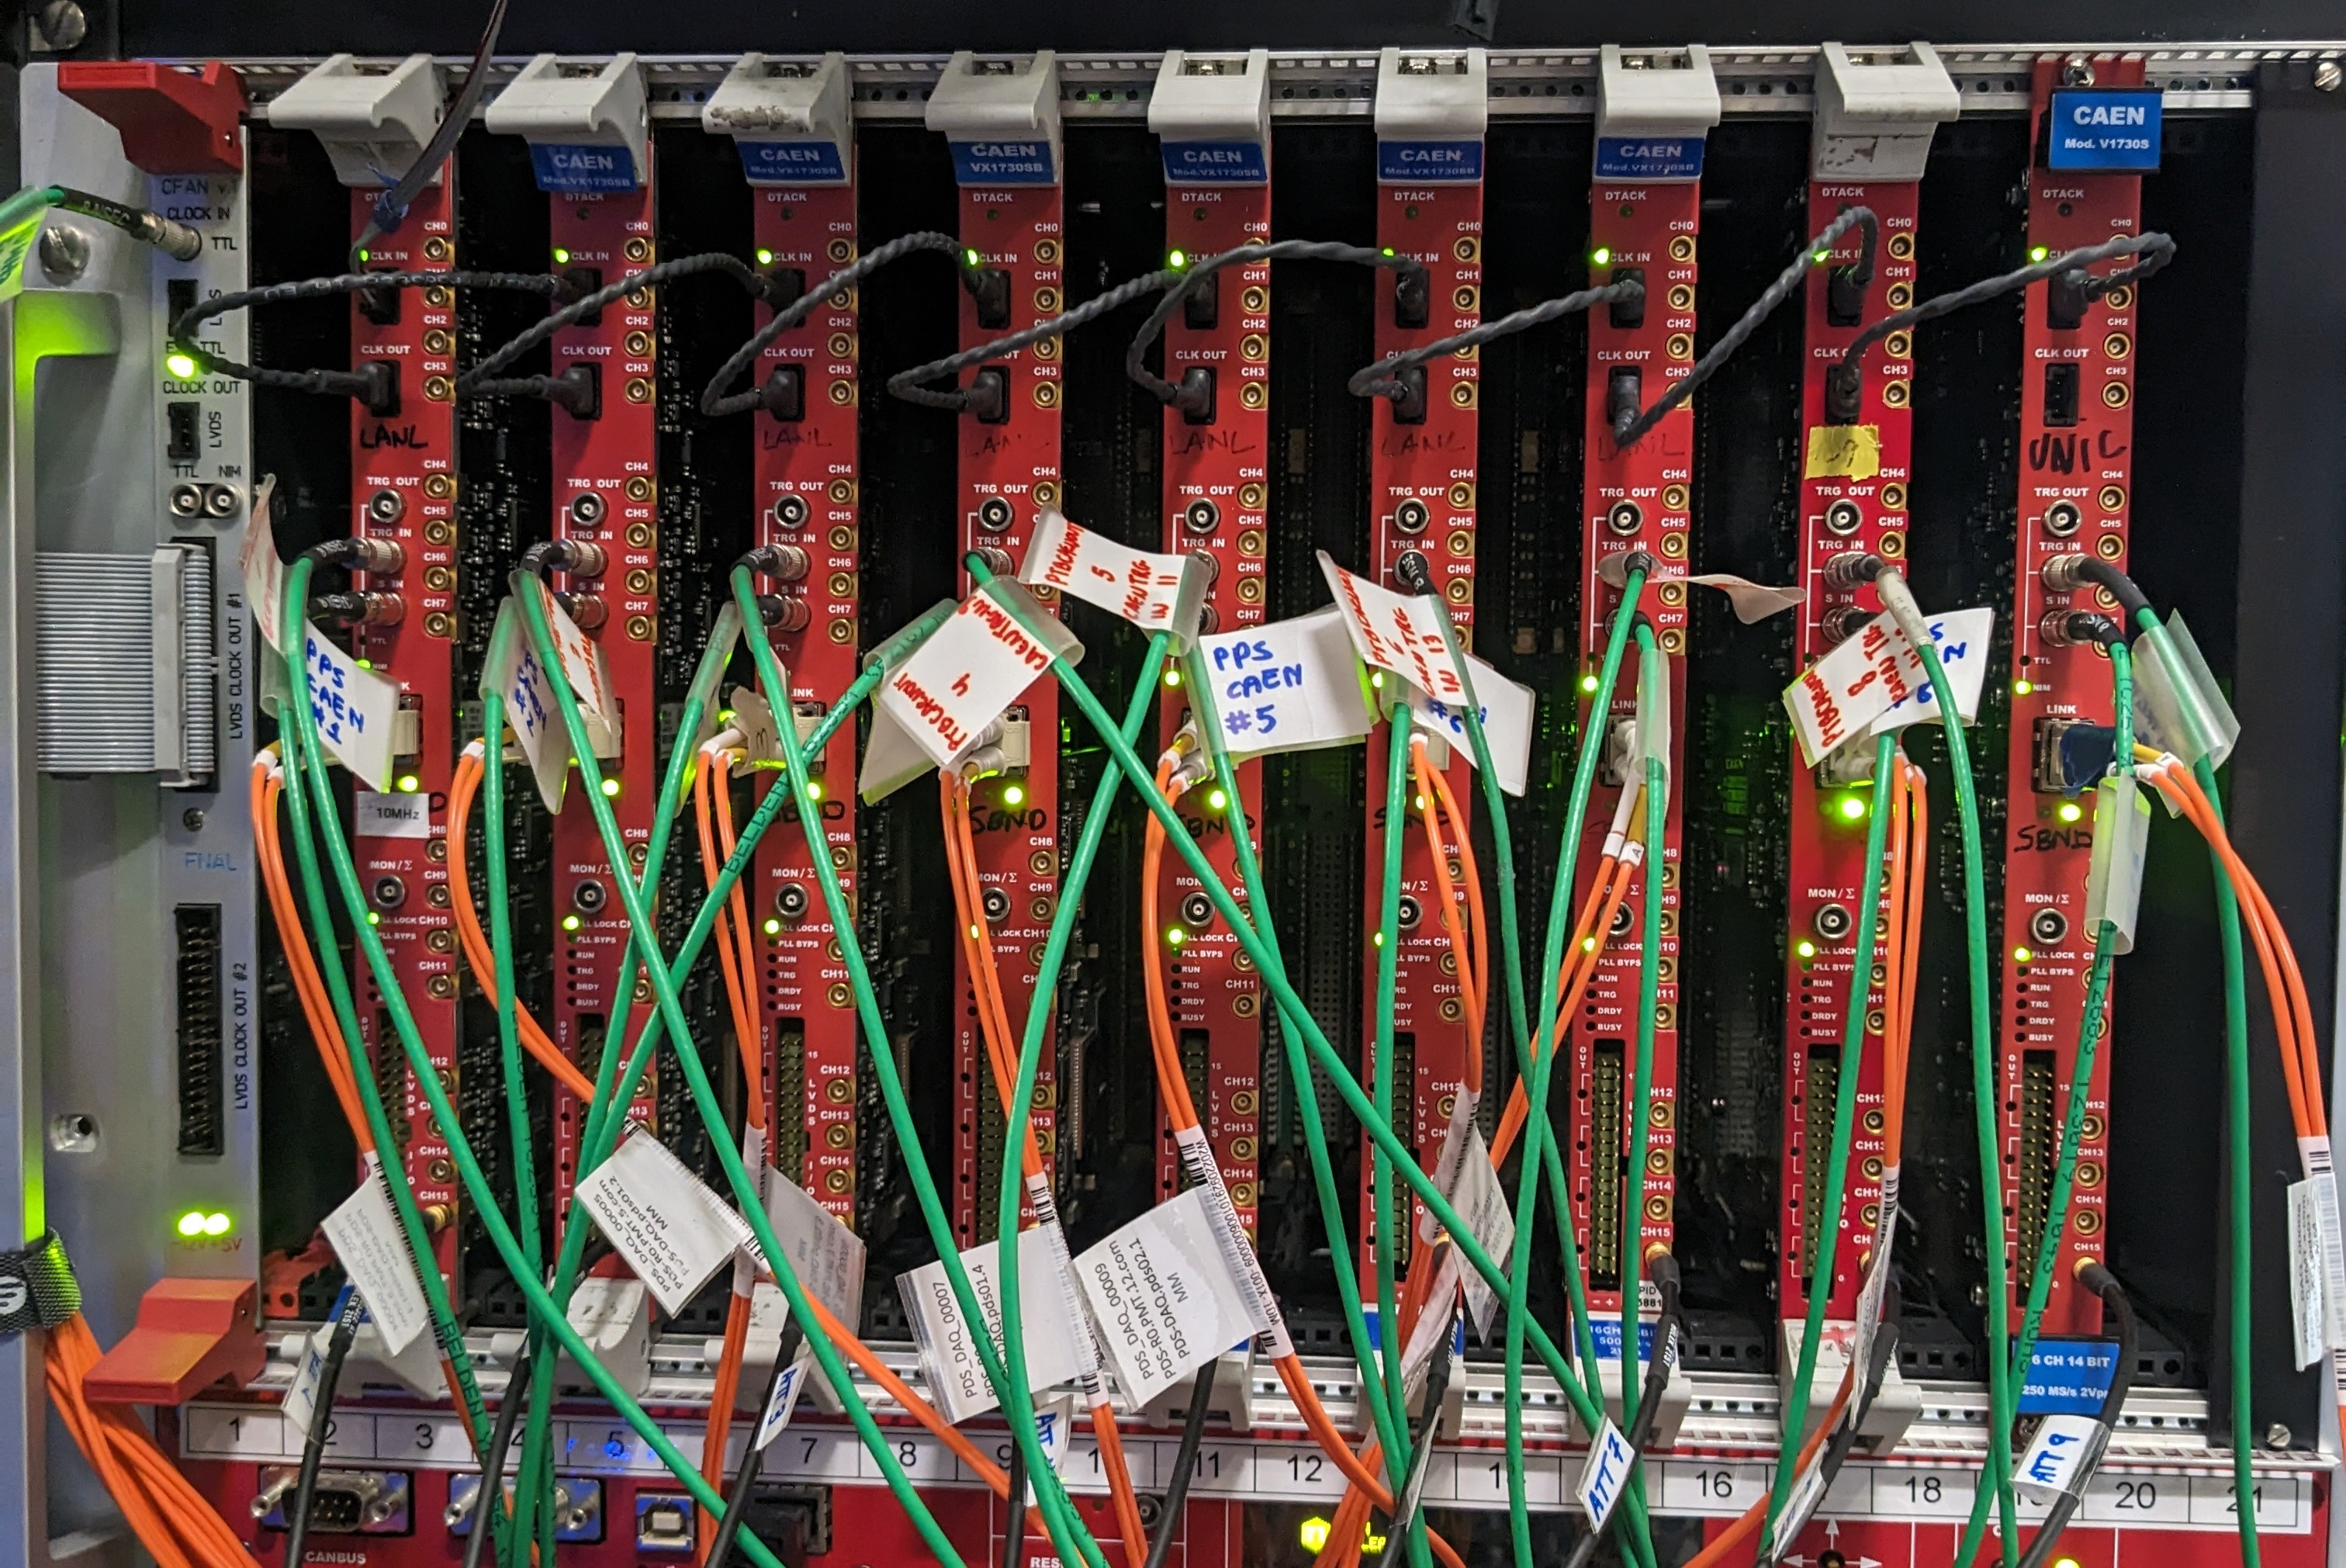
\includegraphics[width=0.6\textwidth]{pds_r0}
\caption[pdsR0]{
Photograph of the final set up for the PDS-R0 rack, which houses 8 CAEN digitizers for digitizing the PMTs, and a new addition 9th CAEN digitizers for digitizing the beam signals.
The daisy chain clock scheme is chosen, and channel 15 of every digitizer is input with the trigger signals to digitize the waveforms.
The waveform will contain necessary information for jittering correction in downstream analysis.
}
\label{fig:pdsR0}
\end{figure}

This study has resulted in a new hardware proposal by the author for physics run at SBND.
The proposal suggested to digitize the trigger signal in all channel 15 of every CAEN digitizer such that this will provide the necessary timing information for downstream jittering correction.
This new cable connection requires an additional CAEN digitizer since the original plan was to digitize beam signals in channel 15.
The new CAEN digitizer will be used solely for recording beam signals such as the BES and RWM signal.
The installation of the new hardware setup was carried out by the author during her time at Fermilab and this is photographed in Fig. \ref{fig:pdsR0}.


%********************************** %Third Section  **************************************
\section{Concluding Remarks}
\label{sec5Remarks}

The DAQ system of the SBND experiment has been outlined, detailing the overall process involved in constructing a physics event from various hardware subsystems. 
The event building process relies heavily on precise timing synchronization across these subsystems, achieved through the implementation of the WR timing system.
Each readout electronic device is synced with a PPS signal derived from the WR devices, ensuring that the timestamps of recorded events from each hardware component align with the frame of reference relative to the PPS signal.
The evaluation of the timing resolution of the readout electronics of the CRTs, which are the FEB modules, was presented. 
The timing resolution of the FEB modules was observed to be approximately 2 ns for both the T0 and T1 internal clocks.
Exploration into an alternative timing reconstruction method using timestamps from the T0 clock, combined with the SPEC-TDC, was undertaken. 
This method reconstructed the beam spill structure and substructure, demonstrating good agreement when compared to using timestamps from the T1 clock.
Additionally, an evaluation was conducted on the readout electronics for the PMTs, namely the CAEN digitizers, focusing on timing synchronization and resolution. 
The work resulted in the daisy chain clock scheme was chosen to synchronise all the digitizers within the same crate.
Furthermore, a method for jittering correction was devised by simultaneously digitising trigger waveforms in each digitizer. 
This correction method allows for absolute timing synchronization across all the CAEN digitizers as well as with the PPS signal up to resolution of 1 ns.

